\chapter{The First 16 Milliseconds} 
\label{sec:first16}
\lstset{style=6502Style}
OK, where were we? At the end of \hyperref[sec:archaeo]{\textcolor{blue}{A Little Archaeology}}
we were just about to get started and begin the race to get something up on the screen.
We had set up an interrupt to make us jump to \icode{MainControlLoop} at address \icode{\$4000}.

Our first act in \icode{MainControlLoop} is to make sure that the next interrupt didn't
have us jumping to the start of \icode{MainControlLoop} all over again. So we overwrite the interrupt handler with a new address,
\icode{MainControlLoopInterruptHandler}. You will be reassured to learn that, having the changed the interrupt 
handler three times in several milliseconds, we are ready to settle down and stick with \icode{MainControlLoop\-Interrupt\-Handler} as our
interrupt handler of choice for the time being:

\begin{lstlisting}[caption=The code at \icode{\$4000}. ,escapechar=\%]
MainControlLoop%\index{MainControlLoop}%
        LDA #$00
        SEI
p4003   LDA #<MainControlLoopInterruptHandler%\index{MainControlLoopInterruptHandler}%
        STA $318    ;NMI
        LDA #>MainControlLoopInterruptHandler%\index{MainControlLoopInterruptHandler}%
        STA $319    ;NMI
\end{lstlisting}

Our next act is to call a routine\index{routine} to set up the main title screen\index{screen}:

\begin{lstlisting}[caption=In \icode{MainControlLoop\index{MainControlLoop}},escapechar=\%]
        ; Display the title screen%\index{screen}%. We'll stay in here until the
        ; player presses fire or we time out and go into attract mode.
        JSR EnterMainTitleScreen%\index{EnterMainTitleScreen}%
\end{lstlisting}

\icode{EnterMainTitleScreen} does a bit of shuffling of data before it brings
us to a routine\index{routine} that does something important. This routine is called
\icode{InitializeSpritesAndInterruptsForTitleScreen\index{InitializeSpritesAndInterruptsForTitleScreen}}
and it does some vital setup for the next 16 milliseconds that determines how we go
about getting everything on the screen\index{screen} that we need to get:
\begin{lstlisting}[caption=In \icode{InitializeSpritesAndInterruptsForTitleScreen\index{InitializeSpritesAndInterruptsForTitleScreen}},escapechar=\%]
        ; Set up the our interrupt%\index{interrupt}% handler for the title
        ; screen%\index{screen}%. This will do all the animation%\index{animation}% and title
        ; music work.
        LDA #<TitleScreenInterruptHandler%\index{TitleScreenInterruptHandler}%
        STA $0314    ;IRQ
        LDA #>TitleScreenInterruptHandler%\index{TitleScreenInterruptHandler}%
        STA $0315    ;IRQ

        ; Acknowledge the interrupt%\index{interrupt}%, so the CPU knows that
        ; we have handled it.
        LDA #$01
        STA $D019    ;VIC Interrupt%\index{Interrupt}% Request Register%\index{Register}% (IRR)
        STA $D01A    ;VIC Interrupt%\index{Interrupt}% Mask Register%\index{Register}% (IMR)

        ; Set up the raster interrupt%\index{interrupt}% to happen when the
        ; raster reaches the position we specify in D012.
        LDA $D011    ;VIC Control Register%\index{Register}% 1
        AND #$7F
        STA $D011    ;VIC Control Register%\index{Register}% 1

        ; Set the position for triggering our interrupt%\index{interrupt}%.
        LDA #$10
        STA $D012    ;Raster Position
\end{lstlisting}

You'll notice we've changed yet another interrupt\index{interrupt} handler, this time to a routine\index{routine} called
\icode{TitleScreenInterruptHandler\index{TitleScreenInterruptHandler}}. I didn't lie to you earlier though. This is not
the same interrupt we settled on above. It is a new and important one that affects how get things on to the screen.
The particular type of interrupt\index{interrupt} it is concerned with is something
called a 'Raster Interrupt\index{Interrupt}'. A 'raster' can be thought of as a beam of light that scans
across the screen\index{screen} from top to bottom and left to right, painting each pixel on the screen\index{screen}
one at a time. It travels so quickly down and across the screen\index{screen} painting pixels that it
can do so up to 60 times a second.

As it makes this journey our 'Raster Interrupt\index{Interrupt}' gives
us the opportunity to tell it to stop once it reaches a certain position on the screen\index{screen}
and allows us to run some code before it resumes again. We can do this as many times as
we want along the journey, but each time we interrupt\index{interrupt} it we have to be quick. If our code
takes too long the display will flicker and the content of the screen\index{screen} become inconsistent.

At the very end of the little listing above we set our first interrupt\index{interrupt} to line 16 (\icode{\$10}) on the screen\index{screen}:
\clearpage

\begin{lstlisting}[caption=In \icode{InitializeSpritesAndInterruptsForTitleScreen\index{InitializeSpritesAndInterruptsForTitleScreen}},escapechar=\%]
        ; Set the position for triggering our interrupt%\index{interrupt}%.
        LDA #$10
        STA $D012    ;Raster Position
\end{lstlisting}

This facility is the key that will allow us to do all sorts of magic in the 16 milliseconds
it takes to traverse the screen\index{screen}. Every time we get the opportunity to run some code thanks
to this interrupt\index{interrupt} we'll change the location of the screen\index{screen} it should stop at the next time
so that we get to stop dozens of times in each single 16 millisecond traversal.

Before we look at how we fit it all in, let's first appreciate just how much we plan to
do each time the screen\index{screen} is painted\index{painted}.

\section{Sprites\index{Sprites}}
The C64 makes 8 sprites\index{sprites} available to us. A sprite is a special purpose graphical object that
can be up to 24 pixels wide by 20 pixels high. We can place them wherever we want on the
screen\index{screen}. They are the core of graphics\index{graphics} programming and Iridis Alpha has dozens of them. 

\begin{figure}[H]
  {
    \setlength{\tabcolsep}{1.0pt}
    \setlength\cmidrulewidth{\heavyrulewidth} % Make cmidrule = 
    \begin{adjustbox}{width=4cm,center}
	\begin{subfigure}{0.3\textwidth}
    \def\MULTICOLORONE{red}
    \def\MULTICOLORTWO{white}
    \def\SPRITECOLOR{blue}
		\input{sprites/GILBY_AIRBORNE_LEFT}
	\end{subfigure}
    \end{adjustbox}
  }\caption{An example of a sprite in Iridis Alpha.}
\end{figure}


But if the C64 only has 8 sprites\index{sprites}, are we limited to displaying
just 8 sprites\index{sprites} at once on the screen\index{screen}?

The simple
answer is that thanks to \textit{Raster Interrupts} we are not: when we run
some code after receiving an interrupt\index{interrupt} we can place new
sprites\index{sprites} wherever we like in any position that the raster hasn't
reached yet. This means our only effective limitation is the number of
sprites\index{sprites} we can place on a single line, which is eight.  If you look carefully at the title screen\index{screen} of Iridis Alpha you'll notice that it is actually
split in two.

\begin{figure}[H]
  {
    \begin{adjustbox}{width=10cm,center}
      \frame{\surface{titlescreen/ia-title3.png}}
    \end{adjustbox}
  }
\caption{The title screen with big letters up top and jumping gilbies down below.}
\end{figure}

The top half has the title in large letters and the bottom half has a rainbow\index{rainbow}
of jumping\index{jumping} gilbies\index{gilbies}. Each half uses seven sprites\index{sprites} (numbered 0 to 6) to display these assets.


\begin{figure}[H]
  {
    \setlength{\tabcolsep}{1.0pt}
    \setlength\cmidrulewidth{\heavyrulewidth} % Make cmidrule = 
    \begin{adjustbox}{width=14cm,center}
      \begin{tabular}{ccccccc}
        \toprule
        Sprite0 & Sprite1 & Sprite2 & Sprite3 & Sprite4 & Sprite5 & Sprite6 \\
        \midrule
\makecell[l]{
	\begin{subfigure}{0.3\textwidth}
    \def\MULTICOLORONE{gray}
    \def\MULTICOLORTWO{black}
    \def\SPRITECOLOR{red}
		\input{sprites/BIG_I}
	\end{subfigure}
} &
\makecell[l]{
	\begin{subfigure}{0.3\textwidth}
    \def\MULTICOLORONE{gray}
    \def\MULTICOLORTWO{black}
    \def\SPRITECOLOR{orange}
		\input{sprites/BIG_R}
	\end{subfigure}
} &
\makecell[l]{
	\begin{subfigure}{0.3\textwidth}
    \def\MULTICOLORONE{gray}
    \def\MULTICOLORTWO{black}
    \def\SPRITECOLOR{yellow}
		\input{sprites/BIG_I}
	\end{subfigure}
} &
\makecell[l]{
	\begin{subfigure}{0.3\textwidth}
    \def\MULTICOLORONE{gray}
    \def\MULTICOLORTWO{black}
    \def\SPRITECOLOR{green}
		\input{sprites/BIG_D}
	\end{subfigure}
} &
\makecell[l]{
	\begin{subfigure}{0.3\textwidth}
    \def\MULTICOLORONE{gray}
    \def\MULTICOLORTWO{black}
    \def\SPRITECOLOR{cyan}
		\input{sprites/BIG_I}
	\end{subfigure}
} &
\makecell[l]{
	\begin{subfigure}{0.3\textwidth}
    \def\MULTICOLORONE{gray}
    \def\MULTICOLORTWO{black}
    \def\SPRITECOLOR{pink}
		\input{sprites/IG_S}
	\end{subfigure}
} &
\makecell[l]{
	\begin{subfigure}{0.3\textwidth}
    \def\MULTICOLORONE{gray}
    \def\MULTICOLORTWO{gray}
    \def\SPRITECOLOR{gray}
		\input{sprites/ALPHA}
	\end{subfigure}
} \\ 
        \midrule
\makecell[l]{
	\begin{subfigure}{0.3\textwidth}
    \def\MULTICOLORONE{gray}
    \def\MULTICOLORTWO{white}
    \def\SPRITECOLOR{red}
		\input{sprites/LAND_GILBY4}
	\end{subfigure}
} & 
\makecell[l]{
	\begin{subfigure}{0.3\textwidth}
    \def\MULTICOLORONE{gray}
    \def\MULTICOLORTWO{white}
    \def\SPRITECOLOR{orange}
		\input{sprites/LAND_GILBY4}
	\end{subfigure}
} & 
\makecell[l]{
	\begin{subfigure}{0.3\textwidth}
    \def\MULTICOLORONE{gray}
    \def\MULTICOLORTWO{white}
    \def\SPRITECOLOR{yellow}
		\input{sprites/LAND_GILBY4}
	\end{subfigure}
} & 
\makecell[l]{
	\begin{subfigure}{0.3\textwidth}
    \def\MULTICOLORONE{gray}
    \def\MULTICOLORTWO{white}
    \def\SPRITECOLOR{green}
		\input{sprites/LAND_GILBY4}
	\end{subfigure}
} & 
\makecell[l]{
	\begin{subfigure}{0.3\textwidth}
    \def\MULTICOLORONE{gray}
    \def\MULTICOLORTWO{white}
    \def\SPRITECOLOR{cyan}
		\input{sprites/LAND_GILBY4}
	\end{subfigure}
} & 
\makecell[l]{
	\begin{subfigure}{0.3\textwidth}
    \def\MULTICOLORONE{gray}
    \def\MULTICOLORTWO{white}
    \def\SPRITECOLOR{pink}
		\input{sprites/LAND_GILBY4}
	\end{subfigure}
} & 
\makecell[l]{
	\begin{subfigure}{0.3\textwidth}
    \def\MULTICOLORONE{gray}
    \def\MULTICOLORTWO{white}
    \def\SPRITECOLOR{purple}
		\input{sprites/LAND_GILBY4}
	\end{subfigure}
} \\ 
        \addlinespace
        \bottomrule
      \end{tabular}
    \end{adjustbox}
  }\caption{The sprites\index{sprites} used by the top half of the screen\index{screen} and the bottom half of the screen\index{screen}.}
\end{figure}

The eighth sprite (Sprite 7) is used on both halves of the screen\index{screen} to display the starfield\index{starfield}. This
sprite pushes right up against the line limitation. It's painted\index{painted} at intervals throughout the screen\index{screen}
but we're careful to avoid it ever being painted\index{painted} twice on the same line. We'll see how this is
achieved very soon.


\begin{figure}[H]
  {
    \setlength{\tabcolsep}{1.0pt}
    \setlength\cmidrulewidth{\heavyrulewidth} % Make cmidrule = 
    \begin{adjustbox}{width=4cm,center}
	\begin{subfigure}{0.3\textwidth}
    \def\MULTICOLORONE{gray}
    \def\MULTICOLORTWO{gray}
    \def\SPRITECOLOR{gray}
		\input{sprites/STARFIELD_SPRITE}
	\end{subfigure}
    \end{adjustbox}
  }\caption{The sprite used for painting the starfield\index{starfield}. Only a part of the sprite is ever painted\index{painted}!}
\end{figure}

\section{Waiting for the Beam}
With our 'Raster Interrupt\index{Interrupt}' handler set up as \icode{TitleScreenInterruptHandler\index{TitleScreenInterruptHandler}} we're ready to 
react when the raster reaches line 16 on the screen\index{screen}. Since the screen\index{screen} is made up of 512 lines in
total this will be along soon.

Before it comes to getus we just have time to prepare the relatively light amount of text we want displayed
on the screen\index{screen} in memory. We only need to do this once. Throughout the code we refer to this
area we write to as \icode{SCREEN\_RAM}. It's an address range between \icode{\$0400} and \icode{\$07E8} This is a very
simple bitmap representation of the entire screen\index{screen} that is 40 characters wide and 25 characters high,
giving a total of 1000 bytes (\icode{\$3E8} bytes in hex). If we wanted to think of it as pixels it is 320 pixels wide (40 * 8)
and 200 pixels high (25 * 8). The important thing to remember about this \icode{SCREEN\_RAM} is that it is solely
for storing what we call character\index{character} data. You can think of character\index{character} data as 'text'. This text gets painted\index{painted}
first and then sprites\index{sprites} get painted\index{painted} on top of it.

In \icode{EnterTitleScreenLoop\index{EnterTitleScreenLoop}} we call two routines that will prepare the character\index{character} data for the raster to paint. 

The first, \icode{DrawStripesBehindTitle\index{DrawStripesBehindTitle}} writes the rainbow\index{rainbow} stripes to five lines in the top half of the screen\index{screen}. 
The second, \icode{DrawTitleScreenText\index{DrawTitleScreenText}} writes some text to the bottom half of the screen\index{screen}. Before we look at these
in detail we need to understand how this thing \icode{SCREEN\_RAM} works and how we store characters for display in it.

Our starting point for displaying text on screen\index{screen} is to define what our characters look like. We define the appearance
of a character\index{character} using 8 bytes. This is what the definition of the stripe character\index{character} looks like: 

\clearpage
\begin{lstlisting}[caption= The 'stripe' character\index{character}.,escapechar=\%]
characterSetData%\index{characterSetData}%
.BYTE $FF,          ; 11111111   ********
.BYTE $00,          ; 00000000           
.BYTE $FF,          ; 11111111   ********
.BYTE $00,          ; 00000000           
.BYTE $00,          ; 00000000           
.BYTE $FF,          ; 11111111   ********
.BYTE $00           ; 00000000           
.BYTE $FF,          ; 11111111   ********
\end{lstlisting}

As you can see each byte translates to a row of 0s and 1s. Each 1 defines a dot and each 0 a blank space. We end up
with a character\index{character} that is 8 pixels wide and 8 pixels high:


    \begin{figure}[H]
      {
        \setlength{\tabcolsep}{3.0pt}
        \setlength\cmidrulewidth{\lightrulewidth} % Make cmidrule = 
        \begin{adjustbox}{width=6cm,center}
          \begin{tikzpicture}
    
\def\CHARCOLOR{lightgray}
	\draw[step=1.0,gray,thin] (0,0) grid (8,8);
	\fill[\CHARCOLOR] (0,7) rectangle ++ (1,1);
	\fill[\CHARCOLOR] (1,7) rectangle ++ (1,1);
	\fill[\CHARCOLOR] (2,7) rectangle ++ (1,1);
	\fill[\CHARCOLOR] (3,7) rectangle ++ (1,1);
	\fill[\CHARCOLOR] (4,7) rectangle ++ (1,1);
	\fill[\CHARCOLOR] (5,7) rectangle ++ (1,1);
	\fill[\CHARCOLOR] (6,7) rectangle ++ (1,1);
	\fill[\CHARCOLOR] (7,7) rectangle ++ (1,1);
	\fill[\CHARCOLOR] (0,5) rectangle ++ (1,1);
	\fill[\CHARCOLOR] (1,5) rectangle ++ (1,1);
	\fill[\CHARCOLOR] (2,5) rectangle ++ (1,1);
	\fill[\CHARCOLOR] (3,5) rectangle ++ (1,1);
	\fill[\CHARCOLOR] (4,5) rectangle ++ (1,1);
	\fill[\CHARCOLOR] (5,5) rectangle ++ (1,1);
	\fill[\CHARCOLOR] (6,5) rectangle ++ (1,1);
	\fill[\CHARCOLOR] (7,5) rectangle ++ (1,1);
	\fill[\CHARCOLOR] (0,2) rectangle ++ (1,1);
	\fill[\CHARCOLOR] (1,2) rectangle ++ (1,1);
	\fill[\CHARCOLOR] (2,2) rectangle ++ (1,1);
	\fill[\CHARCOLOR] (3,2) rectangle ++ (1,1);
	\fill[\CHARCOLOR] (4,2) rectangle ++ (1,1);
	\fill[\CHARCOLOR] (5,2) rectangle ++ (1,1);
	\fill[\CHARCOLOR] (6,2) rectangle ++ (1,1);
	\fill[\CHARCOLOR] (7,2) rectangle ++ (1,1);
	\fill[\CHARCOLOR] (0,0) rectangle ++ (1,1);
	\fill[\CHARCOLOR] (1,0) rectangle ++ (1,1);
	\fill[\CHARCOLOR] (2,0) rectangle ++ (1,1);
	\fill[\CHARCOLOR] (3,0) rectangle ++ (1,1);
	\fill[\CHARCOLOR] (4,0) rectangle ++ (1,1);
	\fill[\CHARCOLOR] (5,0) rectangle ++ (1,1);
	\fill[\CHARCOLOR] (6,0) rectangle ++ (1,1);
	\fill[\CHARCOLOR] (7,0) rectangle ++ (1,1);
        \node[matrix of math nodes,anchor=south west,inner sep=0pt,
        nodes={draw,minimum size=1cm,anchor=center},
        column sep=-\pgflinewidth,row sep=-\pgflinewidth]
        {\icode{1} & \icode{1}  & \icode{1} & \icode{1} & \icode{1} & \icode{1} & \icode{1} & \icode{1}\\
        \icode{0} & \icode{0}  & \icode{0} & \icode{0} & \icode{0} & \icode{0} & \icode{0} & \icode{0}\\
        \icode{1} & \icode{1}  & \icode{1} & \icode{1} & \icode{1} & \icode{1} & \icode{1} & \icode{1}\\
        \icode{0} & \icode{0}  & \icode{0} & \icode{0} & \icode{0} & \icode{0} & \icode{0} & \icode{0}\\
        \icode{0} & \icode{0}  & \icode{0} & \icode{0} & \icode{0} & \icode{0} & \icode{0} & \icode{0}\\
        \icode{1} & \icode{1}  & \icode{1} & \icode{1} & \icode{1} & \icode{1} & \icode{1} & \icode{1}\\
        \icode{0} & \icode{0}  & \icode{0} & \icode{0} & \icode{0} & \icode{0} & \icode{0} & \icode{0}\\
        \icode{1} & \icode{1}  & \icode{1} & \icode{1} & \icode{1} & \icode{1} & \icode{1} & \icode{1}\\};

          \end{tikzpicture}
        \end{adjustbox}
      }\caption*{The stripe chracter}
    \end{figure}
    


We create this definition for every character\index{character} we want to display and store it at the address starting at \icode{\$2000}
in RAM, which we will give the label \icode{characterSetData}. The order in which we store them determines the reference we use for them later. So for example the stripe
character\index{character} is referred to as \icode{\$00}, the 'A' character\index{character} we've defined as \icode{\$01} and so on:

\subfile{titlescreen/charset_tilesheet}

With our character\index{character} set defined in the \icode{characterSetData} at address \icode{\$2000} we can now write some text to
the \icode{SCREEN\_RAM} at address \icode{\$0400}. For example, when we write a \icode{\$01} to a position in \icode{SCREEN\_RAM}
it will write an 'A' from our character set to that position. Note that when we write a byte to \icode{SCREEN\_RAM}
we're not yet writing it to the actual screen\index{screen}. This is just a
place in memory that the raster (our beam of light) will refer to later when it
is actually writing dots to the screen\index{screen}. So for example, when we write a stripe (\icode{\$00}) or 'A' (\icode{\$01})
character index to a particular position in this \icode{SCREEN\_RAM}
memory it will know to write it to the corresponding position on the
screen\index{screen}. 

\subsection{Drawing the Stripes}
So let's use our stripe character at position \icode{\$00} in our \icode{characterSetData} to  write some stripes to RAM!

\begin{lstlisting}[caption=Drawing stripes using a loop!,escapechar=\%]
DrawStripesBehindTitle%\index{DrawStripesBehindTitle}%
        LDX #40
        LDA #$00
        STA shouldUpdateTitleScreenColors%\index{shouldUpdateTitleScreenColors}%
DrawStripesLoop%\index{DrawStripesLoop}%   
        LDA #RED
        STA COLOR_RAM%\index{COLOR\_RAM}% + LINE2_COL39%\index{LINE2\_COL39}%,X
        LDA #ORANGE
        STA COLOR_RAM%\index{COLOR\_RAM}% + LINE3_COL39%\index{LINE3\_COL39}%,X
        LDA #YELLOW
        STA COLOR_RAM%\index{COLOR\_RAM}% + LINE4_COL39%\index{LINE4\_COL39}%,X
        LDA #GREEN
        STA COLOR_RAM%\index{COLOR\_RAM}% + LINE5_COL39%\index{LINE5\_COL39}%,X
        LDA #LTBLUE
        STA COLOR_RAM%\index{COLOR\_RAM}% + LINE6_COL39%\index{LINE6\_COL39}%,X
        LDA #PURPLE
        STA COLOR_RAM%\index{COLOR\_RAM}% + LINE7_COL39%\index{LINE7\_COL39}%,X
        LDA #BLUE
        STA COLOR_RAM%\index{COLOR\_RAM}% + LINE8_COL39%\index{LINE8\_COL39}%,X
        LDA #$00 ; Stripe character%\index{character}%
        STA SCREEN_RAM%\index{SCREEN\_RAM}% + LINE2_COL39%\index{LINE2\_COL39}%,X
        STA SCREEN_RAM%\index{SCREEN\_RAM}% + LINE3_COL39%\index{LINE3\_COL39}%,X
        STA SCREEN_RAM%\index{SCREEN\_RAM}% + LINE4_COL39%\index{LINE4\_COL39}%,X
        STA SCREEN_RAM%\index{SCREEN\_RAM}% + LINE5_COL39%\index{LINE5\_COL39}%,X
        STA SCREEN_RAM%\index{SCREEN\_RAM}% + LINE6_COL39%\index{LINE6\_COL39}%,X
        STA SCREEN_RAM%\index{SCREEN\_RAM}% + LINE7_COL39%\index{LINE7\_COL39}%,X
        STA SCREEN_RAM%\index{SCREEN\_RAM}% + LINE8_COL39%\index{LINE8\_COL39}%,X
        DEX
        BNE DrawStripesLoop%\index{DrawStripesLoop}%

\end{lstlisting}

As you can hopefully see, what we're dealing with here is a loop. We load \icode{X} with the value \icode{\$28} (40 in decimal\index{decimal})
and perform everything inside \icode{DrawStripesLoop\index{DrawStripesLoop}} until \icode{DEX} has reduced the value of \icode{X} to zero.

The magic number 40 gives us a clue that what we are doing in each loop is drawing\index{drawing} a character\index{character} in each column of the screen\index{screen}:
remember that our screen\index{screen} is 40 columns wide and 25 rows high. The bit actually writing the stripe character\index{character} to RAM is:

\begin{lstlisting}[caption=In \icode{DrawStripesBehindTitle\index{DrawStripesBehindTitle}},escapechar=\%]
        LDA #$00 ; Stripe character%\index{character}%
        STA SCREEN_RAM%\index{SCREEN\_RAM}% + LINE2_COL39%\index{LINE2\_COL39}%,X
        STA SCREEN_RAM%\index{SCREEN\_RAM}% + LINE3_COL39%\index{LINE3\_COL39}%,X
        STA SCREEN_RAM%\index{SCREEN\_RAM}% + LINE4_COL39%\index{LINE4\_COL39}%,X
        STA SCREEN_RAM%\index{SCREEN\_RAM}% + LINE5_COL39%\index{LINE5\_COL39}%,X
        STA SCREEN_RAM%\index{SCREEN\_RAM}% + LINE6_COL39%\index{LINE6\_COL39}%,X
        STA SCREEN_RAM%\index{SCREEN\_RAM}% + LINE7_COL39%\index{LINE7\_COL39}%,X
        STA SCREEN_RAM%\index{SCREEN\_RAM}% + LINE8_COL39%\index{LINE8\_COL39}%,X
\end{lstlisting}

For the current column, this writes the stripe character\index{character} (referenced by \icode{\$00} as we mentioned above) to each of lines
2 to 8. The use of the \icode{X} in the \icode{STA} statement is an offset. So where \icode{X} is 14, for example,
it will write to the position referred to by \icode{SCREEN\_RAM + LINE2\_COL39} plus 14.

\begin{figure}[H]
  {
    \setlength{\tabcolsep}{3.0pt}
    \setlength\cmidrulewidth{\heavyrulewidth} % Make cmidrule = 
    \begin{adjustbox}{width=13cm,center}
      \begin{tikzpicture}
    \fill[gray] (0,15) rectangle ++ (1,1);
    \fill[gray] (1,15) rectangle ++ (1,1);
    \fill[gray] (2,15) rectangle ++ (1,1);
    \fill[gray] (3,15) rectangle ++ (1,1);
    \fill[gray] (4,15) rectangle ++ (1,1);
    \fill[gray] (5,15) rectangle ++ (1,1);
    \fill[gray] (6,15) rectangle ++ (1,1);
    \fill[gray] (7,15) rectangle ++ (1,1);
    \fill[gray] (8,15) rectangle ++ (1,1);
    \fill[gray] (9,15) rectangle ++ (1,1);
    \fill[gray] (10,15) rectangle ++ (1,1);
    \fill[gray] (11,15) rectangle ++ (1,1);
    \fill[gray] (12,15) rectangle ++ (1,1);
    \fill[gray] (13,15) rectangle ++ (1,1);
    \fill[gray] (14,15) rectangle ++ (1,1);
    \fill[gray] (15,15) rectangle ++ (1,1);
    \fill[gray] (16,15) rectangle ++ (1,1);
    \fill[gray] (17,15) rectangle ++ (1,1);
    \fill[gray] (18,15) rectangle ++ (1,1);
    \fill[gray] (19,15) rectangle ++ (1,1);
    \fill[gray] (20,15) rectangle ++ (1,1);
    \fill[gray] (21,15) rectangle ++ (1,1);
    \fill[gray] (22,15) rectangle ++ (1,1);
    \fill[gray] (23,15) rectangle ++ (1,1);
    \fill[gray] (24,15) rectangle ++ (1,1);
    \fill[gray] (25,15) rectangle ++ (1,1);
    \fill[gray] (26,15) rectangle ++ (1,1);
    \fill[gray] (27,15) rectangle ++ (1,1);
    \fill[gray] (28,15) rectangle ++ (1,1);
    \fill[gray] (29,15) rectangle ++ (1,1);
    \fill[gray] (30,15) rectangle ++ (1,1);
    \fill[gray] (31,15) rectangle ++ (1,1);
    \fill[gray] (32,15) rectangle ++ (1,1);
    \fill[gray] (33,15) rectangle ++ (1,1);
    \fill[gray] (34,15) rectangle ++ (1,1);
    \fill[gray] (35,15) rectangle ++ (1,1);
    \fill[gray] (36,15) rectangle ++ (1,1);
    \fill[gray] (37,15) rectangle ++ (1,1);
    \fill[gray] (38,15) rectangle ++ (1,1);
    \fill[gray] (39,15) rectangle ++ (1,1);
    \fill[gray] (0,16) rectangle ++ (1,1);
    \fill[gray] (1,16) rectangle ++ (1,1);
    \fill[gray] (2,16) rectangle ++ (1,1);
    \fill[gray] (3,16) rectangle ++ (1,1);
    \fill[gray] (4,16) rectangle ++ (1,1);
    \fill[gray] (5,16) rectangle ++ (1,1);
    \fill[gray] (6,16) rectangle ++ (1,1);
    \fill[gray] (7,16) rectangle ++ (1,1);
    \fill[gray] (8,16) rectangle ++ (1,1);
    \fill[gray] (9,16) rectangle ++ (1,1);
    \fill[gray] (10,16) rectangle ++ (1,1);
    \fill[gray] (11,16) rectangle ++ (1,1);
    \fill[gray] (12,16) rectangle ++ (1,1);
    \fill[gray] (13,16) rectangle ++ (1,1);
    \fill[gray] (14,16) rectangle ++ (1,1);
    \fill[gray] (15,16) rectangle ++ (1,1);
    \fill[gray] (16,16) rectangle ++ (1,1);
    \fill[gray] (17,16) rectangle ++ (1,1);
    \fill[gray] (18,16) rectangle ++ (1,1);
    \fill[gray] (19,16) rectangle ++ (1,1);
    \fill[gray] (20,16) rectangle ++ (1,1);
    \fill[gray] (21,16) rectangle ++ (1,1);
    \fill[gray] (22,16) rectangle ++ (1,1);
    \fill[gray] (23,16) rectangle ++ (1,1);
    \fill[gray] (24,16) rectangle ++ (1,1);
    \fill[gray] (25,16) rectangle ++ (1,1);
    \fill[gray] (26,16) rectangle ++ (1,1);
    \fill[gray] (27,16) rectangle ++ (1,1);
    \fill[gray] (28,16) rectangle ++ (1,1);
    \fill[gray] (29,16) rectangle ++ (1,1);
    \fill[gray] (30,16) rectangle ++ (1,1);
    \fill[gray] (31,16) rectangle ++ (1,1);
    \fill[gray] (32,16) rectangle ++ (1,1);
    \fill[gray] (33,16) rectangle ++ (1,1);
    \fill[gray] (34,16) rectangle ++ (1,1);
    \fill[gray] (35,16) rectangle ++ (1,1);
    \fill[gray] (36,16) rectangle ++ (1,1);
    \fill[gray] (37,16) rectangle ++ (1,1);
    \fill[gray] (38,16) rectangle ++ (1,1);
    \fill[gray] (39,16) rectangle ++ (1,1);
    \fill[gray] (0,17) rectangle ++ (1,1);
    \fill[gray] (1,17) rectangle ++ (1,1);
    \fill[gray] (2,17) rectangle ++ (1,1);
    \fill[gray] (3,17) rectangle ++ (1,1);
    \fill[gray] (4,17) rectangle ++ (1,1);
    \fill[gray] (5,17) rectangle ++ (1,1);
    \fill[gray] (6,17) rectangle ++ (1,1);
    \fill[gray] (7,17) rectangle ++ (1,1);
    \fill[gray] (8,17) rectangle ++ (1,1);
    \fill[gray] (9,17) rectangle ++ (1,1);
    \fill[gray] (10,17) rectangle ++ (1,1);
    \fill[gray] (11,17) rectangle ++ (1,1);
    \fill[gray] (12,17) rectangle ++ (1,1);
    \fill[gray] (13,17) rectangle ++ (1,1);
    \fill[gray] (14,17) rectangle ++ (1,1);
    \fill[gray] (15,17) rectangle ++ (1,1);
    \fill[gray] (16,17) rectangle ++ (1,1);
    \fill[gray] (17,17) rectangle ++ (1,1);
    \fill[gray] (18,17) rectangle ++ (1,1);
    \fill[gray] (19,17) rectangle ++ (1,1);
    \fill[gray] (20,17) rectangle ++ (1,1);
    \fill[gray] (21,17) rectangle ++ (1,1);
    \fill[gray] (22,17) rectangle ++ (1,1);
    \fill[gray] (23,17) rectangle ++ (1,1);
    \fill[gray] (24,17) rectangle ++ (1,1);
    \fill[gray] (25,17) rectangle ++ (1,1);
    \fill[gray] (26,17) rectangle ++ (1,1);
    \fill[gray] (27,17) rectangle ++ (1,1);
    \fill[gray] (28,17) rectangle ++ (1,1);
    \fill[gray] (29,17) rectangle ++ (1,1);
    \fill[gray] (30,17) rectangle ++ (1,1);
    \fill[gray] (31,17) rectangle ++ (1,1);
    \fill[gray] (32,17) rectangle ++ (1,1);
    \fill[gray] (33,17) rectangle ++ (1,1);
    \fill[gray] (34,17) rectangle ++ (1,1);
    \fill[gray] (35,17) rectangle ++ (1,1);
    \fill[gray] (36,17) rectangle ++ (1,1);
    \fill[gray] (37,17) rectangle ++ (1,1);
    \fill[gray] (38,17) rectangle ++ (1,1);
    \fill[gray] (39,17) rectangle ++ (1,1);
    \fill[gray] (0,18) rectangle ++ (1,1);
    \fill[gray] (1,18) rectangle ++ (1,1);
    \fill[gray] (2,18) rectangle ++ (1,1);
    \fill[gray] (3,18) rectangle ++ (1,1);
    \fill[gray] (4,18) rectangle ++ (1,1);
    \fill[gray] (5,18) rectangle ++ (1,1);
    \fill[gray] (6,18) rectangle ++ (1,1);
    \fill[gray] (7,18) rectangle ++ (1,1);
    \fill[gray] (8,18) rectangle ++ (1,1);
    \fill[gray] (9,18) rectangle ++ (1,1);
    \fill[gray] (10,18) rectangle ++ (1,1);
    \fill[gray] (11,18) rectangle ++ (1,1);
    \fill[gray] (12,18) rectangle ++ (1,1);
    \fill[gray] (13,18) rectangle ++ (1,1);
    \fill[gray] (14,18) rectangle ++ (1,1);
    \fill[gray] (15,18) rectangle ++ (1,1);
    \fill[gray] (16,18) rectangle ++ (1,1);
    \fill[gray] (17,18) rectangle ++ (1,1);
    \fill[gray] (18,18) rectangle ++ (1,1);
    \fill[gray] (19,18) rectangle ++ (1,1);
    \fill[gray] (20,18) rectangle ++ (1,1);
    \fill[gray] (21,18) rectangle ++ (1,1);
    \fill[gray] (22,18) rectangle ++ (1,1);
    \fill[gray] (23,18) rectangle ++ (1,1);
    \fill[gray] (24,18) rectangle ++ (1,1);
    \fill[gray] (25,18) rectangle ++ (1,1);
    \fill[gray] (26,18) rectangle ++ (1,1);
    \fill[gray] (27,18) rectangle ++ (1,1);
    \fill[gray] (28,18) rectangle ++ (1,1);
    \fill[gray] (29,18) rectangle ++ (1,1);
    \fill[gray] (30,18) rectangle ++ (1,1);
    \fill[gray] (31,18) rectangle ++ (1,1);
    \fill[gray] (32,18) rectangle ++ (1,1);
    \fill[gray] (33,18) rectangle ++ (1,1);
    \fill[gray] (34,18) rectangle ++ (1,1);
    \fill[gray] (35,18) rectangle ++ (1,1);
    \fill[gray] (36,18) rectangle ++ (1,1);
    \fill[gray] (37,18) rectangle ++ (1,1);
    \fill[gray] (38,18) rectangle ++ (1,1);
    \fill[gray] (39,18) rectangle ++ (1,1);
    \fill[gray] (0,19) rectangle ++ (1,1);
    \fill[gray] (1,19) rectangle ++ (1,1);
    \fill[gray] (2,19) rectangle ++ (1,1);
    \fill[gray] (3,19) rectangle ++ (1,1);
    \fill[gray] (4,19) rectangle ++ (1,1);
    \fill[gray] (5,19) rectangle ++ (1,1);
    \fill[gray] (6,19) rectangle ++ (1,1);
    \fill[gray] (7,19) rectangle ++ (1,1);
    \fill[gray] (8,19) rectangle ++ (1,1);
    \fill[gray] (9,19) rectangle ++ (1,1);
    \fill[gray] (10,19) rectangle ++ (1,1);
    \fill[gray] (11,19) rectangle ++ (1,1);
    \fill[gray] (12,19) rectangle ++ (1,1);
    \fill[gray] (13,19) rectangle ++ (1,1);
    \fill[gray] (14,19) rectangle ++ (1,1);
    \fill[gray] (15,19) rectangle ++ (1,1);
    \fill[gray] (16,19) rectangle ++ (1,1);
    \fill[gray] (17,19) rectangle ++ (1,1);
    \fill[gray] (18,19) rectangle ++ (1,1);
    \fill[gray] (19,19) rectangle ++ (1,1);
    \fill[gray] (20,19) rectangle ++ (1,1);
    \fill[gray] (21,19) rectangle ++ (1,1);
    \fill[gray] (22,19) rectangle ++ (1,1);
    \fill[gray] (23,19) rectangle ++ (1,1);
    \fill[gray] (24,19) rectangle ++ (1,1);
    \fill[gray] (25,19) rectangle ++ (1,1);
    \fill[gray] (26,19) rectangle ++ (1,1);
    \fill[gray] (27,19) rectangle ++ (1,1);
    \fill[gray] (28,19) rectangle ++ (1,1);
    \fill[gray] (29,19) rectangle ++ (1,1);
    \fill[gray] (30,19) rectangle ++ (1,1);
    \fill[gray] (31,19) rectangle ++ (1,1);
    \fill[gray] (32,19) rectangle ++ (1,1);
    \fill[gray] (33,19) rectangle ++ (1,1);
    \fill[gray] (34,19) rectangle ++ (1,1);
    \fill[gray] (35,19) rectangle ++ (1,1);
    \fill[gray] (36,19) rectangle ++ (1,1);
    \fill[gray] (37,19) rectangle ++ (1,1);
    \fill[gray] (38,19) rectangle ++ (1,1);
    \fill[gray] (39,19) rectangle ++ (1,1);
    \fill[gray] (0,20) rectangle ++ (1,1);
    \fill[gray] (1,20) rectangle ++ (1,1);
    \fill[gray] (2,20) rectangle ++ (1,1);
    \fill[gray] (3,20) rectangle ++ (1,1);
    \fill[gray] (4,20) rectangle ++ (1,1);
    \fill[gray] (5,20) rectangle ++ (1,1);
    \fill[gray] (6,20) rectangle ++ (1,1);
    \fill[gray] (7,20) rectangle ++ (1,1);
    \fill[gray] (8,20) rectangle ++ (1,1);
    \fill[gray] (9,20) rectangle ++ (1,1);
    \fill[gray] (10,20) rectangle ++ (1,1);
    \fill[gray] (11,20) rectangle ++ (1,1);
    \fill[gray] (12,20) rectangle ++ (1,1);
    \fill[gray] (13,20) rectangle ++ (1,1);
    \fill[gray] (14,20) rectangle ++ (1,1);
    \fill[gray] (15,20) rectangle ++ (1,1);
    \fill[gray] (16,20) rectangle ++ (1,1);
    \fill[gray] (17,20) rectangle ++ (1,1);
    \fill[gray] (18,20) rectangle ++ (1,1);
    \fill[gray] (19,20) rectangle ++ (1,1);
    \fill[gray] (20,20) rectangle ++ (1,1);
    \fill[gray] (21,20) rectangle ++ (1,1);
    \fill[gray] (22,20) rectangle ++ (1,1);
    \fill[gray] (23,20) rectangle ++ (1,1);
    \fill[gray] (24,20) rectangle ++ (1,1);
    \fill[gray] (25,20) rectangle ++ (1,1);
    \fill[gray] (26,20) rectangle ++ (1,1);
    \fill[gray] (27,20) rectangle ++ (1,1);
    \fill[gray] (28,20) rectangle ++ (1,1);
    \fill[gray] (29,20) rectangle ++ (1,1);
    \fill[gray] (30,20) rectangle ++ (1,1);
    \fill[gray] (31,20) rectangle ++ (1,1);
    \fill[gray] (32,20) rectangle ++ (1,1);
    \fill[gray] (33,20) rectangle ++ (1,1);
    \fill[gray] (34,20) rectangle ++ (1,1);
    \fill[gray] (35,20) rectangle ++ (1,1);
    \fill[gray] (36,20) rectangle ++ (1,1);
    \fill[gray] (37,20) rectangle ++ (1,1);
    \fill[gray] (38,20) rectangle ++ (1,1);
    \fill[gray] (39,20) rectangle ++ (1,1);
    \fill[gray] (0,21) rectangle ++ (1,1);
    \fill[gray] (1,21) rectangle ++ (1,1);
    \fill[gray] (2,21) rectangle ++ (1,1);
    \fill[gray] (3,21) rectangle ++ (1,1);
    \fill[gray] (4,21) rectangle ++ (1,1);
    \fill[gray] (5,21) rectangle ++ (1,1);
    \fill[gray] (6,21) rectangle ++ (1,1);
    \fill[gray] (7,21) rectangle ++ (1,1);
    \fill[gray] (8,21) rectangle ++ (1,1);
    \fill[gray] (9,21) rectangle ++ (1,1);
    \fill[gray] (10,21) rectangle ++ (1,1);
    \fill[gray] (11,21) rectangle ++ (1,1);
    \fill[gray] (12,21) rectangle ++ (1,1);
    \fill[gray] (13,21) rectangle ++ (1,1);
    \fill[gray] (14,21) rectangle ++ (1,1);
    \fill[gray] (15,21) rectangle ++ (1,1);
    \fill[gray] (16,21) rectangle ++ (1,1);
    \fill[gray] (17,21) rectangle ++ (1,1);
    \fill[gray] (18,21) rectangle ++ (1,1);
    \fill[gray] (19,21) rectangle ++ (1,1);
    \fill[gray] (20,21) rectangle ++ (1,1);
    \fill[gray] (21,21) rectangle ++ (1,1);
    \fill[gray] (22,21) rectangle ++ (1,1);
    \fill[gray] (23,21) rectangle ++ (1,1);
    \fill[gray] (24,21) rectangle ++ (1,1);
    \fill[gray] (25,21) rectangle ++ (1,1);
    \fill[gray] (26,21) rectangle ++ (1,1);
    \fill[gray] (27,21) rectangle ++ (1,1);
    \fill[gray] (28,21) rectangle ++ (1,1);
    \fill[gray] (29,21) rectangle ++ (1,1);
    \fill[gray] (30,21) rectangle ++ (1,1);
    \fill[gray] (31,21) rectangle ++ (1,1);
    \fill[gray] (32,21) rectangle ++ (1,1);
    \fill[gray] (33,21) rectangle ++ (1,1);
    \fill[gray] (34,21) rectangle ++ (1,1);
    \fill[gray] (35,21) rectangle ++ (1,1);
    \fill[gray] (36,21) rectangle ++ (1,1);
    \fill[gray] (37,21) rectangle ++ (1,1);
    \fill[gray] (38,21) rectangle ++ (1,1);
    \fill[gray] (39,21) rectangle ++ (1,1);  
        \draw[step=1.0,gray,thin] (0,0) grid (40,25);
        \node[matrix of math nodes,anchor=south west,inner sep=0pt,
              nodes={draw,minimum size=1cm,anchor=center},
              column sep=-\pgflinewidth,row sep=-\pgflinewidth,font=\huge\ttfamily]
              {
\icode{20} & \icode{20} & \icode{20} & \icode{20} & \icode{20} & \icode{20} & \icode{20} & \icode{20} & \icode{20} & \icode{20} & \icode{20} & \icode{20} & \icode{20} & \icode{20} & \icode{20} & \icode{20} & \icode{20} & \icode{20} & \icode{20} & \icode{20} & \icode{20} & \icode{20} & \icode{20} & \icode{20} & \icode{20} & \icode{20} & \icode{20} &
\icode{20} & \icode{20} & \icode{20} & \icode{20} & \icode{20} & \icode{20} & \icode{20} & \icode{20} & \icode{20} & \icode{20} & \icode{20} & \icode{20} & \icode{20} \\
\icode{20} & \icode{20} & \icode{20} & \icode{20} & \icode{20} & \icode{20} & \icode{20} & \icode{20} & \icode{20} & \icode{20} & \icode{20} & \icode{20} & \icode{20} & \icode{20} & \icode{20} & \icode{20} & \icode{20} & \icode{20} & \icode{20} & \icode{20} & \icode{20} & \icode{20} & \icode{20} & \icode{20} & \icode{20} & \icode{20} & \icode{20} &
\icode{20} & \icode{20} & \icode{20} & \icode{20} & \icode{20} & \icode{20} & \icode{20} & \icode{20} & \icode{20} & \icode{20} & \icode{20} & \icode{20} & \icode{20} \\
\icode{20} & \icode{20} & \icode{20} & \icode{20} & \icode{20} & \icode{20} & \icode{20} & \icode{20} & \icode{20} & \icode{20} & \icode{20} & \icode{20} & \icode{20} & \icode{20} & \icode{20} & \icode{20} & \icode{20} & \icode{20} & \icode{20} & \icode{20} & \icode{20} & \icode{20} & \icode{20} & \icode{20} & \icode{20} & \icode{20} & \icode{20} &
\icode{20} & \icode{20} & \icode{20} & \icode{20} & \icode{20} & \icode{20} & \icode{20} & \icode{20} & \icode{20} & \icode{20} & \icode{20} & \icode{20} & \icode{20} \\
\icode{00} & \icode{00} & \icode{00} & \icode{00} & \icode{00} & \icode{00} & \icode{00} & \icode{00} & \icode{00} & \icode{00} & \icode{00} & \icode{00} & \icode{00} & \icode{00} & \icode{00} & \icode{00} & \icode{00} & \icode{00} & \icode{00} & \icode{00} & \icode{00} & \icode{00} & \icode{00} & \icode{00} & \icode{00} & \icode{00} & \icode{00} &
\icode{00} & \icode{00} & \icode{00} & \icode{00} & \icode{00} & \icode{00} & \icode{00} & \icode{00} & \icode{00} & \icode{00} & \icode{00} & \icode{00} & \icode{00} \\
\icode{00} & \icode{00} & \icode{00} & \icode{00} & \icode{00} & \icode{00} & \icode{00} & \icode{00} & \icode{00} & \icode{00} & \icode{00} & \icode{00} & \icode{00} & \icode{00} & \icode{00} & \icode{00} & \icode{00} & \icode{00} & \icode{00} & \icode{00} & \icode{00} & \icode{00} & \icode{00} & \icode{00} & \icode{00} & \icode{00} & \icode{00} &
\icode{00} & \icode{00} & \icode{00} & \icode{00} & \icode{00} & \icode{00} & \icode{00} & \icode{00} & \icode{00} & \icode{00} & \icode{00} & \icode{00} & \icode{00} \\
\icode{00} & \icode{00} & \icode{00} & \icode{00} & \icode{00} & \icode{00} & \icode{00} & \icode{00} & \icode{00} & \icode{00} & \icode{00} & \icode{00} & \icode{00} & \icode{00} & \icode{00} & \icode{00} & \icode{00} & \icode{00} & \icode{00} & \icode{00} & \icode{00} & \icode{00} & \icode{00} & \icode{00} & \icode{00} & \icode{00} & \icode{00} &
\icode{00} & \icode{00} & \icode{00} & \icode{00} & \icode{00} & \icode{00} & \icode{00} & \icode{00} & \icode{00} & \icode{00} & \icode{00} & \icode{00} & \icode{00} \\
\icode{00} & \icode{00} & \icode{00} & \icode{00} & \icode{00} & \icode{00} & \icode{00} & \icode{00} & \icode{00} & \icode{00} & \icode{00} & \icode{00} & \icode{00} & \icode{00} & \icode{00} & \icode{00} & \icode{00} & \icode{00} & \icode{00} & \icode{00} & \icode{00} & \icode{00} & \icode{00} & \icode{00} & \icode{00} & \icode{00} & \icode{00} &
\icode{00} & \icode{00} & \icode{00} & \icode{00} & \icode{00} & \icode{00} & \icode{00} & \icode{00} & \icode{00} & \icode{00} & \icode{00} & \icode{00} & \icode{00} \\
\icode{00} & \icode{00} & \icode{00} & \icode{00} & \icode{00} & \icode{00} & \icode{00} & \icode{00} & \icode{00} & \icode{00} & \icode{00} & \icode{00} & \icode{00} & \icode{00} & \icode{00} & \icode{00} & \icode{00} & \icode{00} & \icode{00} & \icode{00} & \icode{00} & \icode{00} & \icode{00} & \icode{00} & \icode{00} & \icode{00} & \icode{00} &
\icode{00} & \icode{00} & \icode{00} & \icode{00} & \icode{00} & \icode{00} & \icode{00} & \icode{00} & \icode{00} & \icode{00} & \icode{00} & \icode{00} & \icode{00} \\
\icode{00} & \icode{00} & \icode{00} & \icode{00} & \icode{00} & \icode{00} & \icode{00} & \icode{00} & \icode{00} & \icode{00} & \icode{00} & \icode{00} & \icode{00} & \icode{00} & \icode{00} & \icode{00} & \icode{00} & \icode{00} & \icode{00} & \icode{00} & \icode{00} & \icode{00} & \icode{00} & \icode{00} & \icode{00} & \icode{00} & \icode{00} &
\icode{00} & \icode{00} & \icode{00} & \icode{00} & \icode{00} & \icode{00} & \icode{00} & \icode{00} & \icode{00} & \icode{00} & \icode{00} & \icode{00} & \icode{00} \\
\icode{00} & \icode{00} & \icode{00} & \icode{00} & \icode{00} & \icode{00} & \icode{00} & \icode{00} & \icode{00} & \icode{00} & \icode{00} & \icode{00} & \icode{00} & \icode{00} & \icode{00} & \icode{00} & \icode{00} & \icode{00} & \icode{00} & \icode{00} & \icode{00} & \icode{00} & \icode{00} & \icode{00} & \icode{00} & \icode{00} & \icode{00} &
\icode{00} & \icode{00} & \icode{00} & \icode{00} & \icode{00} & \icode{00} & \icode{00} & \icode{00} & \icode{00} & \icode{00} & \icode{00} & \icode{00} & \icode{00} \\
\icode{20} & \icode{20} & \icode{20} & \icode{20} & \icode{20} & \icode{20} & \icode{20} & \icode{20} & \icode{20} & \icode{20} & \icode{20} & \icode{20} & \icode{20} & \icode{20} & \icode{20} & \icode{20} & \icode{20} & \icode{20} & \icode{20} & \icode{20} & \icode{20} & \icode{20} & \icode{20} & \icode{20} & \icode{20} & \icode{20} & \icode{20} &
\icode{20} & \icode{20} & \icode{20} & \icode{20} & \icode{20} & \icode{20} & \icode{20} & \icode{20} & \icode{20} & \icode{20} & \icode{20} & \icode{20} & \icode{20} \\
\icode{20} & \icode{20} & \icode{20} & \icode{20} & \icode{20} & \icode{20} & \icode{20} & \icode{20} & \icode{20} & \icode{20} & \icode{20} & \icode{20} & \icode{20} & \icode{20} & \icode{20} & \icode{20} & \icode{20} & \icode{20} & \icode{20} & \icode{20} & \icode{20} & \icode{20} & \icode{20} & \icode{20} & \icode{20} & \icode{20} & \icode{20} &
\icode{20} & \icode{20} & \icode{20} & \icode{20} & \icode{20} & \icode{20} & \icode{20} & \icode{20} & \icode{20} & \icode{20} & \icode{20} & \icode{20} & \icode{20} \\
\icode{20} & \icode{20} & \icode{20} & \icode{20} & \icode{20} & \icode{20} & \icode{20} & \icode{20} & \icode{20} & \icode{20} & \icode{20} & \icode{20} & \icode{20} & \icode{20} & \icode{20} & \icode{20} & \icode{20} & \icode{20} & \icode{20} & \icode{20} & \icode{20} & \icode{20} & \icode{20} & \icode{20} & \icode{20} & \icode{20} & \icode{20} &
\icode{20} & \icode{20} & \icode{20} & \icode{20} & \icode{20} & \icode{20} & \icode{20} & \icode{20} & \icode{20} & \icode{20} & \icode{20} & \icode{20} & \icode{20} \\
\icode{20} & \icode{20} & \icode{20} & \icode{20} & \icode{20} & \icode{20} & \icode{20} & \icode{20} & \icode{20} & \icode{20} & \icode{20} & \icode{20} & \icode{20} & \icode{20} & \icode{20} & \icode{20} & \icode{20} & \icode{20} & \icode{20} & \icode{20} & \icode{20} & \icode{20} & \icode{20} & \icode{20} & \icode{20} & \icode{20} & \icode{20} &
\icode{20} & \icode{20} & \icode{20} & \icode{20} & \icode{20} & \icode{20} & \icode{20} & \icode{20} & \icode{20} & \icode{20} & \icode{20} & \icode{20} & \icode{20} \\
\icode{20} & \icode{20} & \icode{20} & \icode{20} & \icode{20} & \icode{20} & \icode{20} & \icode{20} & \icode{20} & \icode{20} & \icode{20} & \icode{20} & \icode{20} & \icode{20} & \icode{20} & \icode{20} & \icode{20} & \icode{20} & \icode{20} & \icode{20} & \icode{20} & \icode{20} & \icode{20} & \icode{20} & \icode{20} & \icode{20} & \icode{20} &
\icode{20} & \icode{20} & \icode{20} & \icode{20} & \icode{20} & \icode{20} & \icode{20} & \icode{20} & \icode{20} & \icode{20} & \icode{20} & \icode{20} & \icode{20} \\
\icode{20} & \icode{20} & \icode{20} & \icode{20} & \icode{20} & \icode{20} & \icode{20} & \icode{20} & \icode{20} & \icode{20} & \icode{20} & \icode{20} & \icode{20} & \icode{20} & \icode{20} & \icode{20} & \icode{20} & \icode{20} & \icode{20} & \icode{20} & \icode{20} & \icode{20} & \icode{20} & \icode{20} & \icode{20} & \icode{20} & \icode{20} &
\icode{20} & \icode{20} & \icode{20} & \icode{20} & \icode{20} & \icode{20} & \icode{20} & \icode{20} & \icode{20} & \icode{20} & \icode{20} & \icode{20} & \icode{20} \\
\icode{20} & \icode{20} & \icode{20} & \icode{20} & \icode{20} & \icode{20} & \icode{20} & \icode{20} & \icode{20} & \icode{20} & \icode{20} & \icode{20} & \icode{20} & \icode{20} & \icode{20} & \icode{20} & \icode{20} & \icode{20} & \icode{20} & \icode{20} & \icode{20} & \icode{20} & \icode{20} & \icode{20} & \icode{20} & \icode{20} & \icode{20} &
\icode{20} & \icode{20} & \icode{20} & \icode{20} & \icode{20} & \icode{20} & \icode{20} & \icode{20} & \icode{20} & \icode{20} & \icode{20} & \icode{20} & \icode{20} \\
\icode{20} & \icode{20} & \icode{20} & \icode{20} & \icode{20} & \icode{20} & \icode{20} & \icode{20} & \icode{20} & \icode{20} & \icode{20} & \icode{20} & \icode{20} & \icode{20} & \icode{20} & \icode{20} & \icode{20} & \icode{20} & \icode{20} & \icode{20} & \icode{20} & \icode{20} & \icode{20} & \icode{20} & \icode{20} & \icode{20} & \icode{20} &
\icode{20} & \icode{20} & \icode{20} & \icode{20} & \icode{20} & \icode{20} & \icode{20} & \icode{20} & \icode{20} & \icode{20} & \icode{20} & \icode{20} & \icode{20} \\
\icode{20} & \icode{20} & \icode{20} & \icode{20} & \icode{20} & \icode{20} & \icode{20} & \icode{20} & \icode{20} & \icode{20} & \icode{20} & \icode{20} & \icode{20} & \icode{20} & \icode{20} & \icode{20} & \icode{20} & \icode{20} & \icode{20} & \icode{20} & \icode{20} & \icode{20} & \icode{20} & \icode{20} & \icode{20} & \icode{20} & \icode{20} &
\icode{20} & \icode{20} & \icode{20} & \icode{20} & \icode{20} & \icode{20} & \icode{20} & \icode{20} & \icode{20} & \icode{20} & \icode{20} & \icode{20} & \icode{20} \\
\icode{20} & \icode{20} & \icode{20} & \icode{20} & \icode{20} & \icode{20} & \icode{20} & \icode{20} & \icode{20} & \icode{20} & \icode{20} & \icode{20} & \icode{20} & \icode{20} & \icode{20} & \icode{20} & \icode{20} & \icode{20} & \icode{20} & \icode{20} & \icode{20} & \icode{20} & \icode{20} & \icode{20} & \icode{20} & \icode{20} & \icode{20} &
\icode{20} & \icode{20} & \icode{20} & \icode{20} & \icode{20} & \icode{20} & \icode{20} & \icode{20} & \icode{20} & \icode{20} & \icode{20} & \icode{20} & \icode{20} \\
\icode{20} & \icode{20} & \icode{20} & \icode{20} & \icode{20} & \icode{20} & \icode{20} & \icode{20} & \icode{20} & \icode{20} & \icode{20} & \icode{20} & \icode{20} & \icode{20} & \icode{20} & \icode{20} & \icode{20} & \icode{20} & \icode{20} & \icode{20} & \icode{20} & \icode{20} & \icode{20} & \icode{20} & \icode{20} & \icode{20} & \icode{20} &
\icode{20} & \icode{20} & \icode{20} & \icode{20} & \icode{20} & \icode{20} & \icode{20} & \icode{20} & \icode{20} & \icode{20} & \icode{20} & \icode{20} & \icode{20} \\
\icode{20} & \icode{20} & \icode{20} & \icode{20} & \icode{20} & \icode{20} & \icode{20} & \icode{20} & \icode{20} & \icode{20} & \icode{20} & \icode{20} & \icode{20} & \icode{20} & \icode{20} & \icode{20} & \icode{20} & \icode{20} & \icode{20} & \icode{20} & \icode{20} & \icode{20} & \icode{20} & \icode{20} & \icode{20} & \icode{20} & \icode{20} &
\icode{20} & \icode{20} & \icode{20} & \icode{20} & \icode{20} & \icode{20} & \icode{20} & \icode{20} & \icode{20} & \icode{20} & \icode{20} & \icode{20} & \icode{20} \\
\icode{20} & \icode{20} & \icode{20} & \icode{20} & \icode{20} & \icode{20} & \icode{20} & \icode{20} & \icode{20} & \icode{20} & \icode{20} & \icode{20} & \icode{20} & \icode{20} & \icode{20} & \icode{20} & \icode{20} & \icode{20} & \icode{20} & \icode{20} & \icode{20} & \icode{20} & \icode{20} & \icode{20} & \icode{20} & \icode{20} & \icode{20} &
\icode{20} & \icode{20} & \icode{20} & \icode{20} & \icode{20} & \icode{20} & \icode{20} & \icode{20} & \icode{20} & \icode{20} & \icode{20} & \icode{20} & \icode{20} \\
\icode{20} & \icode{20} & \icode{20} & \icode{20} & \icode{20} & \icode{20} & \icode{20} & \icode{20} & \icode{20} & \icode{20} & \icode{20} & \icode{20} & \icode{20} & \icode{20} & \icode{20} & \icode{20} & \icode{20} & \icode{20} & \icode{20} & \icode{20} & \icode{20} & \icode{20} & \icode{20} & \icode{20} & \icode{20} & \icode{20} & \icode{20} &
\icode{20} & \icode{20} & \icode{20} & \icode{20} & \icode{20} & \icode{20} & \icode{20} & \icode{20} & \icode{20} & \icode{20} & \icode{20} & \icode{20} & \icode{20} \\
\icode{20} & \icode{20} & \icode{20} & \icode{20} & \icode{20} & \icode{20} & \icode{20} & \icode{20} & \icode{20} & \icode{20} & \icode{20} & \icode{20} & \icode{20} & \icode{20} & \icode{20} & \icode{20} & \icode{20} & \icode{20} & \icode{20} & \icode{20} & \icode{20} & \icode{20} & \icode{20} & \icode{20} & \icode{20} & \icode{20} & \icode{20} &
\icode{20} & \icode{20} & \icode{20} & \icode{20} & \icode{20} & \icode{20} & \icode{20} & \icode{20} & \icode{20} & \icode{20} & \icode{20} & \icode{20} & \icode{20} \\
						  };

      \end{tikzpicture}
    \end{adjustbox}
  }\caption[]{The shaded areas of \icode{SCREEN\_RAM} after they have been written to by \icode{DrawStripesBehindTitle}. }
\end{figure}


The other thing we do in \icode{DrawStripesLoop\index{DrawStripesLoop}} is set the colors of the stripes. This is achieved using a region of memory
similar in concept to \icode{SCREEN\_RAM}, that we call \icode{COLOR\_RAM}. This lives at \icode{\$D800 - \$DBFE} and is another 
region of 1000 bytes, each one controlling the color of the character\index{character} placed at a position in the 40 * 25 character\index{character} rectangle
of our screen\index{screen}. 

The part that does this is given below. As you can see it is pretty much the same as the
section that writes to \icode{SCREEN\_RAM}, but in this instance we load a different colour value to each row.

As we cycle through the loop we add a different colour to each of the 40 columns all 7 rows:

\begin{lstlisting}[caption=In \icode{DrawStripesBehindTitle\index{DrawStripesBehindTitle}},escapechar=\%]
        LDA #RED
        STA COLOR_RAM%\index{COLOR\_RAM}% + LINE2_COL39%\index{LINE2\_COL39}%,X
        LDA #ORANGE
        STA COLOR_RAM%\index{COLOR\_RAM}% + LINE3_COL39%\index{LINE3\_COL39}%,X
        LDA #YELLOW
        STA COLOR_RAM%\index{COLOR\_RAM}% + LINE4_COL39%\index{LINE4\_COL39}%,X
        LDA #GREEN
        STA COLOR_RAM%\index{COLOR\_RAM}% + LINE5_COL39%\index{LINE5\_COL39}%,X
        LDA #LTBLUE
        STA COLOR_RAM%\index{COLOR\_RAM}% + LINE6_COL39%\index{LINE6\_COL39}%,X
        LDA #PURPLE
        STA COLOR_RAM%\index{COLOR\_RAM}% + LINE7_COL39%\index{LINE7\_COL39}%,X
        LDA #BLUE
        STA COLOR_RAM%\index{COLOR\_RAM}% + LINE8_COL39%\index{LINE8\_COL39}%,X
\end{lstlisting}

We've used a meaningful alias for each of the color values that we write, these are defined as:

\begin{lstlisting}
BLACK        = $01
RED          = $02
PURPLE       = $04
GREEN        = $05
BLUE         = $06
YELLOW       = $07
ORANGE       = $08
BROWN        = $09
LTBLUE       = $0E
\end{lstlisting}

So by writing a value to the corresponding place in \icode{COLOR\_RAM}, we're defining the color of the character\index{character}
in that position.

Notice that everywhere else in the the \icode{COLOR\_RAM} is set to \icode{\$01}. This is the value for \icode{BLACK}, reflecting the
fact that our background is black by default.

\begin{figure}[H]
  {
    \setlength{\tabcolsep}{3.0pt}
    \setlength\cmidrulewidth{\heavyrulewidth} % Make cmidrule = 
    \begin{adjustbox}{width=13cm,center}
      \begin{tikzpicture}
        \fill[c64_blue] (0,15) rectangle ++ (1,1);
        \fill[c64_blue] (1,15) rectangle ++ (1,1);
        \fill[c64_blue] (2,15) rectangle ++ (1,1);
        \fill[c64_blue] (3,15) rectangle ++ (1,1);
        \fill[c64_blue] (4,15) rectangle ++ (1,1);
        \fill[c64_blue] (5,15) rectangle ++ (1,1);
        \fill[c64_blue] (6,15) rectangle ++ (1,1);
        \fill[c64_blue] (7,15) rectangle ++ (1,1);
        \fill[c64_blue] (8,15) rectangle ++ (1,1);
        \fill[c64_blue] (9,15) rectangle ++ (1,1);
        \fill[c64_blue] (10,15) rectangle ++ (1,1);
        \fill[c64_blue] (11,15) rectangle ++ (1,1);
        \fill[c64_blue] (12,15) rectangle ++ (1,1);
        \fill[c64_blue] (13,15) rectangle ++ (1,1);
        \fill[c64_blue] (14,15) rectangle ++ (1,1);
        \fill[c64_blue] (15,15) rectangle ++ (1,1);
        \fill[c64_blue] (16,15) rectangle ++ (1,1);
        \fill[c64_blue] (17,15) rectangle ++ (1,1);
        \fill[c64_blue] (18,15) rectangle ++ (1,1);
        \fill[c64_blue] (19,15) rectangle ++ (1,1);
        \fill[c64_blue] (20,15) rectangle ++ (1,1);
        \fill[c64_blue] (21,15) rectangle ++ (1,1);
        \fill[c64_blue] (22,15) rectangle ++ (1,1);
        \fill[c64_blue] (23,15) rectangle ++ (1,1);
        \fill[c64_blue] (24,15) rectangle ++ (1,1);
        \fill[c64_blue] (25,15) rectangle ++ (1,1);
        \fill[c64_blue] (26,15) rectangle ++ (1,1);
        \fill[c64_blue] (27,15) rectangle ++ (1,1);
        \fill[c64_blue] (28,15) rectangle ++ (1,1);
        \fill[c64_blue] (29,15) rectangle ++ (1,1);
        \fill[c64_blue] (30,15) rectangle ++ (1,1);
        \fill[c64_blue] (31,15) rectangle ++ (1,1);
        \fill[c64_blue] (32,15) rectangle ++ (1,1);
        \fill[c64_blue] (33,15) rectangle ++ (1,1);
        \fill[c64_blue] (34,15) rectangle ++ (1,1);
        \fill[c64_blue] (35,15) rectangle ++ (1,1);
        \fill[c64_blue] (36,15) rectangle ++ (1,1);
        \fill[c64_blue] (37,15) rectangle ++ (1,1);
        \fill[c64_blue] (38,15) rectangle ++ (1,1);
        \fill[c64_blue] (39,15) rectangle ++ (1,1);
        \fill[c64_purple] (0,16) rectangle ++ (1,1);
        \fill[c64_purple] (1,16) rectangle ++ (1,1);
        \fill[c64_purple] (2,16) rectangle ++ (1,1);
        \fill[c64_purple] (3,16) rectangle ++ (1,1);
        \fill[c64_purple] (4,16) rectangle ++ (1,1);
        \fill[c64_purple] (5,16) rectangle ++ (1,1);
        \fill[c64_purple] (6,16) rectangle ++ (1,1);
        \fill[c64_purple] (7,16) rectangle ++ (1,1);
        \fill[c64_purple] (8,16) rectangle ++ (1,1);
        \fill[c64_purple] (9,16) rectangle ++ (1,1);
        \fill[c64_purple] (10,16) rectangle ++ (1,1);
        \fill[c64_purple] (11,16) rectangle ++ (1,1);
        \fill[c64_purple] (12,16) rectangle ++ (1,1);
        \fill[c64_purple] (13,16) rectangle ++ (1,1);
        \fill[c64_purple] (14,16) rectangle ++ (1,1);
        \fill[c64_purple] (15,16) rectangle ++ (1,1);
        \fill[c64_purple] (16,16) rectangle ++ (1,1);
        \fill[c64_purple] (17,16) rectangle ++ (1,1);
        \fill[c64_purple] (18,16) rectangle ++ (1,1);
        \fill[c64_purple] (19,16) rectangle ++ (1,1);
        \fill[c64_purple] (20,16) rectangle ++ (1,1);
        \fill[c64_purple] (21,16) rectangle ++ (1,1);
        \fill[c64_purple] (22,16) rectangle ++ (1,1);
        \fill[c64_purple] (23,16) rectangle ++ (1,1);
        \fill[c64_purple] (24,16) rectangle ++ (1,1);
        \fill[c64_purple] (25,16) rectangle ++ (1,1);
        \fill[c64_purple] (26,16) rectangle ++ (1,1);
        \fill[c64_purple] (27,16) rectangle ++ (1,1);
        \fill[c64_purple] (28,16) rectangle ++ (1,1);
        \fill[c64_purple] (29,16) rectangle ++ (1,1);
        \fill[c64_purple] (30,16) rectangle ++ (1,1);
        \fill[c64_purple] (31,16) rectangle ++ (1,1);
        \fill[c64_purple] (32,16) rectangle ++ (1,1);
        \fill[c64_purple] (33,16) rectangle ++ (1,1);
        \fill[c64_purple] (34,16) rectangle ++ (1,1);
        \fill[c64_purple] (35,16) rectangle ++ (1,1);
        \fill[c64_purple] (36,16) rectangle ++ (1,1);
        \fill[c64_purple] (37,16) rectangle ++ (1,1);
        \fill[c64_purple] (38,16) rectangle ++ (1,1);
        \fill[c64_purple] (39,16) rectangle ++ (1,1);
        \fill[c64_ltblue] (0,17) rectangle ++ (1,1);
        \fill[c64_ltblue] (1,17) rectangle ++ (1,1);
        \fill[c64_ltblue] (2,17) rectangle ++ (1,1);
        \fill[c64_ltblue] (3,17) rectangle ++ (1,1);
        \fill[c64_ltblue] (4,17) rectangle ++ (1,1);
        \fill[c64_ltblue] (5,17) rectangle ++ (1,1);
        \fill[c64_ltblue] (6,17) rectangle ++ (1,1);
        \fill[c64_ltblue] (7,17) rectangle ++ (1,1);
        \fill[c64_ltblue] (8,17) rectangle ++ (1,1);
        \fill[c64_ltblue] (9,17) rectangle ++ (1,1);
        \fill[c64_ltblue] (10,17) rectangle ++ (1,1);
        \fill[c64_ltblue] (11,17) rectangle ++ (1,1);
        \fill[c64_ltblue] (12,17) rectangle ++ (1,1);
        \fill[c64_ltblue] (13,17) rectangle ++ (1,1);
        \fill[c64_ltblue] (14,17) rectangle ++ (1,1);
        \fill[c64_ltblue] (15,17) rectangle ++ (1,1);
        \fill[c64_ltblue] (16,17) rectangle ++ (1,1);
        \fill[c64_ltblue] (17,17) rectangle ++ (1,1);
        \fill[c64_ltblue] (18,17) rectangle ++ (1,1);
        \fill[c64_ltblue] (19,17) rectangle ++ (1,1);
        \fill[c64_ltblue] (20,17) rectangle ++ (1,1);
        \fill[c64_ltblue] (21,17) rectangle ++ (1,1);
        \fill[c64_ltblue] (22,17) rectangle ++ (1,1);
        \fill[c64_ltblue] (23,17) rectangle ++ (1,1);
        \fill[c64_ltblue] (24,17) rectangle ++ (1,1);
        \fill[c64_ltblue] (25,17) rectangle ++ (1,1);
        \fill[c64_ltblue] (26,17) rectangle ++ (1,1);
        \fill[c64_ltblue] (27,17) rectangle ++ (1,1);
        \fill[c64_ltblue] (28,17) rectangle ++ (1,1);
        \fill[c64_ltblue] (29,17) rectangle ++ (1,1);
        \fill[c64_ltblue] (30,17) rectangle ++ (1,1);
        \fill[c64_ltblue] (31,17) rectangle ++ (1,1);
        \fill[c64_ltblue] (32,17) rectangle ++ (1,1);
        \fill[c64_ltblue] (33,17) rectangle ++ (1,1);
        \fill[c64_ltblue] (34,17) rectangle ++ (1,1);
        \fill[c64_ltblue] (35,17) rectangle ++ (1,1);
        \fill[c64_ltblue] (36,17) rectangle ++ (1,1);
        \fill[c64_ltblue] (37,17) rectangle ++ (1,1);
        \fill[c64_ltblue] (38,17) rectangle ++ (1,1);
        \fill[c64_ltblue] (39,17) rectangle ++ (1,1);
        \fill[c64_green] (0,18) rectangle ++ (1,1);
        \fill[c64_green] (1,18) rectangle ++ (1,1);
        \fill[c64_green] (2,18) rectangle ++ (1,1);
        \fill[c64_green] (3,18) rectangle ++ (1,1);
        \fill[c64_green] (4,18) rectangle ++ (1,1);
        \fill[c64_green] (5,18) rectangle ++ (1,1);
        \fill[c64_green] (6,18) rectangle ++ (1,1);
        \fill[c64_green] (7,18) rectangle ++ (1,1);
        \fill[c64_green] (8,18) rectangle ++ (1,1);
        \fill[c64_green] (9,18) rectangle ++ (1,1);
        \fill[c64_green] (10,18) rectangle ++ (1,1);
        \fill[c64_green] (11,18) rectangle ++ (1,1);
        \fill[c64_green] (12,18) rectangle ++ (1,1);
        \fill[c64_green] (13,18) rectangle ++ (1,1);
        \fill[c64_green] (14,18) rectangle ++ (1,1);
        \fill[c64_green] (15,18) rectangle ++ (1,1);
        \fill[c64_green] (16,18) rectangle ++ (1,1);
        \fill[c64_green] (17,18) rectangle ++ (1,1);
        \fill[c64_green] (18,18) rectangle ++ (1,1);
        \fill[c64_green] (19,18) rectangle ++ (1,1);
        \fill[c64_green] (20,18) rectangle ++ (1,1);
        \fill[c64_green] (21,18) rectangle ++ (1,1);
        \fill[c64_green] (22,18) rectangle ++ (1,1);
        \fill[c64_green] (23,18) rectangle ++ (1,1);
        \fill[c64_green] (24,18) rectangle ++ (1,1);
        \fill[c64_green] (25,18) rectangle ++ (1,1);
        \fill[c64_green] (26,18) rectangle ++ (1,1);
        \fill[c64_green] (27,18) rectangle ++ (1,1);
        \fill[c64_green] (28,18) rectangle ++ (1,1);
        \fill[c64_green] (29,18) rectangle ++ (1,1);
        \fill[c64_green] (30,18) rectangle ++ (1,1);
        \fill[c64_green] (31,18) rectangle ++ (1,1);
        \fill[c64_green] (32,18) rectangle ++ (1,1);
        \fill[c64_green] (33,18) rectangle ++ (1,1);
        \fill[c64_green] (34,18) rectangle ++ (1,1);
        \fill[c64_green] (35,18) rectangle ++ (1,1);
        \fill[c64_green] (36,18) rectangle ++ (1,1);
        \fill[c64_green] (37,18) rectangle ++ (1,1);
        \fill[c64_green] (38,18) rectangle ++ (1,1);
        \fill[c64_green] (39,18) rectangle ++ (1,1);
        \fill[c64_yellow] (0,19) rectangle ++ (1,1);
        \fill[c64_yellow] (1,19) rectangle ++ (1,1);
        \fill[c64_yellow] (2,19) rectangle ++ (1,1);
        \fill[c64_yellow] (3,19) rectangle ++ (1,1);
        \fill[c64_yellow] (4,19) rectangle ++ (1,1);
        \fill[c64_yellow] (5,19) rectangle ++ (1,1);
        \fill[c64_yellow] (6,19) rectangle ++ (1,1);
        \fill[c64_yellow] (7,19) rectangle ++ (1,1);
        \fill[c64_yellow] (8,19) rectangle ++ (1,1);
        \fill[c64_yellow] (9,19) rectangle ++ (1,1);
        \fill[c64_yellow] (10,19) rectangle ++ (1,1);
        \fill[c64_yellow] (11,19) rectangle ++ (1,1);
        \fill[c64_yellow] (12,19) rectangle ++ (1,1);
        \fill[c64_yellow] (13,19) rectangle ++ (1,1);
        \fill[c64_yellow] (14,19) rectangle ++ (1,1);
        \fill[c64_yellow] (15,19) rectangle ++ (1,1);
        \fill[c64_yellow] (16,19) rectangle ++ (1,1);
        \fill[c64_yellow] (17,19) rectangle ++ (1,1);
        \fill[c64_yellow] (18,19) rectangle ++ (1,1);
        \fill[c64_yellow] (19,19) rectangle ++ (1,1);
        \fill[c64_yellow] (20,19) rectangle ++ (1,1);
        \fill[c64_yellow] (21,19) rectangle ++ (1,1);
        \fill[c64_yellow] (22,19) rectangle ++ (1,1);
        \fill[c64_yellow] (23,19) rectangle ++ (1,1);
        \fill[c64_yellow] (24,19) rectangle ++ (1,1);
        \fill[c64_yellow] (25,19) rectangle ++ (1,1);
        \fill[c64_yellow] (26,19) rectangle ++ (1,1);
        \fill[c64_yellow] (27,19) rectangle ++ (1,1);
        \fill[c64_yellow] (28,19) rectangle ++ (1,1);
        \fill[c64_yellow] (29,19) rectangle ++ (1,1);
        \fill[c64_yellow] (30,19) rectangle ++ (1,1);
        \fill[c64_yellow] (31,19) rectangle ++ (1,1);
        \fill[c64_yellow] (32,19) rectangle ++ (1,1);
        \fill[c64_yellow] (33,19) rectangle ++ (1,1);
        \fill[c64_yellow] (34,19) rectangle ++ (1,1);
        \fill[c64_yellow] (35,19) rectangle ++ (1,1);
        \fill[c64_yellow] (36,19) rectangle ++ (1,1);
        \fill[c64_yellow] (37,19) rectangle ++ (1,1);
        \fill[c64_yellow] (38,19) rectangle ++ (1,1);
        \fill[c64_yellow] (39,19) rectangle ++ (1,1);
        \fill[c64_orange] (0,20) rectangle ++ (1,1);
        \fill[c64_orange] (1,20) rectangle ++ (1,1);
        \fill[c64_orange] (2,20) rectangle ++ (1,1);
        \fill[c64_orange] (3,20) rectangle ++ (1,1);
        \fill[c64_orange] (4,20) rectangle ++ (1,1);
        \fill[c64_orange] (5,20) rectangle ++ (1,1);
        \fill[c64_orange] (6,20) rectangle ++ (1,1);
        \fill[c64_orange] (7,20) rectangle ++ (1,1);
        \fill[c64_orange] (8,20) rectangle ++ (1,1);
        \fill[c64_orange] (9,20) rectangle ++ (1,1);
        \fill[c64_orange] (10,20) rectangle ++ (1,1);
        \fill[c64_orange] (11,20) rectangle ++ (1,1);
        \fill[c64_orange] (12,20) rectangle ++ (1,1);
        \fill[c64_orange] (13,20) rectangle ++ (1,1);
        \fill[c64_orange] (14,20) rectangle ++ (1,1);
        \fill[c64_orange] (15,20) rectangle ++ (1,1);
        \fill[c64_orange] (16,20) rectangle ++ (1,1);
        \fill[c64_orange] (17,20) rectangle ++ (1,1);
        \fill[c64_orange] (18,20) rectangle ++ (1,1);
        \fill[c64_orange] (19,20) rectangle ++ (1,1);
        \fill[c64_orange] (20,20) rectangle ++ (1,1);
        \fill[c64_orange] (21,20) rectangle ++ (1,1);
        \fill[c64_orange] (22,20) rectangle ++ (1,1);
        \fill[c64_orange] (23,20) rectangle ++ (1,1);
        \fill[c64_orange] (24,20) rectangle ++ (1,1);
        \fill[c64_orange] (25,20) rectangle ++ (1,1);
        \fill[c64_orange] (26,20) rectangle ++ (1,1);
        \fill[c64_orange] (27,20) rectangle ++ (1,1);
        \fill[c64_orange] (28,20) rectangle ++ (1,1);
        \fill[c64_orange] (29,20) rectangle ++ (1,1);
        \fill[c64_orange] (30,20) rectangle ++ (1,1);
        \fill[c64_orange] (31,20) rectangle ++ (1,1);
        \fill[c64_orange] (32,20) rectangle ++ (1,1);
        \fill[c64_orange] (33,20) rectangle ++ (1,1);
        \fill[c64_orange] (34,20) rectangle ++ (1,1);
        \fill[c64_orange] (35,20) rectangle ++ (1,1);
        \fill[c64_orange] (36,20) rectangle ++ (1,1);
        \fill[c64_orange] (37,20) rectangle ++ (1,1);
        \fill[c64_orange] (38,20) rectangle ++ (1,1);
        \fill[c64_orange] (39,20) rectangle ++ (1,1);
        \fill[c64_red] (0,21) rectangle ++ (1,1);
        \fill[c64_red] (1,21) rectangle ++ (1,1);
        \fill[c64_red] (2,21) rectangle ++ (1,1);
        \fill[c64_red] (3,21) rectangle ++ (1,1);
        \fill[c64_red] (4,21) rectangle ++ (1,1);
        \fill[c64_red] (5,21) rectangle ++ (1,1);
        \fill[c64_red] (6,21) rectangle ++ (1,1);
        \fill[c64_red] (7,21) rectangle ++ (1,1);
        \fill[c64_red] (8,21) rectangle ++ (1,1);
        \fill[c64_red] (9,21) rectangle ++ (1,1);
        \fill[c64_red] (10,21) rectangle ++ (1,1);
        \fill[c64_red] (11,21) rectangle ++ (1,1);
        \fill[c64_red] (12,21) rectangle ++ (1,1);
        \fill[c64_red] (13,21) rectangle ++ (1,1);
        \fill[c64_red] (14,21) rectangle ++ (1,1);
        \fill[c64_red] (15,21) rectangle ++ (1,1);
        \fill[c64_red] (16,21) rectangle ++ (1,1);
        \fill[c64_red] (17,21) rectangle ++ (1,1);
        \fill[c64_red] (18,21) rectangle ++ (1,1);
        \fill[c64_red] (19,21) rectangle ++ (1,1);
        \fill[c64_red] (20,21) rectangle ++ (1,1);
        \fill[c64_red] (21,21) rectangle ++ (1,1);
        \fill[c64_red] (22,21) rectangle ++ (1,1);
        \fill[c64_red] (23,21) rectangle ++ (1,1);
        \fill[c64_red] (24,21) rectangle ++ (1,1);
        \fill[c64_red] (25,21) rectangle ++ (1,1);
        \fill[c64_red] (26,21) rectangle ++ (1,1);
        \fill[c64_red] (27,21) rectangle ++ (1,1);
        \fill[c64_red] (28,21) rectangle ++ (1,1);
        \fill[c64_red] (29,21) rectangle ++ (1,1);
        \fill[c64_red] (30,21) rectangle ++ (1,1);
        \fill[c64_red] (31,21) rectangle ++ (1,1);
        \fill[c64_red] (32,21) rectangle ++ (1,1);
        \fill[c64_red] (33,21) rectangle ++ (1,1);
        \fill[c64_red] (34,21) rectangle ++ (1,1);
        \fill[c64_red] (35,21) rectangle ++ (1,1);
        \fill[c64_red] (36,21) rectangle ++ (1,1);
        \fill[c64_red] (37,21) rectangle ++ (1,1);
        \fill[c64_red] (38,21) rectangle ++ (1,1);
        \fill[c64_red] (39,21) rectangle ++ (1,1);
        \draw[step=1.0,gray,thin] (0,0) grid (40,25);
        \node[matrix of math nodes,anchor=south west,inner sep=0pt,
              nodes={draw,minimum size=1cm,anchor=center},
              column sep=-\pgflinewidth,row sep=-\pgflinewidth,font=\huge]
              {
\icode{01} & \icode{01} & \icode{01} & \icode{01} & \icode{01} & \icode{01} & \icode{01} & \icode{01} & \icode{01} & \icode{01} & \icode{01} & \icode{01} & \icode{01} & \icode{01} & \icode{01} & \icode{01} & \icode{01} & \icode{01} & \icode{01} & \icode{01} & \icode{01} & \icode{01} & \icode{01} & \icode{01} & \icode{01} & \icode{01} & \icode{01} &
\icode{01} & \icode{01} & \icode{01} & \icode{01} & \icode{01} & \icode{01} & \icode{01} & \icode{01} & \icode{01} & \icode{01} & \icode{01} & \icode{01} & \icode{01} \\
\icode{01} & \icode{01} & \icode{01} & \icode{01} & \icode{01} & \icode{01} & \icode{01} & \icode{01} & \icode{01} & \icode{01} & \icode{01} & \icode{01} & \icode{01} & \icode{01} & \icode{01} & \icode{01} & \icode{01} & \icode{01} & \icode{01} & \icode{01} & \icode{01} & \icode{01} & \icode{01} & \icode{01} & \icode{01} & \icode{01} & \icode{01} &
\icode{01} & \icode{01} & \icode{01} & \icode{01} & \icode{01} & \icode{01} & \icode{01} & \icode{01} & \icode{01} & \icode{01} & \icode{01} & \icode{01} & \icode{01} \\
\icode{01} & \icode{01} & \icode{01} & \icode{01} & \icode{01} & \icode{01} & \icode{01} & \icode{01} & \icode{01} & \icode{01} & \icode{01} & \icode{01} & \icode{01} & \icode{01} & \icode{01} & \icode{01} & \icode{01} & \icode{01} & \icode{01} & \icode{01} & \icode{01} & \icode{01} & \icode{01} & \icode{01} & \icode{01} & \icode{01} & \icode{01} &
\icode{01} & \icode{01} & \icode{01} & \icode{01} & \icode{01} & \icode{01} & \icode{01} & \icode{01} & \icode{01} & \icode{01} & \icode{01} & \icode{01} & \icode{01} \\
\icode{02} & \icode{02} & \icode{02} & \icode{02} & \icode{02} & \icode{02} & \icode{02} & \icode{02} & \icode{02} & \icode{02} & \icode{02} & \icode{02} & \icode{02} & \icode{02} & \icode{02} & \icode{02} & \icode{02} & \icode{02} & \icode{02} & \icode{02} & \icode{02} & \icode{02} & \icode{02} & \icode{02} & \icode{02} & \icode{02} & \icode{02} &
\icode{02} & \icode{02} & \icode{02} & \icode{02} & \icode{02} & \icode{02} & \icode{02} & \icode{02} & \icode{02} & \icode{02} & \icode{02} & \icode{02} & \icode{02} \\
\icode{08} & \icode{08} & \icode{08} & \icode{08} & \icode{08} & \icode{08} & \icode{08} & \icode{08} & \icode{08} & \icode{08} & \icode{08} & \icode{08} & \icode{08} & \icode{08} & \icode{08} & \icode{08} & \icode{08} & \icode{08} & \icode{08} & \icode{08} & \icode{08} & \icode{08} & \icode{08} & \icode{08} & \icode{08} & \icode{08} & \icode{08} &
\icode{08} & \icode{08} & \icode{08} & \icode{08} & \icode{08} & \icode{08} & \icode{08} & \icode{08} & \icode{08} & \icode{08} & \icode{08} & \icode{08} & \icode{08} \\
\icode{07} & \icode{07} & \icode{07} & \icode{07} & \icode{07} & \icode{07} & \icode{07} & \icode{07} & \icode{07} & \icode{07} & \icode{07} & \icode{07} & \icode{07} & \icode{07} & \icode{07} & \icode{07} & \icode{07} & \icode{07} & \icode{07} & \icode{07} & \icode{07} & \icode{07} & \icode{07} & \icode{07} & \icode{07} & \icode{07} & \icode{07} &
\icode{07} & \icode{07} & \icode{07} & \icode{07} & \icode{07} & \icode{07} & \icode{07} & \icode{07} & \icode{07} & \icode{07} & \icode{07} & \icode{07} & \icode{07} \\
\icode{05} & \icode{05} & \icode{05} & \icode{05} & \icode{05} & \icode{05} & \icode{05} & \icode{05} & \icode{05} & \icode{05} & \icode{05} & \icode{05} & \icode{05} & \icode{05} & \icode{05} & \icode{05} & \icode{05} & \icode{05} & \icode{05} & \icode{05} & \icode{05} & \icode{05} & \icode{05} & \icode{05} & \icode{05} & \icode{05} & \icode{05} &
\icode{05} & \icode{05} & \icode{05} & \icode{05} & \icode{05} & \icode{05} & \icode{05} & \icode{05} & \icode{05} & \icode{05} & \icode{05} & \icode{05} & \icode{05} \\
\icode{0E} & \icode{0E} & \icode{0E} & \icode{0E} & \icode{0E} & \icode{0E} & \icode{0E} & \icode{0E} & \icode{0E} & \icode{0E} & \icode{0E} & \icode{0E} & \icode{0E} & \icode{0E} & \icode{0E} & \icode{0E} & \icode{0E} & \icode{0E} & \icode{0E} & \icode{0E} & \icode{0E} & \icode{0E} & \icode{0E} & \icode{0E} & \icode{0E} & \icode{0E} & \icode{0E} &
\icode{0E} & \icode{0E} & \icode{0E} & \icode{0E} & \icode{0E} & \icode{0E} & \icode{0E} & \icode{0E} & \icode{0E} & \icode{0E} & \icode{0E} & \icode{0E} & \icode{0E} \\
\icode{04} & \icode{04} & \icode{04} & \icode{04} & \icode{04} & \icode{04} & \icode{04} & \icode{04} & \icode{04} & \icode{04} & \icode{04} & \icode{04} & \icode{04} & \icode{04} & \icode{04} & \icode{04} & \icode{04} & \icode{04} & \icode{04} & \icode{04} & \icode{04} & \icode{04} & \icode{04} & \icode{04} & \icode{04} & \icode{04} & \icode{04} &
\icode{04} & \icode{04} & \icode{04} & \icode{04} & \icode{04} & \icode{04} & \icode{04} & \icode{04} & \icode{04} & \icode{04} & \icode{04} & \icode{04} & \icode{04} \\
\icode{06} & \icode{06} & \icode{06} & \icode{06} & \icode{06} & \icode{06} & \icode{06} & \icode{06} & \icode{06} & \icode{06} & \icode{06} & \icode{06} & \icode{06} & \icode{06} & \icode{06} & \icode{06} & \icode{06} & \icode{06} & \icode{06} & \icode{06} & \icode{06} & \icode{06} & \icode{06} & \icode{06} & \icode{06} & \icode{06} & \icode{06} &
\icode{06} & \icode{06} & \icode{06} & \icode{06} & \icode{06} & \icode{06} & \icode{06} & \icode{06} & \icode{06} & \icode{06} & \icode{06} & \icode{06} & \icode{06} \\
\icode{01} & \icode{01} & \icode{01} & \icode{01} & \icode{01} & \icode{01} & \icode{01} & \icode{01} & \icode{01} & \icode{01} & \icode{01} & \icode{01} & \icode{01} & \icode{01} & \icode{01} & \icode{01} & \icode{01} & \icode{01} & \icode{01} & \icode{01} & \icode{01} & \icode{01} & \icode{01} & \icode{01} & \icode{01} & \icode{01} & \icode{01} &
\icode{01} & \icode{01} & \icode{01} & \icode{01} & \icode{01} & \icode{01} & \icode{01} & \icode{01} & \icode{01} & \icode{01} & \icode{01} & \icode{01} & \icode{01} \\
\icode{01} & \icode{01} & \icode{01} & \icode{01} & \icode{01} & \icode{01} & \icode{01} & \icode{01} & \icode{01} & \icode{01} & \icode{01} & \icode{01} & \icode{01} & \icode{01} & \icode{01} & \icode{01} & \icode{01} & \icode{01} & \icode{01} & \icode{01} & \icode{01} & \icode{01} & \icode{01} & \icode{01} & \icode{01} & \icode{01} & \icode{01} &
\icode{01} & \icode{01} & \icode{01} & \icode{01} & \icode{01} & \icode{01} & \icode{01} & \icode{01} & \icode{01} & \icode{01} & \icode{01} & \icode{01} & \icode{01} \\
\icode{01} & \icode{01} & \icode{01} & \icode{01} & \icode{01} & \icode{01} & \icode{01} & \icode{01} & \icode{01} & \icode{01} & \icode{01} & \icode{01} & \icode{01} & \icode{01} & \icode{01} & \icode{01} & \icode{01} & \icode{01} & \icode{01} & \icode{01} & \icode{01} & \icode{01} & \icode{01} & \icode{01} & \icode{01} & \icode{01} & \icode{01} &
\icode{01} & \icode{01} & \icode{01} & \icode{01} & \icode{01} & \icode{01} & \icode{01} & \icode{01} & \icode{01} & \icode{01} & \icode{01} & \icode{01} & \icode{01} \\
\icode{01} & \icode{01} & \icode{01} & \icode{01} & \icode{01} & \icode{01} & \icode{01} & \icode{01} & \icode{01} & \icode{01} & \icode{01} & \icode{01} & \icode{01} & \icode{01} & \icode{01} & \icode{01} & \icode{01} & \icode{01} & \icode{01} & \icode{01} & \icode{01} & \icode{01} & \icode{01} & \icode{01} & \icode{01} & \icode{01} & \icode{01} &
\icode{01} & \icode{01} & \icode{01} & \icode{01} & \icode{01} & \icode{01} & \icode{01} & \icode{01} & \icode{01} & \icode{01} & \icode{01} & \icode{01} & \icode{01} \\
\icode{01} & \icode{01} & \icode{01} & \icode{01} & \icode{01} & \icode{01} & \icode{01} & \icode{01} & \icode{01} & \icode{01} & \icode{01} & \icode{01} & \icode{01} & \icode{01} & \icode{01} & \icode{01} & \icode{01} & \icode{01} & \icode{01} & \icode{01} & \icode{01} & \icode{01} & \icode{01} & \icode{01} & \icode{01} & \icode{01} & \icode{01} &
\icode{01} & \icode{01} & \icode{01} & \icode{01} & \icode{01} & \icode{01} & \icode{01} & \icode{01} & \icode{01} & \icode{01} & \icode{01} & \icode{01} & \icode{01} \\
\icode{01} & \icode{01} & \icode{01} & \icode{01} & \icode{01} & \icode{01} & \icode{01} & \icode{01} & \icode{01} & \icode{01} & \icode{01} & \icode{01} & \icode{01} & \icode{01} & \icode{01} & \icode{01} & \icode{01} & \icode{01} & \icode{01} & \icode{01} & \icode{01} & \icode{01} & \icode{01} & \icode{01} & \icode{01} & \icode{01} & \icode{01} &
\icode{01} & \icode{01} & \icode{01} & \icode{01} & \icode{01} & \icode{01} & \icode{01} & \icode{01} & \icode{01} & \icode{01} & \icode{01} & \icode{01} & \icode{01} \\
\icode{01} & \icode{01} & \icode{01} & \icode{01} & \icode{01} & \icode{01} & \icode{01} & \icode{01} & \icode{01} & \icode{01} & \icode{01} & \icode{01} & \icode{01} & \icode{01} & \icode{01} & \icode{01} & \icode{01} & \icode{01} & \icode{01} & \icode{01} & \icode{01} & \icode{01} & \icode{01} & \icode{01} & \icode{01} & \icode{01} & \icode{01} &
\icode{01} & \icode{01} & \icode{01} & \icode{01} & \icode{01} & \icode{01} & \icode{01} & \icode{01} & \icode{01} & \icode{01} & \icode{01} & \icode{01} & \icode{01} \\
\icode{01} & \icode{01} & \icode{01} & \icode{01} & \icode{01} & \icode{01} & \icode{01} & \icode{01} & \icode{01} & \icode{01} & \icode{01} & \icode{01} & \icode{01} & \icode{01} & \icode{01} & \icode{01} & \icode{01} & \icode{01} & \icode{01} & \icode{01} & \icode{01} & \icode{01} & \icode{01} & \icode{01} & \icode{01} & \icode{01} & \icode{01} &
\icode{01} & \icode{01} & \icode{01} & \icode{01} & \icode{01} & \icode{01} & \icode{01} & \icode{01} & \icode{01} & \icode{01} & \icode{01} & \icode{01} & \icode{01} \\
\icode{01} & \icode{01} & \icode{01} & \icode{01} & \icode{01} & \icode{01} & \icode{01} & \icode{01} & \icode{01} & \icode{01} & \icode{01} & \icode{01} & \icode{01} & \icode{01} & \icode{01} & \icode{01} & \icode{01} & \icode{01} & \icode{01} & \icode{01} & \icode{01} & \icode{01} & \icode{01} & \icode{01} & \icode{01} & \icode{01} & \icode{01} &
\icode{01} & \icode{01} & \icode{01} & \icode{01} & \icode{01} & \icode{01} & \icode{01} & \icode{01} & \icode{01} & \icode{01} & \icode{01} & \icode{01} & \icode{01} \\
\icode{01} & \icode{01} & \icode{01} & \icode{01} & \icode{01} & \icode{01} & \icode{01} & \icode{01} & \icode{01} & \icode{01} & \icode{01} & \icode{01} & \icode{01} & \icode{01} & \icode{01} & \icode{01} & \icode{01} & \icode{01} & \icode{01} & \icode{01} & \icode{01} & \icode{01} & \icode{01} & \icode{01} & \icode{01} & \icode{01} & \icode{01} &
\icode{01} & \icode{01} & \icode{01} & \icode{01} & \icode{01} & \icode{01} & \icode{01} & \icode{01} & \icode{01} & \icode{01} & \icode{01} & \icode{01} & \icode{01} \\
\icode{01} & \icode{01} & \icode{01} & \icode{01} & \icode{01} & \icode{01} & \icode{01} & \icode{01} & \icode{01} & \icode{01} & \icode{01} & \icode{01} & \icode{01} & \icode{01} & \icode{01} & \icode{01} & \icode{01} & \icode{01} & \icode{01} & \icode{01} & \icode{01} & \icode{01} & \icode{01} & \icode{01} & \icode{01} & \icode{01} & \icode{01} &
\icode{01} & \icode{01} & \icode{01} & \icode{01} & \icode{01} & \icode{01} & \icode{01} & \icode{01} & \icode{01} & \icode{01} & \icode{01} & \icode{01} & \icode{01} \\
\icode{01} & \icode{01} & \icode{01} & \icode{01} & \icode{01} & \icode{01} & \icode{01} & \icode{01} & \icode{01} & \icode{01} & \icode{01} & \icode{01} & \icode{01} & \icode{01} & \icode{01} & \icode{01} & \icode{01} & \icode{01} & \icode{01} & \icode{01} & \icode{01} & \icode{01} & \icode{01} & \icode{01} & \icode{01} & \icode{01} & \icode{01} &
\icode{01} & \icode{01} & \icode{01} & \icode{01} & \icode{01} & \icode{01} & \icode{01} & \icode{01} & \icode{01} & \icode{01} & \icode{01} & \icode{01} & \icode{01} \\
\icode{01} & \icode{01} & \icode{01} & \icode{01} & \icode{01} & \icode{01} & \icode{01} & \icode{01} & \icode{01} & \icode{01} & \icode{01} & \icode{01} & \icode{01} & \icode{01} & \icode{01} & \icode{01} & \icode{01} & \icode{01} & \icode{01} & \icode{01} & \icode{01} & \icode{01} & \icode{01} & \icode{01} & \icode{01} & \icode{01} & \icode{01} &
\icode{01} & \icode{01} & \icode{01} & \icode{01} & \icode{01} & \icode{01} & \icode{01} & \icode{01} & \icode{01} & \icode{01} & \icode{01} & \icode{01} & \icode{01} \\
\icode{01} & \icode{01} & \icode{01} & \icode{01} & \icode{01} & \icode{01} & \icode{01} & \icode{01} & \icode{01} & \icode{01} & \icode{01} & \icode{01} & \icode{01} & \icode{01} & \icode{01} & \icode{01} & \icode{01} & \icode{01} & \icode{01} & \icode{01} & \icode{01} & \icode{01} & \icode{01} & \icode{01} & \icode{01} & \icode{01} & \icode{01} &
\icode{01} & \icode{01} & \icode{01} & \icode{01} & \icode{01} & \icode{01} & \icode{01} & \icode{01} & \icode{01} & \icode{01} & \icode{01} & \icode{01} & \icode{01} \\
\icode{01} & \icode{01} & \icode{01} & \icode{01} & \icode{01} & \icode{01} & \icode{01} & \icode{01} & \icode{01} & \icode{01} & \icode{01} & \icode{01} & \icode{01} & \icode{01} & \icode{01} & \icode{01} & \icode{01} & \icode{01} & \icode{01} & \icode{01} & \icode{01} & \icode{01} & \icode{01} & \icode{01} & \icode{01} & \icode{01} & \icode{01} &
\icode{01} & \icode{01} & \icode{01} & \icode{01} & \icode{01} & \icode{01} & \icode{01} & \icode{01} & \icode{01} & \icode{01} & \icode{01} & \icode{01} & \icode{01} \\
              };

      \end{tikzpicture}
    \end{adjustbox}
  }\caption[]{The shaded areas of \icode{COLOR\_RAM} after they have been written to by \icode{DrawStripesBehindTitle}. }
\end{figure}


The end result when we combine both \icode{SCREEN\_RAM} and \icode{COLOR\_RAM} for the top half of the screen is below. You can
see that the colours have been applied to the stripe characters along all seven rows, exactly as we specified in our 
\icode{DrawStripesBehindTitle} loop.

\begin{figure}[H]
    \begin{adjustbox}{width=13cm,center}
    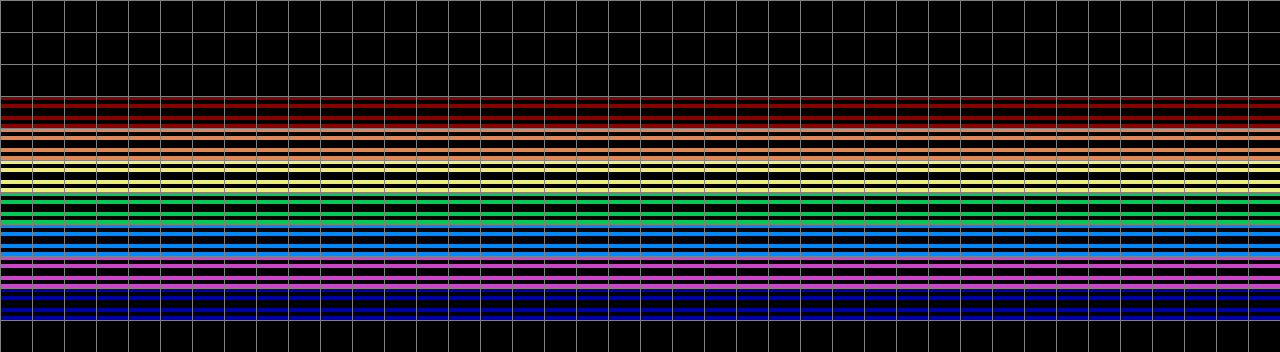
\includegraphics[width=13cm]{titlescreen/titlescreen_colour_only_grid.png}%
    \end{adjustbox}
  \caption{The section of the screen with our stripes painted.}
\end{figure}

\subsection{Drawing the Text}

Next up is to write out the title screen\index{screen}'s text to \icode{SCREEN\_RAM}. This we do in \icode{DrawTitleScreenText\index{DrawTitleScreenText}}
using a similar loop to \icode{DrawStripesBehindTitle\index{DrawStripesBehindTitle}}. 

\begin{lstlisting}[caption=In \icode{DrawTitleScreenText\index{DrawTitleScreenText}},escapechar=\%]
DrawTitleTextLoop%\index{DrawTitleTextLoop}%   
        LDA titleScreenTextLine1%\index{titleScreenTextLine1}% - $01,X
        AND #ASCII_BITMASK%\index{ASCII\_BITMASK}%
        STA SCREEN_RAM%\index{SCREEN\_RAM}% + LINE11_COL39%\index{LINE11\_COL39}%,X
        LDA titleScreenTextLine2%\index{titleScreenTextLine2}% - $01,X
        AND #ASCII_BITMASK%\index{ASCII\_BITMASK}%
        STA SCREEN_RAM%\index{SCREEN\_RAM}% + LINE13_COL39%\index{LINE13\_COL39}%,X
        LDA titleScreenTextLine3%\index{titleScreenTextLine3}% - $01,X
        AND #ASCII_BITMASK%\index{ASCII\_BITMASK}%
        STA SCREEN_RAM%\index{SCREEN\_RAM}% + LINE15_COL39%\index{LINE15\_COL39}%,X
        LDA titleScreenTextLine4%\index{titleScreenTextLine4}% - $01,X
        AND #ASCII_BITMASK%\index{ASCII\_BITMASK}%
        STA SCREEN_RAM%\index{SCREEN\_RAM}% + LINE17_COL39%\index{LINE17\_COL39}%,X
        LDA titleScreenTextLine5%\index{titleScreenTextLine5}% - $01,X
        AND #ASCII_BITMASK%\index{ASCII\_BITMASK}%
        STA SCREEN_RAM%\index{SCREEN\_RAM}% + LINE19_COL39%\index{LINE19\_COL39}%,X

        LDA #GRAY2
        STA COLOR_RAM%\index{COLOR\_RAM}% + LINE11_COL39%\index{LINE11\_COL39}%,X
        STA COLOR_RAM%\index{COLOR\_RAM}% + LINE13_COL39%\index{LINE13\_COL39}%,X
        STA COLOR_RAM%\index{COLOR\_RAM}% + LINE15_COL39%\index{LINE15\_COL39}%,X
        STA COLOR_RAM%\index{COLOR\_RAM}% + LINE17_COL39%\index{LINE17\_COL39}%,X
        STA COLOR_RAM%\index{COLOR\_RAM}% + LINE19_COL39%\index{LINE19\_COL39}%,X
        DEX
        BNE DrawTitleTextLoop%\index{DrawTitleTextLoop}%
\end{lstlisting}

In this case we're not writing a single character\index{character} over and over, rather we're writing text we've defined elsewhere
in variables \icode{titleScreenTextLine[1-5]}:

\begin{lstlisting}[caption=In \icode{DrawTitleScreenText\index{DrawTitleScreenText}},escapechar=\%]
titleScreenTextLine1%\index{titleScreenTextLine1}%  .TEXT "IRIDIS ALPHA.....  HARD AND FAST ZAPPING%\index{ZAPPING}%"
titleScreenTextLine2%\index{titleScreenTextLine2}%  .TEXT "PRESS FIRE TO BEGIN PLAY.. ONCE STARTED%\index{STARTED}%,"
titleScreenTextLine3%\index{titleScreenTextLine3}%  .TEXT "F1 FOR PAUSE MODE     Q TO QUIT THE GAME"
titleScreenTextLine4%\index{titleScreenTextLine4}%  .TEXT "CREATED BY JEFF MINTER...SPACE EASY/HARD"
titleScreenTextLine5%\index{titleScreenTextLine5}%  .TEXT "LAST GILBY HIT 0000000; MODE IS NOW EASY"
\end{lstlisting}

In each iteration of the loop we write a character\index{character} to all five columns, plucking it from the position in
\icode{titleScreenTextLine[1-5]} given by \icode{X}. 

\begin{figure}[H]
  {
    \setlength{\tabcolsep}{3.0pt}
    \setlength\cmidrulewidth{\heavyrulewidth} % Make cmidrule = 
    \begin{adjustbox}{width=13cm,center}
      \begin{tikzpicture}
    \fill[gray] (0,4) rectangle ++ (1,1);
    \fill[gray] (1,4) rectangle ++ (1,1);
    \fill[gray] (2,4) rectangle ++ (1,1);
    \fill[gray] (3,4) rectangle ++ (1,1);
    \fill[gray] (5,4) rectangle ++ (1,1);
    \fill[gray] (6,4) rectangle ++ (1,1);
    \fill[gray] (7,4) rectangle ++ (1,1);
    \fill[gray] (8,4) rectangle ++ (1,1);
    \fill[gray] (9,4) rectangle ++ (1,1);
    \fill[gray] (11,4) rectangle ++ (1,1);
    \fill[gray] (12,4) rectangle ++ (1,1);
    \fill[gray] (13,4) rectangle ++ (1,1);
    \fill[gray] (15,4) rectangle ++ (1,1);
    \fill[gray] (16,4) rectangle ++ (1,1);
    \fill[gray] (17,4) rectangle ++ (1,1);
    \fill[gray] (18,4) rectangle ++ (1,1);
    \fill[gray] (19,4) rectangle ++ (1,1);
    \fill[gray] (20,4) rectangle ++ (1,1);
    \fill[gray] (21,4) rectangle ++ (1,1);
    \fill[gray] (22,4) rectangle ++ (1,1);
    \fill[gray] (24,4) rectangle ++ (1,1);
    \fill[gray] (25,4) rectangle ++ (1,1);
    \fill[gray] (26,4) rectangle ++ (1,1);
    \fill[gray] (27,4) rectangle ++ (1,1);
    \fill[gray] (29,4) rectangle ++ (1,1);
    \fill[gray] (30,4) rectangle ++ (1,1);
    \fill[gray] (32,4) rectangle ++ (1,1);
    \fill[gray] (33,4) rectangle ++ (1,1);
    \fill[gray] (34,4) rectangle ++ (1,1);
    \fill[gray] (36,4) rectangle ++ (1,1);
    \fill[gray] (37,4) rectangle ++ (1,1);
    \fill[gray] (38,4) rectangle ++ (1,1);
    \fill[gray] (39,4) rectangle ++ (1,1);
    \fill[gray] (0,6) rectangle ++ (1,1);
    \fill[gray] (1,6) rectangle ++ (1,1);
    \fill[gray] (2,6) rectangle ++ (1,1);
    \fill[gray] (3,6) rectangle ++ (1,1);
    \fill[gray] (4,6) rectangle ++ (1,1);
    \fill[gray] (5,6) rectangle ++ (1,1);
    \fill[gray] (6,6) rectangle ++ (1,1);
    \fill[gray] (8,6) rectangle ++ (1,1);
    \fill[gray] (9,6) rectangle ++ (1,1);
    \fill[gray] (11,6) rectangle ++ (1,1);
    \fill[gray] (12,6) rectangle ++ (1,1);
    \fill[gray] (13,6) rectangle ++ (1,1);
    \fill[gray] (14,6) rectangle ++ (1,1);
    \fill[gray] (16,6) rectangle ++ (1,1);
    \fill[gray] (17,6) rectangle ++ (1,1);
    \fill[gray] (18,6) rectangle ++ (1,1);
    \fill[gray] (19,6) rectangle ++ (1,1);
    \fill[gray] (20,6) rectangle ++ (1,1);
    \fill[gray] (21,6) rectangle ++ (1,1);
    \fill[gray] (22,6) rectangle ++ (1,1);
    \fill[gray] (23,6) rectangle ++ (1,1);
    \fill[gray] (24,6) rectangle ++ (1,1);
    \fill[gray] (25,6) rectangle ++ (1,1);
    \fill[gray] (26,6) rectangle ++ (1,1);
    \fill[gray] (27,6) rectangle ++ (1,1);
    \fill[gray] (28,6) rectangle ++ (1,1);
    \fill[gray] (29,6) rectangle ++ (1,1);
    \fill[gray] (31,6) rectangle ++ (1,1);
    \fill[gray] (32,6) rectangle ++ (1,1);
    \fill[gray] (33,6) rectangle ++ (1,1);
    \fill[gray] (34,6) rectangle ++ (1,1);
    \fill[gray] (35,6) rectangle ++ (1,1);
    \fill[gray] (36,6) rectangle ++ (1,1);
    \fill[gray] (37,6) rectangle ++ (1,1);
    \fill[gray] (38,6) rectangle ++ (1,1);
    \fill[gray] (39,6) rectangle ++ (1,1);
    \fill[gray] (0,8) rectangle ++ (1,1);
    \fill[gray] (1,8) rectangle ++ (1,1);
    \fill[gray] (3,8) rectangle ++ (1,1);
    \fill[gray] (4,8) rectangle ++ (1,1);
    \fill[gray] (5,8) rectangle ++ (1,1);
    \fill[gray] (7,8) rectangle ++ (1,1);
    \fill[gray] (8,8) rectangle ++ (1,1);
    \fill[gray] (9,8) rectangle ++ (1,1);
    \fill[gray] (10,8) rectangle ++ (1,1);
    \fill[gray] (11,8) rectangle ++ (1,1);
    \fill[gray] (13,8) rectangle ++ (1,1);
    \fill[gray] (14,8) rectangle ++ (1,1);
    \fill[gray] (15,8) rectangle ++ (1,1);
    \fill[gray] (16,8) rectangle ++ (1,1);
    \fill[gray] (22,8) rectangle ++ (1,1);
    \fill[gray] (24,8) rectangle ++ (1,1);
    \fill[gray] (25,8) rectangle ++ (1,1);
    \fill[gray] (27,8) rectangle ++ (1,1);
    \fill[gray] (28,8) rectangle ++ (1,1);
    \fill[gray] (29,8) rectangle ++ (1,1);
    \fill[gray] (30,8) rectangle ++ (1,1);
    \fill[gray] (32,8) rectangle ++ (1,1);
    \fill[gray] (33,8) rectangle ++ (1,1);
    \fill[gray] (34,8) rectangle ++ (1,1);
    \fill[gray] (36,8) rectangle ++ (1,1);
    \fill[gray] (37,8) rectangle ++ (1,1);
    \fill[gray] (38,8) rectangle ++ (1,1);
    \fill[gray] (39,8) rectangle ++ (1,1);
    \fill[gray] (0,10) rectangle ++ (1,1);
    \fill[gray] (1,10) rectangle ++ (1,1);
    \fill[gray] (2,10) rectangle ++ (1,1);
    \fill[gray] (3,10) rectangle ++ (1,1);
    \fill[gray] (4,10) rectangle ++ (1,1);
    \fill[gray] (6,10) rectangle ++ (1,1);
    \fill[gray] (7,10) rectangle ++ (1,1);
    \fill[gray] (8,10) rectangle ++ (1,1);
    \fill[gray] (9,10) rectangle ++ (1,1);
    \fill[gray] (11,10) rectangle ++ (1,1);
    \fill[gray] (12,10) rectangle ++ (1,1);
    \fill[gray] (14,10) rectangle ++ (1,1);
    \fill[gray] (15,10) rectangle ++ (1,1);
    \fill[gray] (16,10) rectangle ++ (1,1);
    \fill[gray] (17,10) rectangle ++ (1,1);
    \fill[gray] (18,10) rectangle ++ (1,1);
    \fill[gray] (20,10) rectangle ++ (1,1);
    \fill[gray] (21,10) rectangle ++ (1,1);
    \fill[gray] (22,10) rectangle ++ (1,1);
    \fill[gray] (23,10) rectangle ++ (1,1);
    \fill[gray] (24,10) rectangle ++ (1,1);
    \fill[gray] (25,10) rectangle ++ (1,1);
    \fill[gray] (27,10) rectangle ++ (1,1);
    \fill[gray] (28,10) rectangle ++ (1,1);
    \fill[gray] (29,10) rectangle ++ (1,1);
    \fill[gray] (30,10) rectangle ++ (1,1);
    \fill[gray] (32,10) rectangle ++ (1,1);
    \fill[gray] (33,10) rectangle ++ (1,1);
    \fill[gray] (34,10) rectangle ++ (1,1);
    \fill[gray] (35,10) rectangle ++ (1,1);
    \fill[gray] (36,10) rectangle ++ (1,1);
    \fill[gray] (37,10) rectangle ++ (1,1);
    \fill[gray] (38,10) rectangle ++ (1,1);
    \fill[gray] (39,10) rectangle ++ (1,1);
    \fill[gray] (0,12) rectangle ++ (1,1);
    \fill[gray] (1,12) rectangle ++ (1,1);
    \fill[gray] (2,12) rectangle ++ (1,1);
    \fill[gray] (3,12) rectangle ++ (1,1);
    \fill[gray] (4,12) rectangle ++ (1,1);
    \fill[gray] (5,12) rectangle ++ (1,1);
    \fill[gray] (7,12) rectangle ++ (1,1);
    \fill[gray] (8,12) rectangle ++ (1,1);
    \fill[gray] (9,12) rectangle ++ (1,1);
    \fill[gray] (10,12) rectangle ++ (1,1);
    \fill[gray] (11,12) rectangle ++ (1,1);
    \fill[gray] (12,12) rectangle ++ (1,1);
    \fill[gray] (13,12) rectangle ++ (1,1);
    \fill[gray] (14,12) rectangle ++ (1,1);
    \fill[gray] (15,12) rectangle ++ (1,1);
    \fill[gray] (16,12) rectangle ++ (1,1);
    \fill[gray] (19,12) rectangle ++ (1,1);
    \fill[gray] (20,12) rectangle ++ (1,1);
    \fill[gray] (21,12) rectangle ++ (1,1);
    \fill[gray] (22,12) rectangle ++ (1,1);
    \fill[gray] (24,12) rectangle ++ (1,1);
    \fill[gray] (25,12) rectangle ++ (1,1);
    \fill[gray] (26,12) rectangle ++ (1,1);
    \fill[gray] (28,12) rectangle ++ (1,1);
    \fill[gray] (29,12) rectangle ++ (1,1);
    \fill[gray] (30,12) rectangle ++ (1,1);
    \fill[gray] (31,12) rectangle ++ (1,1);
    \fill[gray] (33,12) rectangle ++ (1,1);
    \fill[gray] (34,12) rectangle ++ (1,1);
    \fill[gray] (35,12) rectangle ++ (1,1);
    \fill[gray] (36,12) rectangle ++ (1,1);
    \fill[gray] (37,12) rectangle ++ (1,1);
    \fill[gray] (38,12) rectangle ++ (1,1);
    \fill[gray] (39,12) rectangle ++ (1,1);
    \fill[gray] (0,15) rectangle ++ (1,1);
    \fill[gray] (1,15) rectangle ++ (1,1);
    \fill[gray] (2,15) rectangle ++ (1,1);
    \fill[gray] (3,15) rectangle ++ (1,1);
    \fill[gray] (4,15) rectangle ++ (1,1);
    \fill[gray] (5,15) rectangle ++ (1,1);
    \fill[gray] (6,15) rectangle ++ (1,1);
    \fill[gray] (7,15) rectangle ++ (1,1);
    \fill[gray] (8,15) rectangle ++ (1,1);
    \fill[gray] (9,15) rectangle ++ (1,1);
    \fill[gray] (10,15) rectangle ++ (1,1);
    \fill[gray] (11,15) rectangle ++ (1,1);
    \fill[gray] (12,15) rectangle ++ (1,1);
    \fill[gray] (13,15) rectangle ++ (1,1);
    \fill[gray] (14,15) rectangle ++ (1,1);
    \fill[gray] (15,15) rectangle ++ (1,1);
    \fill[gray] (16,15) rectangle ++ (1,1);
    \fill[gray] (17,15) rectangle ++ (1,1);
    \fill[gray] (18,15) rectangle ++ (1,1);
    \fill[gray] (19,15) rectangle ++ (1,1);
    \fill[gray] (20,15) rectangle ++ (1,1);
    \fill[gray] (21,15) rectangle ++ (1,1);
    \fill[gray] (22,15) rectangle ++ (1,1);
    \fill[gray] (23,15) rectangle ++ (1,1);
    \fill[gray] (24,15) rectangle ++ (1,1);
    \fill[gray] (25,15) rectangle ++ (1,1);
    \fill[gray] (26,15) rectangle ++ (1,1);
    \fill[gray] (27,15) rectangle ++ (1,1);
    \fill[gray] (28,15) rectangle ++ (1,1);
    \fill[gray] (29,15) rectangle ++ (1,1);
    \fill[gray] (30,15) rectangle ++ (1,1);
    \fill[gray] (31,15) rectangle ++ (1,1);
    \fill[gray] (32,15) rectangle ++ (1,1);
    \fill[gray] (33,15) rectangle ++ (1,1);
    \fill[gray] (34,15) rectangle ++ (1,1);
    \fill[gray] (35,15) rectangle ++ (1,1);
    \fill[gray] (36,15) rectangle ++ (1,1);
    \fill[gray] (37,15) rectangle ++ (1,1);
    \fill[gray] (38,15) rectangle ++ (1,1);
    \fill[gray] (39,15) rectangle ++ (1,1);
    \fill[gray] (0,16) rectangle ++ (1,1);
    \fill[gray] (1,16) rectangle ++ (1,1);
    \fill[gray] (2,16) rectangle ++ (1,1);
    \fill[gray] (3,16) rectangle ++ (1,1);
    \fill[gray] (4,16) rectangle ++ (1,1);
    \fill[gray] (5,16) rectangle ++ (1,1);
    \fill[gray] (6,16) rectangle ++ (1,1);
    \fill[gray] (7,16) rectangle ++ (1,1);
    \fill[gray] (8,16) rectangle ++ (1,1);
    \fill[gray] (9,16) rectangle ++ (1,1);
    \fill[gray] (10,16) rectangle ++ (1,1);
    \fill[gray] (11,16) rectangle ++ (1,1);
    \fill[gray] (12,16) rectangle ++ (1,1);
    \fill[gray] (13,16) rectangle ++ (1,1);
    \fill[gray] (14,16) rectangle ++ (1,1);
    \fill[gray] (15,16) rectangle ++ (1,1);
    \fill[gray] (16,16) rectangle ++ (1,1);
    \fill[gray] (17,16) rectangle ++ (1,1);
    \fill[gray] (18,16) rectangle ++ (1,1);
    \fill[gray] (19,16) rectangle ++ (1,1);
    \fill[gray] (20,16) rectangle ++ (1,1);
    \fill[gray] (21,16) rectangle ++ (1,1);
    \fill[gray] (22,16) rectangle ++ (1,1);
    \fill[gray] (23,16) rectangle ++ (1,1);
    \fill[gray] (24,16) rectangle ++ (1,1);
    \fill[gray] (25,16) rectangle ++ (1,1);
    \fill[gray] (26,16) rectangle ++ (1,1);
    \fill[gray] (27,16) rectangle ++ (1,1);
    \fill[gray] (28,16) rectangle ++ (1,1);
    \fill[gray] (29,16) rectangle ++ (1,1);
    \fill[gray] (30,16) rectangle ++ (1,1);
    \fill[gray] (31,16) rectangle ++ (1,1);
    \fill[gray] (32,16) rectangle ++ (1,1);
    \fill[gray] (33,16) rectangle ++ (1,1);
    \fill[gray] (34,16) rectangle ++ (1,1);
    \fill[gray] (35,16) rectangle ++ (1,1);
    \fill[gray] (36,16) rectangle ++ (1,1);
    \fill[gray] (37,16) rectangle ++ (1,1);
    \fill[gray] (38,16) rectangle ++ (1,1);
    \fill[gray] (39,16) rectangle ++ (1,1);
    \fill[gray] (0,17) rectangle ++ (1,1);
    \fill[gray] (1,17) rectangle ++ (1,1);
    \fill[gray] (2,17) rectangle ++ (1,1);
    \fill[gray] (3,17) rectangle ++ (1,1);
    \fill[gray] (4,17) rectangle ++ (1,1);
    \fill[gray] (5,17) rectangle ++ (1,1);
    \fill[gray] (6,17) rectangle ++ (1,1);
    \fill[gray] (7,17) rectangle ++ (1,1);
    \fill[gray] (8,17) rectangle ++ (1,1);
    \fill[gray] (9,17) rectangle ++ (1,1);
    \fill[gray] (10,17) rectangle ++ (1,1);
    \fill[gray] (11,17) rectangle ++ (1,1);
    \fill[gray] (12,17) rectangle ++ (1,1);
    \fill[gray] (13,17) rectangle ++ (1,1);
    \fill[gray] (14,17) rectangle ++ (1,1);
    \fill[gray] (15,17) rectangle ++ (1,1);
    \fill[gray] (16,17) rectangle ++ (1,1);
    \fill[gray] (17,17) rectangle ++ (1,1);
    \fill[gray] (18,17) rectangle ++ (1,1);
    \fill[gray] (19,17) rectangle ++ (1,1);
    \fill[gray] (20,17) rectangle ++ (1,1);
    \fill[gray] (21,17) rectangle ++ (1,1);
    \fill[gray] (22,17) rectangle ++ (1,1);
    \fill[gray] (23,17) rectangle ++ (1,1);
    \fill[gray] (24,17) rectangle ++ (1,1);
    \fill[gray] (25,17) rectangle ++ (1,1);
    \fill[gray] (26,17) rectangle ++ (1,1);
    \fill[gray] (27,17) rectangle ++ (1,1);
    \fill[gray] (28,17) rectangle ++ (1,1);
    \fill[gray] (29,17) rectangle ++ (1,1);
    \fill[gray] (30,17) rectangle ++ (1,1);
    \fill[gray] (31,17) rectangle ++ (1,1);
    \fill[gray] (32,17) rectangle ++ (1,1);
    \fill[gray] (33,17) rectangle ++ (1,1);
    \fill[gray] (34,17) rectangle ++ (1,1);
    \fill[gray] (35,17) rectangle ++ (1,1);
    \fill[gray] (36,17) rectangle ++ (1,1);
    \fill[gray] (37,17) rectangle ++ (1,1);
    \fill[gray] (38,17) rectangle ++ (1,1);
    \fill[gray] (39,17) rectangle ++ (1,1);
    \fill[gray] (0,18) rectangle ++ (1,1);
    \fill[gray] (1,18) rectangle ++ (1,1);
    \fill[gray] (2,18) rectangle ++ (1,1);
    \fill[gray] (3,18) rectangle ++ (1,1);
    \fill[gray] (4,18) rectangle ++ (1,1);
    \fill[gray] (5,18) rectangle ++ (1,1);
    \fill[gray] (6,18) rectangle ++ (1,1);
    \fill[gray] (7,18) rectangle ++ (1,1);
    \fill[gray] (8,18) rectangle ++ (1,1);
    \fill[gray] (9,18) rectangle ++ (1,1);
    \fill[gray] (10,18) rectangle ++ (1,1);
    \fill[gray] (11,18) rectangle ++ (1,1);
    \fill[gray] (12,18) rectangle ++ (1,1);
    \fill[gray] (13,18) rectangle ++ (1,1);
    \fill[gray] (14,18) rectangle ++ (1,1);
    \fill[gray] (15,18) rectangle ++ (1,1);
    \fill[gray] (16,18) rectangle ++ (1,1);
    \fill[gray] (17,18) rectangle ++ (1,1);
    \fill[gray] (18,18) rectangle ++ (1,1);
    \fill[gray] (19,18) rectangle ++ (1,1);
    \fill[gray] (20,18) rectangle ++ (1,1);
    \fill[gray] (21,18) rectangle ++ (1,1);
    \fill[gray] (22,18) rectangle ++ (1,1);
    \fill[gray] (23,18) rectangle ++ (1,1);
    \fill[gray] (24,18) rectangle ++ (1,1);
    \fill[gray] (25,18) rectangle ++ (1,1);
    \fill[gray] (26,18) rectangle ++ (1,1);
    \fill[gray] (27,18) rectangle ++ (1,1);
    \fill[gray] (28,18) rectangle ++ (1,1);
    \fill[gray] (29,18) rectangle ++ (1,1);
    \fill[gray] (30,18) rectangle ++ (1,1);
    \fill[gray] (31,18) rectangle ++ (1,1);
    \fill[gray] (32,18) rectangle ++ (1,1);
    \fill[gray] (33,18) rectangle ++ (1,1);
    \fill[gray] (34,18) rectangle ++ (1,1);
    \fill[gray] (35,18) rectangle ++ (1,1);
    \fill[gray] (36,18) rectangle ++ (1,1);
    \fill[gray] (37,18) rectangle ++ (1,1);
    \fill[gray] (38,18) rectangle ++ (1,1);
    \fill[gray] (39,18) rectangle ++ (1,1);
    \fill[gray] (0,19) rectangle ++ (1,1);
    \fill[gray] (1,19) rectangle ++ (1,1);
    \fill[gray] (2,19) rectangle ++ (1,1);
    \fill[gray] (3,19) rectangle ++ (1,1);
    \fill[gray] (4,19) rectangle ++ (1,1);
    \fill[gray] (5,19) rectangle ++ (1,1);
    \fill[gray] (6,19) rectangle ++ (1,1);
    \fill[gray] (7,19) rectangle ++ (1,1);
    \fill[gray] (8,19) rectangle ++ (1,1);
    \fill[gray] (9,19) rectangle ++ (1,1);
    \fill[gray] (10,19) rectangle ++ (1,1);
    \fill[gray] (11,19) rectangle ++ (1,1);
    \fill[gray] (12,19) rectangle ++ (1,1);
    \fill[gray] (13,19) rectangle ++ (1,1);
    \fill[gray] (14,19) rectangle ++ (1,1);
    \fill[gray] (15,19) rectangle ++ (1,1);
    \fill[gray] (16,19) rectangle ++ (1,1);
    \fill[gray] (17,19) rectangle ++ (1,1);
    \fill[gray] (18,19) rectangle ++ (1,1);
    \fill[gray] (19,19) rectangle ++ (1,1);
    \fill[gray] (20,19) rectangle ++ (1,1);
    \fill[gray] (21,19) rectangle ++ (1,1);
    \fill[gray] (22,19) rectangle ++ (1,1);
    \fill[gray] (23,19) rectangle ++ (1,1);
    \fill[gray] (24,19) rectangle ++ (1,1);
    \fill[gray] (25,19) rectangle ++ (1,1);
    \fill[gray] (26,19) rectangle ++ (1,1);
    \fill[gray] (27,19) rectangle ++ (1,1);
    \fill[gray] (28,19) rectangle ++ (1,1);
    \fill[gray] (29,19) rectangle ++ (1,1);
    \fill[gray] (30,19) rectangle ++ (1,1);
    \fill[gray] (31,19) rectangle ++ (1,1);
    \fill[gray] (32,19) rectangle ++ (1,1);
    \fill[gray] (33,19) rectangle ++ (1,1);
    \fill[gray] (34,19) rectangle ++ (1,1);
    \fill[gray] (35,19) rectangle ++ (1,1);
    \fill[gray] (36,19) rectangle ++ (1,1);
    \fill[gray] (37,19) rectangle ++ (1,1);
    \fill[gray] (38,19) rectangle ++ (1,1);
    \fill[gray] (39,19) rectangle ++ (1,1);
    \fill[gray] (0,20) rectangle ++ (1,1);
    \fill[gray] (1,20) rectangle ++ (1,1);
    \fill[gray] (2,20) rectangle ++ (1,1);
    \fill[gray] (3,20) rectangle ++ (1,1);
    \fill[gray] (4,20) rectangle ++ (1,1);
    \fill[gray] (5,20) rectangle ++ (1,1);
    \fill[gray] (6,20) rectangle ++ (1,1);
    \fill[gray] (7,20) rectangle ++ (1,1);
    \fill[gray] (8,20) rectangle ++ (1,1);
    \fill[gray] (9,20) rectangle ++ (1,1);
    \fill[gray] (10,20) rectangle ++ (1,1);
    \fill[gray] (11,20) rectangle ++ (1,1);
    \fill[gray] (12,20) rectangle ++ (1,1);
    \fill[gray] (13,20) rectangle ++ (1,1);
    \fill[gray] (14,20) rectangle ++ (1,1);
    \fill[gray] (15,20) rectangle ++ (1,1);
    \fill[gray] (16,20) rectangle ++ (1,1);
    \fill[gray] (17,20) rectangle ++ (1,1);
    \fill[gray] (18,20) rectangle ++ (1,1);
    \fill[gray] (19,20) rectangle ++ (1,1);
    \fill[gray] (20,20) rectangle ++ (1,1);
    \fill[gray] (21,20) rectangle ++ (1,1);
    \fill[gray] (22,20) rectangle ++ (1,1);
    \fill[gray] (23,20) rectangle ++ (1,1);
    \fill[gray] (24,20) rectangle ++ (1,1);
    \fill[gray] (25,20) rectangle ++ (1,1);
    \fill[gray] (26,20) rectangle ++ (1,1);
    \fill[gray] (27,20) rectangle ++ (1,1);
    \fill[gray] (28,20) rectangle ++ (1,1);
    \fill[gray] (29,20) rectangle ++ (1,1);
    \fill[gray] (30,20) rectangle ++ (1,1);
    \fill[gray] (31,20) rectangle ++ (1,1);
    \fill[gray] (32,20) rectangle ++ (1,1);
    \fill[gray] (33,20) rectangle ++ (1,1);
    \fill[gray] (34,20) rectangle ++ (1,1);
    \fill[gray] (35,20) rectangle ++ (1,1);
    \fill[gray] (36,20) rectangle ++ (1,1);
    \fill[gray] (37,20) rectangle ++ (1,1);
    \fill[gray] (38,20) rectangle ++ (1,1);
    \fill[gray] (39,20) rectangle ++ (1,1);
    \fill[gray] (0,21) rectangle ++ (1,1);
    \fill[gray] (1,21) rectangle ++ (1,1);
    \fill[gray] (2,21) rectangle ++ (1,1);
    \fill[gray] (3,21) rectangle ++ (1,1);
    \fill[gray] (4,21) rectangle ++ (1,1);
    \fill[gray] (5,21) rectangle ++ (1,1);
    \fill[gray] (6,21) rectangle ++ (1,1);
    \fill[gray] (7,21) rectangle ++ (1,1);
    \fill[gray] (8,21) rectangle ++ (1,1);
    \fill[gray] (9,21) rectangle ++ (1,1);
    \fill[gray] (10,21) rectangle ++ (1,1);
    \fill[gray] (11,21) rectangle ++ (1,1);
    \fill[gray] (12,21) rectangle ++ (1,1);
    \fill[gray] (13,21) rectangle ++ (1,1);
    \fill[gray] (14,21) rectangle ++ (1,1);
    \fill[gray] (15,21) rectangle ++ (1,1);
    \fill[gray] (16,21) rectangle ++ (1,1);
    \fill[gray] (17,21) rectangle ++ (1,1);
    \fill[gray] (18,21) rectangle ++ (1,1);
    \fill[gray] (19,21) rectangle ++ (1,1);
    \fill[gray] (20,21) rectangle ++ (1,1);
    \fill[gray] (21,21) rectangle ++ (1,1);
    \fill[gray] (22,21) rectangle ++ (1,1);
    \fill[gray] (23,21) rectangle ++ (1,1);
    \fill[gray] (24,21) rectangle ++ (1,1);
    \fill[gray] (25,21) rectangle ++ (1,1);
    \fill[gray] (26,21) rectangle ++ (1,1);
    \fill[gray] (27,21) rectangle ++ (1,1);
    \fill[gray] (28,21) rectangle ++ (1,1);
    \fill[gray] (29,21) rectangle ++ (1,1);
    \fill[gray] (30,21) rectangle ++ (1,1);
    \fill[gray] (31,21) rectangle ++ (1,1);
    \fill[gray] (32,21) rectangle ++ (1,1);
    \fill[gray] (33,21) rectangle ++ (1,1);
    \fill[gray] (34,21) rectangle ++ (1,1);
    \fill[gray] (35,21) rectangle ++ (1,1);
    \fill[gray] (36,21) rectangle ++ (1,1);
    \fill[gray] (37,21) rectangle ++ (1,1);
    \fill[gray] (38,21) rectangle ++ (1,1);
    \fill[gray] (39,21) rectangle ++ (1,1);  
        \draw[step=1.0,gray,thin] (0,0) grid (40,25);
        \node[matrix of math nodes,anchor=south west,inner sep=0pt,
              nodes={draw,minimum size=1cm,anchor=center},
              column sep=-\pgflinewidth,row sep=-\pgflinewidth,font=\huge\ttfamily]
              {
\icode{20} & \icode{20} & \icode{20} & \icode{20} & \icode{20} & \icode{20} & \icode{20} & \icode{20} & \icode{20} & \icode{20} & \icode{20} & \icode{20} & \icode{20} & \icode{20} & \icode{20} & \icode{20} & \icode{20} & \icode{20} & \icode{20} & \icode{20} & \icode{20} & \icode{20} & \icode{20} & \icode{20} & \icode{20} & \icode{20} & \icode{20} &
\icode{20} & \icode{20} & \icode{20} & \icode{20} & \icode{20} & \icode{20} & \icode{20} & \icode{20} & \icode{20} & \icode{20} & \icode{20} & \icode{20} & \icode{20} \\
\icode{20} & \icode{20} & \icode{20} & \icode{20} & \icode{20} & \icode{20} & \icode{20} & \icode{20} & \icode{20} & \icode{20} & \icode{20} & \icode{20} & \icode{20} & \icode{20} & \icode{20} & \icode{20} & \icode{20} & \icode{20} & \icode{20} & \icode{20} & \icode{20} & \icode{20} & \icode{20} & \icode{20} & \icode{20} & \icode{20} & \icode{20} &
\icode{20} & \icode{20} & \icode{20} & \icode{20} & \icode{20} & \icode{20} & \icode{20} & \icode{20} & \icode{20} & \icode{20} & \icode{20} & \icode{20} & \icode{20} \\
\icode{20} & \icode{20} & \icode{20} & \icode{20} & \icode{20} & \icode{20} & \icode{20} & \icode{20} & \icode{20} & \icode{20} & \icode{20} & \icode{20} & \icode{20} & \icode{20} & \icode{20} & \icode{20} & \icode{20} & \icode{20} & \icode{20} & \icode{20} & \icode{20} & \icode{20} & \icode{20} & \icode{20} & \icode{20} & \icode{20} & \icode{20} &
\icode{20} & \icode{20} & \icode{20} & \icode{20} & \icode{20} & \icode{20} & \icode{20} & \icode{20} & \icode{20} & \icode{20} & \icode{20} & \icode{20} & \icode{20} \\
\icode{00} & \icode{00} & \icode{00} & \icode{00} & \icode{00} & \icode{00} & \icode{00} & \icode{00} & \icode{00} & \icode{00} & \icode{00} & \icode{00} & \icode{00} & \icode{00} & \icode{00} & \icode{00} & \icode{00} & \icode{00} & \icode{00} & \icode{00} & \icode{00} & \icode{00} & \icode{00} & \icode{00} & \icode{00} & \icode{00} & \icode{00} &
\icode{00} & \icode{00} & \icode{00} & \icode{00} & \icode{00} & \icode{00} & \icode{00} & \icode{00} & \icode{00} & \icode{00} & \icode{00} & \icode{00} & \icode{00} \\
\icode{00} & \icode{00} & \icode{00} & \icode{00} & \icode{00} & \icode{00} & \icode{00} & \icode{00} & \icode{00} & \icode{00} & \icode{00} & \icode{00} & \icode{00} & \icode{00} & \icode{00} & \icode{00} & \icode{00} & \icode{00} & \icode{00} & \icode{00} & \icode{00} & \icode{00} & \icode{00} & \icode{00} & \icode{00} & \icode{00} & \icode{00} &
\icode{00} & \icode{00} & \icode{00} & \icode{00} & \icode{00} & \icode{00} & \icode{00} & \icode{00} & \icode{00} & \icode{00} & \icode{00} & \icode{00} & \icode{00} \\
\icode{00} & \icode{00} & \icode{00} & \icode{00} & \icode{00} & \icode{00} & \icode{00} & \icode{00} & \icode{00} & \icode{00} & \icode{00} & \icode{00} & \icode{00} & \icode{00} & \icode{00} & \icode{00} & \icode{00} & \icode{00} & \icode{00} & \icode{00} & \icode{00} & \icode{00} & \icode{00} & \icode{00} & \icode{00} & \icode{00} & \icode{00} &
\icode{00} & \icode{00} & \icode{00} & \icode{00} & \icode{00} & \icode{00} & \icode{00} & \icode{00} & \icode{00} & \icode{00} & \icode{00} & \icode{00} & \icode{00} \\
\icode{00} & \icode{00} & \icode{00} & \icode{00} & \icode{00} & \icode{00} & \icode{00} & \icode{00} & \icode{00} & \icode{00} & \icode{00} & \icode{00} & \icode{00} & \icode{00} & \icode{00} & \icode{00} & \icode{00} & \icode{00} & \icode{00} & \icode{00} & \icode{00} & \icode{00} & \icode{00} & \icode{00} & \icode{00} & \icode{00} & \icode{00} &
\icode{00} & \icode{00} & \icode{00} & \icode{00} & \icode{00} & \icode{00} & \icode{00} & \icode{00} & \icode{00} & \icode{00} & \icode{00} & \icode{00} & \icode{00} \\
\icode{00} & \icode{00} & \icode{00} & \icode{00} & \icode{00} & \icode{00} & \icode{00} & \icode{00} & \icode{00} & \icode{00} & \icode{00} & \icode{00} & \icode{00} & \icode{00} & \icode{00} & \icode{00} & \icode{00} & \icode{00} & \icode{00} & \icode{00} & \icode{00} & \icode{00} & \icode{00} & \icode{00} & \icode{00} & \icode{00} & \icode{00} &
\icode{00} & \icode{00} & \icode{00} & \icode{00} & \icode{00} & \icode{00} & \icode{00} & \icode{00} & \icode{00} & \icode{00} & \icode{00} & \icode{00} & \icode{00} \\
\icode{00} & \icode{00} & \icode{00} & \icode{00} & \icode{00} & \icode{00} & \icode{00} & \icode{00} & \icode{00} & \icode{00} & \icode{00} & \icode{00} & \icode{00} & \icode{00} & \icode{00} & \icode{00} & \icode{00} & \icode{00} & \icode{00} & \icode{00} & \icode{00} & \icode{00} & \icode{00} & \icode{00} & \icode{00} & \icode{00} & \icode{00} &
\icode{00} & \icode{00} & \icode{00} & \icode{00} & \icode{00} & \icode{00} & \icode{00} & \icode{00} & \icode{00} & \icode{00} & \icode{00} & \icode{00} & \icode{00} \\
\icode{00} & \icode{00} & \icode{00} & \icode{00} & \icode{00} & \icode{00} & \icode{00} & \icode{00} & \icode{00} & \icode{00} & \icode{00} & \icode{00} & \icode{00} & \icode{00} & \icode{00} & \icode{00} & \icode{00} & \icode{00} & \icode{00} & \icode{00} & \icode{00} & \icode{00} & \icode{00} & \icode{00} & \icode{00} & \icode{00} & \icode{00} &
\icode{00} & \icode{00} & \icode{00} & \icode{00} & \icode{00} & \icode{00} & \icode{00} & \icode{00} & \icode{00} & \icode{00} & \icode{00} & \icode{00} & \icode{00} \\
\icode{20} & \icode{20} & \icode{20} & \icode{20} & \icode{20} & \icode{20} & \icode{20} & \icode{20} & \icode{20} & \icode{20} & \icode{20} & \icode{20} & \icode{20} & \icode{20} & \icode{20} & \icode{20} & \icode{20} & \icode{20} & \icode{20} & \icode{20} & \icode{20} & \icode{20} & \icode{20} & \icode{20} & \icode{20} & \icode{20} & \icode{20} &
\icode{20} & \icode{20} & \icode{20} & \icode{20} & \icode{20} & \icode{20} & \icode{20} & \icode{20} & \icode{20} & \icode{20} & \icode{20} & \icode{20} & \icode{20} \\
\icode{20} & \icode{20} & \icode{20} & \icode{20} & \icode{20} & \icode{20} & \icode{20} & \icode{20} & \icode{20} & \icode{20} & \icode{20} & \icode{20} & \icode{20} & \icode{20} & \icode{20} & \icode{20} & \icode{20} & \icode{20} & \icode{20} & \icode{20} & \icode{20} & \icode{20} & \icode{20} & \icode{20} & \icode{20} & \icode{20} & \icode{20} &
\icode{20} & \icode{20} & \icode{20} & \icode{20} & \icode{20} & \icode{20} & \icode{20} & \icode{20} & \icode{20} & \icode{20} & \icode{20} & \icode{20} & \icode{20} \\
\icode{09} & \icode{12} & \icode{09} & \icode{04} & \icode{09} & \icode{13} & \icode{20} & \icode{01} & \icode{0C} & \icode{10} & \icode{08} & \icode{01} & \icode{2E} & \icode{2E} & \icode{2E} & \icode{2E} & \icode{2E} & \icode{20} & \icode{20} & \icode{08} & \icode{01} & \icode{12} & \icode{04} & \icode{20} & \icode{01} & \icode{0E} & \icode{04} &
\icode{20} & \icode{06} & \icode{01} & \icode{13} & \icode{14} & \icode{20} & \icode{1A} & \icode{01} & \icode{10} & \icode{10} & \icode{09} & \icode{0E} & \icode{07} \\
\icode{20} & \icode{20} & \icode{20} & \icode{20} & \icode{20} & \icode{20} & \icode{20} & \icode{20} & \icode{20} & \icode{20} & \icode{20} & \icode{20} & \icode{20} & \icode{20} & \icode{20} & \icode{20} & \icode{20} & \icode{20} & \icode{20} & \icode{20} & \icode{20} & \icode{20} & \icode{20} & \icode{20} & \icode{20} & \icode{20} & \icode{20} &
\icode{20} & \icode{20} & \icode{20} & \icode{20} & \icode{20} & \icode{20} & \icode{20} & \icode{20} & \icode{20} & \icode{20} & \icode{20} & \icode{20} & \icode{20} \\
\icode{10} & \icode{12} & \icode{05} & \icode{13} & \icode{13} & \icode{20} & \icode{06} & \icode{09} & \icode{12} & \icode{05} & \icode{20} & \icode{14} & \icode{0F} & \icode{20} & \icode{02} & \icode{05} & \icode{07} & \icode{09} & \icode{0E} & \icode{20} & \icode{10} & \icode{0C} & \icode{01} & \icode{19} & \icode{2E} & \icode{2E} & \icode{20} &
\icode{0F} & \icode{0E} & \icode{03} & \icode{05} & \icode{20} & \icode{13} & \icode{14} & \icode{01} & \icode{12} & \icode{14} & \icode{05} & \icode{04} & \icode{2C} \\
\icode{20} & \icode{20} & \icode{20} & \icode{20} & \icode{20} & \icode{20} & \icode{20} & \icode{20} & \icode{20} & \icode{20} & \icode{20} & \icode{20} & \icode{20} & \icode{20} & \icode{20} & \icode{20} & \icode{20} & \icode{20} & \icode{20} & \icode{20} & \icode{20} & \icode{20} & \icode{20} & \icode{20} & \icode{20} & \icode{20} & \icode{20} &
\icode{20} & \icode{20} & \icode{20} & \icode{20} & \icode{20} & \icode{20} & \icode{20} & \icode{20} & \icode{20} & \icode{20} & \icode{20} & \icode{20} & \icode{20} \\
\icode{06} & \icode{31} & \icode{20} & \icode{06} & \icode{0F} & \icode{12} & \icode{20} & \icode{10} & \icode{01} & \icode{15} & \icode{13} & \icode{05} & \icode{20} & \icode{0D} & \icode{0F} & \icode{04} & \icode{05} & \icode{20} & \icode{20} & \icode{20} & \icode{20} & \icode{20} & \icode{11} & \icode{20} & \icode{14} & \icode{0F} & \icode{20} &
\icode{11} & \icode{15} & \icode{09} & \icode{14} & \icode{20} & \icode{14} & \icode{08} & \icode{05} & \icode{20} & \icode{07} & \icode{01} & \icode{0D} & \icode{05} \\
\icode{20} & \icode{20} & \icode{20} & \icode{20} & \icode{20} & \icode{20} & \icode{20} & \icode{20} & \icode{20} & \icode{20} & \icode{20} & \icode{20} & \icode{20} & \icode{20} & \icode{20} & \icode{20} & \icode{20} & \icode{20} & \icode{20} & \icode{20} & \icode{20} & \icode{20} & \icode{20} & \icode{20} & \icode{20} & \icode{20} & \icode{20} &
\icode{20} & \icode{20} & \icode{20} & \icode{20} & \icode{20} & \icode{20} & \icode{20} & \icode{20} & \icode{20} & \icode{20} & \icode{20} & \icode{20} & \icode{20} \\
\icode{03} & \icode{12} & \icode{05} & \icode{01} & \icode{14} & \icode{05} & \icode{04} & \icode{20} & \icode{02} & \icode{19} & \icode{20} & \icode{0A} & \icode{05} & \icode{06} & \icode{06} & \icode{20} & \icode{0D} & \icode{09} & \icode{0E} & \icode{14} & \icode{05} & \icode{12} & \icode{2E} & \icode{2E} & \icode{2E} & \icode{13} & \icode{10} &
\icode{01} & \icode{03} & \icode{05} & \icode{20} & \icode{05} & \icode{01} & \icode{13} & \icode{19} & \icode{2F} & \icode{08} & \icode{01} & \icode{12} & \icode{04} \\
\icode{20} & \icode{20} & \icode{20} & \icode{20} & \icode{20} & \icode{20} & \icode{20} & \icode{20} & \icode{20} & \icode{20} & \icode{20} & \icode{20} & \icode{20} & \icode{20} & \icode{20} & \icode{20} & \icode{20} & \icode{20} & \icode{20} & \icode{20} & \icode{20} & \icode{20} & \icode{20} & \icode{20} & \icode{20} & \icode{20} & \icode{20} &
\icode{20} & \icode{20} & \icode{20} & \icode{20} & \icode{20} & \icode{20} & \icode{20} & \icode{20} & \icode{20} & \icode{20} & \icode{20} & \icode{20} & \icode{20} \\
\icode{0C} & \icode{01} & \icode{13} & \icode{14} & \icode{20} & \icode{07} & \icode{09} & \icode{0C} & \icode{02} & \icode{19} & \icode{20} & \icode{08} & \icode{09} & \icode{14} & \icode{20} & \icode{30} & \icode{30} & \icode{30} & \icode{30} & \icode{30} & \icode{30} & \icode{30} & \icode{3B} & \icode{20} & \icode{0D} & \icode{0F} & \icode{04} &
\icode{05} & \icode{20} & \icode{09} & \icode{13} & \icode{20} & \icode{0E} & \icode{0F} & \icode{17} & \icode{20} & \icode{05} & \icode{01} & \icode{13} & \icode{19} \\
\icode{20} & \icode{20} & \icode{20} & \icode{20} & \icode{20} & \icode{20} & \icode{20} & \icode{20} & \icode{20} & \icode{20} & \icode{20} & \icode{20} & \icode{20} & \icode{20} & \icode{20} & \icode{20} & \icode{20} & \icode{20} & \icode{20} & \icode{20} & \icode{20} & \icode{20} & \icode{20} & \icode{20} & \icode{20} & \icode{20} & \icode{20} &
\icode{20} & \icode{20} & \icode{20} & \icode{20} & \icode{20} & \icode{20} & \icode{20} & \icode{20} & \icode{20} & \icode{20} & \icode{20} & \icode{20} & \icode{20} \\
\icode{20} & \icode{20} & \icode{20} & \icode{20} & \icode{20} & \icode{20} & \icode{20} & \icode{20} & \icode{20} & \icode{20} & \icode{20} & \icode{20} & \icode{20} & \icode{20} & \icode{20} & \icode{20} & \icode{20} & \icode{20} & \icode{20} & \icode{20} & \icode{20} & \icode{20} & \icode{20} & \icode{20} & \icode{20} & \icode{20} & \icode{20} &
\icode{20} & \icode{20} & \icode{20} & \icode{20} & \icode{20} & \icode{20} & \icode{20} & \icode{20} & \icode{20} & \icode{20} & \icode{20} & \icode{20} & \icode{20} \\
\icode{20} & \icode{20} & \icode{20} & \icode{20} & \icode{20} & \icode{20} & \icode{20} & \icode{20} & \icode{20} & \icode{20} & \icode{20} & \icode{20} & \icode{20} & \icode{20} & \icode{20} & \icode{20} & \icode{20} & \icode{20} & \icode{20} & \icode{20} & \icode{20} & \icode{20} & \icode{20} & \icode{20} & \icode{20} & \icode{20} & \icode{20} &
\icode{20} & \icode{20} & \icode{20} & \icode{20} & \icode{20} & \icode{20} & \icode{20} & \icode{20} & \icode{20} & \icode{20} & \icode{20} & \icode{20} & \icode{20} \\
\icode{20} & \icode{20} & \icode{20} & \icode{20} & \icode{20} & \icode{20} & \icode{20} & \icode{20} & \icode{20} & \icode{20} & \icode{20} & \icode{20} & \icode{20} & \icode{20} & \icode{20} & \icode{20} & \icode{20} & \icode{20} & \icode{20} & \icode{20} & \icode{20} & \icode{20} & \icode{20} & \icode{20} & \icode{20} & \icode{20} & \icode{20} &
\icode{20} & \icode{20} & \icode{20} & \icode{20} & \icode{20} & \icode{20} & \icode{20} & \icode{20} & \icode{20} & \icode{20} & \icode{20} & \icode{20} & \icode{20} \\
						  };

      \end{tikzpicture}
    \end{adjustbox}
  }\caption[]{The shaded areas of \icode{SCREEN\_RAM} after they have been written to by \icode{DrawStripesBehindTitle} and \icode{DrawTitleScreenText}. }
\end{figure}


While writing text for the column we also set the color for each of the text lines to grey:

\begin{lstlisting}[caption=In \icode{DrawTitleScreenText\index{DrawTitleScreenText}},escapechar=\%]
        LDA #GRAY2
        STA COLOR_RAM%\index{COLOR\_RAM}% + LINE11_COL39%\index{LINE11\_COL39}%,X
        STA COLOR_RAM%\index{COLOR\_RAM}% + LINE13_COL39%\index{LINE13\_COL39}%,X
        STA COLOR_RAM%\index{COLOR\_RAM}% + LINE15_COL39%\index{LINE15\_COL39}%,X
        STA COLOR_RAM%\index{COLOR\_RAM}% + LINE17_COL39%\index{LINE17\_COL39}%,X
        STA COLOR_RAM%\index{COLOR\_RAM}% + LINE19_COL39%\index{LINE19\_COL39}%,X
\end{lstlisting}

Once it is done, the \icode{COLOR\_RAM} has the appropriate lines set to grey, in addition to the coloured stripes
we added earlier:
\begin{figure}[H]
  {
    \setlength{\tabcolsep}{3.0pt}
    \setlength\cmidrulewidth{\heavyrulewidth} % Make cmidrule = 
    \begin{adjustbox}{width=13cm,center}
      \begin{tikzpicture}
        \fill[c64_lightgray] (0,4) rectangle ++ (1,1);
        \fill[c64_lightgray] (1,4) rectangle ++ (1,1);
        \fill[c64_lightgray] (2,4) rectangle ++ (1,1);
        \fill[c64_lightgray] (3,4) rectangle ++ (1,1);
        \fill[c64_lightgray] (4,4) rectangle ++ (1,1);
        \fill[c64_lightgray] (5,4) rectangle ++ (1,1);
        \fill[c64_lightgray] (6,4) rectangle ++ (1,1);
        \fill[c64_lightgray] (7,4) rectangle ++ (1,1);
        \fill[c64_lightgray] (8,4) rectangle ++ (1,1);
        \fill[c64_lightgray] (9,4) rectangle ++ (1,1);
        \fill[c64_lightgray] (10,4) rectangle ++ (1,1);
        \fill[c64_lightgray] (11,4) rectangle ++ (1,1);
        \fill[c64_lightgray] (12,4) rectangle ++ (1,1);
        \fill[c64_lightgray] (13,4) rectangle ++ (1,1);
        \fill[c64_lightgray] (14,4) rectangle ++ (1,1);
        \fill[c64_lightgray] (15,4) rectangle ++ (1,1);
        \fill[c64_lightgray] (16,4) rectangle ++ (1,1);
        \fill[c64_lightgray] (17,4) rectangle ++ (1,1);
        \fill[c64_lightgray] (18,4) rectangle ++ (1,1);
        \fill[c64_lightgray] (19,4) rectangle ++ (1,1);
        \fill[c64_lightgray] (20,4) rectangle ++ (1,1);
        \fill[c64_lightgray] (21,4) rectangle ++ (1,1);
        \fill[c64_lightgray] (22,4) rectangle ++ (1,1);
        \fill[c64_lightgray] (23,4) rectangle ++ (1,1);
        \fill[c64_lightgray] (24,4) rectangle ++ (1,1);
        \fill[c64_lightgray] (25,4) rectangle ++ (1,1);
        \fill[c64_lightgray] (26,4) rectangle ++ (1,1);
        \fill[c64_lightgray] (27,4) rectangle ++ (1,1);
        \fill[c64_lightgray] (28,4) rectangle ++ (1,1);
        \fill[c64_lightgray] (29,4) rectangle ++ (1,1);
        \fill[c64_lightgray] (30,4) rectangle ++ (1,1);
        \fill[c64_lightgray] (31,4) rectangle ++ (1,1);
        \fill[c64_lightgray] (32,4) rectangle ++ (1,1);
        \fill[c64_lightgray] (33,4) rectangle ++ (1,1);
        \fill[c64_lightgray] (34,4) rectangle ++ (1,1);
        \fill[c64_lightgray] (35,4) rectangle ++ (1,1);
        \fill[c64_lightgray] (36,4) rectangle ++ (1,1);
        \fill[c64_lightgray] (37,4) rectangle ++ (1,1);
        \fill[c64_lightgray] (38,4) rectangle ++ (1,1);
        \fill[c64_lightgray] (39,4) rectangle ++ (1,1);
        \fill[c64_lightgray] (0,6) rectangle ++ (1,1);
        \fill[c64_lightgray] (1,6) rectangle ++ (1,1);
        \fill[c64_lightgray] (2,6) rectangle ++ (1,1);
        \fill[c64_lightgray] (3,6) rectangle ++ (1,1);
        \fill[c64_lightgray] (4,6) rectangle ++ (1,1);
        \fill[c64_lightgray] (5,6) rectangle ++ (1,1);
        \fill[c64_lightgray] (6,6) rectangle ++ (1,1);
        \fill[c64_lightgray] (7,6) rectangle ++ (1,1);
        \fill[c64_lightgray] (8,6) rectangle ++ (1,1);
        \fill[c64_lightgray] (9,6) rectangle ++ (1,1);
        \fill[c64_lightgray] (10,6) rectangle ++ (1,1);
        \fill[c64_lightgray] (11,6) rectangle ++ (1,1);
        \fill[c64_lightgray] (12,6) rectangle ++ (1,1);
        \fill[c64_lightgray] (13,6) rectangle ++ (1,1);
        \fill[c64_lightgray] (14,6) rectangle ++ (1,1);
        \fill[c64_lightgray] (15,6) rectangle ++ (1,1);
        \fill[c64_lightgray] (16,6) rectangle ++ (1,1);
        \fill[c64_lightgray] (17,6) rectangle ++ (1,1);
        \fill[c64_lightgray] (18,6) rectangle ++ (1,1);
        \fill[c64_lightgray] (19,6) rectangle ++ (1,1);
        \fill[c64_lightgray] (20,6) rectangle ++ (1,1);
        \fill[c64_lightgray] (21,6) rectangle ++ (1,1);
        \fill[c64_lightgray] (22,6) rectangle ++ (1,1);
        \fill[c64_lightgray] (23,6) rectangle ++ (1,1);
        \fill[c64_lightgray] (24,6) rectangle ++ (1,1);
        \fill[c64_lightgray] (25,6) rectangle ++ (1,1);
        \fill[c64_lightgray] (26,6) rectangle ++ (1,1);
        \fill[c64_lightgray] (27,6) rectangle ++ (1,1);
        \fill[c64_lightgray] (28,6) rectangle ++ (1,1);
        \fill[c64_lightgray] (29,6) rectangle ++ (1,1);
        \fill[c64_lightgray] (30,6) rectangle ++ (1,1);
        \fill[c64_lightgray] (31,6) rectangle ++ (1,1);
        \fill[c64_lightgray] (32,6) rectangle ++ (1,1);
        \fill[c64_lightgray] (33,6) rectangle ++ (1,1);
        \fill[c64_lightgray] (34,6) rectangle ++ (1,1);
        \fill[c64_lightgray] (35,6) rectangle ++ (1,1);
        \fill[c64_lightgray] (36,6) rectangle ++ (1,1);
        \fill[c64_lightgray] (37,6) rectangle ++ (1,1);
        \fill[c64_lightgray] (38,6) rectangle ++ (1,1);
        \fill[c64_lightgray] (39,6) rectangle ++ (1,1);
        \fill[c64_lightgray] (0,8) rectangle ++ (1,1);
        \fill[c64_lightgray] (1,8) rectangle ++ (1,1);
        \fill[c64_lightgray] (2,8) rectangle ++ (1,1);
        \fill[c64_lightgray] (3,8) rectangle ++ (1,1);
        \fill[c64_lightgray] (4,8) rectangle ++ (1,1);
        \fill[c64_lightgray] (5,8) rectangle ++ (1,1);
        \fill[c64_lightgray] (6,8) rectangle ++ (1,1);
        \fill[c64_lightgray] (7,8) rectangle ++ (1,1);
        \fill[c64_lightgray] (8,8) rectangle ++ (1,1);
        \fill[c64_lightgray] (9,8) rectangle ++ (1,1);
        \fill[c64_lightgray] (10,8) rectangle ++ (1,1);
        \fill[c64_lightgray] (11,8) rectangle ++ (1,1);
        \fill[c64_lightgray] (12,8) rectangle ++ (1,1);
        \fill[c64_lightgray] (13,8) rectangle ++ (1,1);
        \fill[c64_lightgray] (14,8) rectangle ++ (1,1);
        \fill[c64_lightgray] (15,8) rectangle ++ (1,1);
        \fill[c64_lightgray] (16,8) rectangle ++ (1,1);
        \fill[c64_lightgray] (17,8) rectangle ++ (1,1);
        \fill[c64_lightgray] (18,8) rectangle ++ (1,1);
        \fill[c64_lightgray] (19,8) rectangle ++ (1,1);
        \fill[c64_lightgray] (20,8) rectangle ++ (1,1);
        \fill[c64_lightgray] (21,8) rectangle ++ (1,1);
        \fill[c64_lightgray] (22,8) rectangle ++ (1,1);
        \fill[c64_lightgray] (23,8) rectangle ++ (1,1);
        \fill[c64_lightgray] (24,8) rectangle ++ (1,1);
        \fill[c64_lightgray] (25,8) rectangle ++ (1,1);
        \fill[c64_lightgray] (26,8) rectangle ++ (1,1);
        \fill[c64_lightgray] (27,8) rectangle ++ (1,1);
        \fill[c64_lightgray] (28,8) rectangle ++ (1,1);
        \fill[c64_lightgray] (29,8) rectangle ++ (1,1);
        \fill[c64_lightgray] (30,8) rectangle ++ (1,1);
        \fill[c64_lightgray] (31,8) rectangle ++ (1,1);
        \fill[c64_lightgray] (32,8) rectangle ++ (1,1);
        \fill[c64_lightgray] (33,8) rectangle ++ (1,1);
        \fill[c64_lightgray] (34,8) rectangle ++ (1,1);
        \fill[c64_lightgray] (35,8) rectangle ++ (1,1);
        \fill[c64_lightgray] (36,8) rectangle ++ (1,1);
        \fill[c64_lightgray] (37,8) rectangle ++ (1,1);
        \fill[c64_lightgray] (38,8) rectangle ++ (1,1);
        \fill[c64_lightgray] (39,8) rectangle ++ (1,1);
        \fill[c64_lightgray] (0,10) rectangle ++ (1,1);
        \fill[c64_lightgray] (1,10) rectangle ++ (1,1);
        \fill[c64_lightgray] (2,10) rectangle ++ (1,1);
        \fill[c64_lightgray] (3,10) rectangle ++ (1,1);
        \fill[c64_lightgray] (4,10) rectangle ++ (1,1);
        \fill[c64_lightgray] (5,10) rectangle ++ (1,1);
        \fill[c64_lightgray] (6,10) rectangle ++ (1,1);
        \fill[c64_lightgray] (7,10) rectangle ++ (1,1);
        \fill[c64_lightgray] (8,10) rectangle ++ (1,1);
        \fill[c64_lightgray] (9,10) rectangle ++ (1,1);
        \fill[c64_lightgray] (10,10) rectangle ++ (1,1);
        \fill[c64_lightgray] (11,10) rectangle ++ (1,1);
        \fill[c64_lightgray] (12,10) rectangle ++ (1,1);
        \fill[c64_lightgray] (13,10) rectangle ++ (1,1);
        \fill[c64_lightgray] (14,10) rectangle ++ (1,1);
        \fill[c64_lightgray] (15,10) rectangle ++ (1,1);
        \fill[c64_lightgray] (16,10) rectangle ++ (1,1);
        \fill[c64_lightgray] (17,10) rectangle ++ (1,1);
        \fill[c64_lightgray] (18,10) rectangle ++ (1,1);
        \fill[c64_lightgray] (19,10) rectangle ++ (1,1);
        \fill[c64_lightgray] (20,10) rectangle ++ (1,1);
        \fill[c64_lightgray] (21,10) rectangle ++ (1,1);
        \fill[c64_lightgray] (22,10) rectangle ++ (1,1);
        \fill[c64_lightgray] (23,10) rectangle ++ (1,1);
        \fill[c64_lightgray] (24,10) rectangle ++ (1,1);
        \fill[c64_lightgray] (25,10) rectangle ++ (1,1);
        \fill[c64_lightgray] (26,10) rectangle ++ (1,1);
        \fill[c64_lightgray] (27,10) rectangle ++ (1,1);
        \fill[c64_lightgray] (28,10) rectangle ++ (1,1);
        \fill[c64_lightgray] (29,10) rectangle ++ (1,1);
        \fill[c64_lightgray] (30,10) rectangle ++ (1,1);
        \fill[c64_lightgray] (31,10) rectangle ++ (1,1);
        \fill[c64_lightgray] (32,10) rectangle ++ (1,1);
        \fill[c64_lightgray] (33,10) rectangle ++ (1,1);
        \fill[c64_lightgray] (34,10) rectangle ++ (1,1);
        \fill[c64_lightgray] (35,10) rectangle ++ (1,1);
        \fill[c64_lightgray] (36,10) rectangle ++ (1,1);
        \fill[c64_lightgray] (37,10) rectangle ++ (1,1);
        \fill[c64_lightgray] (38,10) rectangle ++ (1,1);
        \fill[c64_lightgray] (39,10) rectangle ++ (1,1);
        \fill[c64_lightgray] (0,12) rectangle ++ (1,1);
        \fill[c64_lightgray] (1,12) rectangle ++ (1,1);
        \fill[c64_lightgray] (2,12) rectangle ++ (1,1);
        \fill[c64_lightgray] (3,12) rectangle ++ (1,1);
        \fill[c64_lightgray] (4,12) rectangle ++ (1,1);
        \fill[c64_lightgray] (5,12) rectangle ++ (1,1);
        \fill[c64_lightgray] (6,12) rectangle ++ (1,1);
        \fill[c64_lightgray] (7,12) rectangle ++ (1,1);
        \fill[c64_lightgray] (8,12) rectangle ++ (1,1);
        \fill[c64_lightgray] (9,12) rectangle ++ (1,1);
        \fill[c64_lightgray] (10,12) rectangle ++ (1,1);
        \fill[c64_lightgray] (11,12) rectangle ++ (1,1);
        \fill[c64_lightgray] (12,12) rectangle ++ (1,1);
        \fill[c64_lightgray] (13,12) rectangle ++ (1,1);
        \fill[c64_lightgray] (14,12) rectangle ++ (1,1);
        \fill[c64_lightgray] (15,12) rectangle ++ (1,1);
        \fill[c64_lightgray] (16,12) rectangle ++ (1,1);
        \fill[c64_lightgray] (17,12) rectangle ++ (1,1);
        \fill[c64_lightgray] (18,12) rectangle ++ (1,1);
        \fill[c64_lightgray] (19,12) rectangle ++ (1,1);
        \fill[c64_lightgray] (20,12) rectangle ++ (1,1);
        \fill[c64_lightgray] (21,12) rectangle ++ (1,1);
        \fill[c64_lightgray] (22,12) rectangle ++ (1,1);
        \fill[c64_lightgray] (23,12) rectangle ++ (1,1);
        \fill[c64_lightgray] (24,12) rectangle ++ (1,1);
        \fill[c64_lightgray] (25,12) rectangle ++ (1,1);
        \fill[c64_lightgray] (26,12) rectangle ++ (1,1);
        \fill[c64_lightgray] (27,12) rectangle ++ (1,1);
        \fill[c64_lightgray] (28,12) rectangle ++ (1,1);
        \fill[c64_lightgray] (29,12) rectangle ++ (1,1);
        \fill[c64_lightgray] (30,12) rectangle ++ (1,1);
        \fill[c64_lightgray] (31,12) rectangle ++ (1,1);
        \fill[c64_lightgray] (32,12) rectangle ++ (1,1);
        \fill[c64_lightgray] (33,12) rectangle ++ (1,1);
        \fill[c64_lightgray] (34,12) rectangle ++ (1,1);
        \fill[c64_lightgray] (35,12) rectangle ++ (1,1);
        \fill[c64_lightgray] (36,12) rectangle ++ (1,1);
        \fill[c64_lightgray] (37,12) rectangle ++ (1,1);
        \fill[c64_lightgray] (38,12) rectangle ++ (1,1);
        \fill[c64_lightgray] (39,12) rectangle ++ (1,1);
        \fill[c64_blue] (0,15) rectangle ++ (1,1);
        \fill[c64_blue] (1,15) rectangle ++ (1,1);
        \fill[c64_blue] (2,15) rectangle ++ (1,1);
        \fill[c64_blue] (3,15) rectangle ++ (1,1);
        \fill[c64_blue] (4,15) rectangle ++ (1,1);
        \fill[c64_blue] (5,15) rectangle ++ (1,1);
        \fill[c64_blue] (6,15) rectangle ++ (1,1);
        \fill[c64_blue] (7,15) rectangle ++ (1,1);
        \fill[c64_blue] (8,15) rectangle ++ (1,1);
        \fill[c64_blue] (9,15) rectangle ++ (1,1);
        \fill[c64_blue] (10,15) rectangle ++ (1,1);
        \fill[c64_blue] (11,15) rectangle ++ (1,1);
        \fill[c64_blue] (12,15) rectangle ++ (1,1);
        \fill[c64_blue] (13,15) rectangle ++ (1,1);
        \fill[c64_blue] (14,15) rectangle ++ (1,1);
        \fill[c64_blue] (15,15) rectangle ++ (1,1);
        \fill[c64_blue] (16,15) rectangle ++ (1,1);
        \fill[c64_blue] (17,15) rectangle ++ (1,1);
        \fill[c64_blue] (18,15) rectangle ++ (1,1);
        \fill[c64_blue] (19,15) rectangle ++ (1,1);
        \fill[c64_blue] (20,15) rectangle ++ (1,1);
        \fill[c64_blue] (21,15) rectangle ++ (1,1);
        \fill[c64_blue] (22,15) rectangle ++ (1,1);
        \fill[c64_blue] (23,15) rectangle ++ (1,1);
        \fill[c64_blue] (24,15) rectangle ++ (1,1);
        \fill[c64_blue] (25,15) rectangle ++ (1,1);
        \fill[c64_blue] (26,15) rectangle ++ (1,1);
        \fill[c64_blue] (27,15) rectangle ++ (1,1);
        \fill[c64_blue] (28,15) rectangle ++ (1,1);
        \fill[c64_blue] (29,15) rectangle ++ (1,1);
        \fill[c64_blue] (30,15) rectangle ++ (1,1);
        \fill[c64_blue] (31,15) rectangle ++ (1,1);
        \fill[c64_blue] (32,15) rectangle ++ (1,1);
        \fill[c64_blue] (33,15) rectangle ++ (1,1);
        \fill[c64_blue] (34,15) rectangle ++ (1,1);
        \fill[c64_blue] (35,15) rectangle ++ (1,1);
        \fill[c64_blue] (36,15) rectangle ++ (1,1);
        \fill[c64_blue] (37,15) rectangle ++ (1,1);
        \fill[c64_blue] (38,15) rectangle ++ (1,1);
        \fill[c64_blue] (39,15) rectangle ++ (1,1);
        \fill[c64_purple] (0,16) rectangle ++ (1,1);
        \fill[c64_purple] (1,16) rectangle ++ (1,1);
        \fill[c64_purple] (2,16) rectangle ++ (1,1);
        \fill[c64_purple] (3,16) rectangle ++ (1,1);
        \fill[c64_purple] (4,16) rectangle ++ (1,1);
        \fill[c64_purple] (5,16) rectangle ++ (1,1);
        \fill[c64_purple] (6,16) rectangle ++ (1,1);
        \fill[c64_purple] (7,16) rectangle ++ (1,1);
        \fill[c64_purple] (8,16) rectangle ++ (1,1);
        \fill[c64_purple] (9,16) rectangle ++ (1,1);
        \fill[c64_purple] (10,16) rectangle ++ (1,1);
        \fill[c64_purple] (11,16) rectangle ++ (1,1);
        \fill[c64_purple] (12,16) rectangle ++ (1,1);
        \fill[c64_purple] (13,16) rectangle ++ (1,1);
        \fill[c64_purple] (14,16) rectangle ++ (1,1);
        \fill[c64_purple] (15,16) rectangle ++ (1,1);
        \fill[c64_purple] (16,16) rectangle ++ (1,1);
        \fill[c64_purple] (17,16) rectangle ++ (1,1);
        \fill[c64_purple] (18,16) rectangle ++ (1,1);
        \fill[c64_purple] (19,16) rectangle ++ (1,1);
        \fill[c64_purple] (20,16) rectangle ++ (1,1);
        \fill[c64_purple] (21,16) rectangle ++ (1,1);
        \fill[c64_purple] (22,16) rectangle ++ (1,1);
        \fill[c64_purple] (23,16) rectangle ++ (1,1);
        \fill[c64_purple] (24,16) rectangle ++ (1,1);
        \fill[c64_purple] (25,16) rectangle ++ (1,1);
        \fill[c64_purple] (26,16) rectangle ++ (1,1);
        \fill[c64_purple] (27,16) rectangle ++ (1,1);
        \fill[c64_purple] (28,16) rectangle ++ (1,1);
        \fill[c64_purple] (29,16) rectangle ++ (1,1);
        \fill[c64_purple] (30,16) rectangle ++ (1,1);
        \fill[c64_purple] (31,16) rectangle ++ (1,1);
        \fill[c64_purple] (32,16) rectangle ++ (1,1);
        \fill[c64_purple] (33,16) rectangle ++ (1,1);
        \fill[c64_purple] (34,16) rectangle ++ (1,1);
        \fill[c64_purple] (35,16) rectangle ++ (1,1);
        \fill[c64_purple] (36,16) rectangle ++ (1,1);
        \fill[c64_purple] (37,16) rectangle ++ (1,1);
        \fill[c64_purple] (38,16) rectangle ++ (1,1);
        \fill[c64_purple] (39,16) rectangle ++ (1,1);
        \fill[c64_ltblue] (0,17) rectangle ++ (1,1);
        \fill[c64_ltblue] (1,17) rectangle ++ (1,1);
        \fill[c64_ltblue] (2,17) rectangle ++ (1,1);
        \fill[c64_ltblue] (3,17) rectangle ++ (1,1);
        \fill[c64_ltblue] (4,17) rectangle ++ (1,1);
        \fill[c64_ltblue] (5,17) rectangle ++ (1,1);
        \fill[c64_ltblue] (6,17) rectangle ++ (1,1);
        \fill[c64_ltblue] (7,17) rectangle ++ (1,1);
        \fill[c64_ltblue] (8,17) rectangle ++ (1,1);
        \fill[c64_ltblue] (9,17) rectangle ++ (1,1);
        \fill[c64_ltblue] (10,17) rectangle ++ (1,1);
        \fill[c64_ltblue] (11,17) rectangle ++ (1,1);
        \fill[c64_ltblue] (12,17) rectangle ++ (1,1);
        \fill[c64_ltblue] (13,17) rectangle ++ (1,1);
        \fill[c64_ltblue] (14,17) rectangle ++ (1,1);
        \fill[c64_ltblue] (15,17) rectangle ++ (1,1);
        \fill[c64_ltblue] (16,17) rectangle ++ (1,1);
        \fill[c64_ltblue] (17,17) rectangle ++ (1,1);
        \fill[c64_ltblue] (18,17) rectangle ++ (1,1);
        \fill[c64_ltblue] (19,17) rectangle ++ (1,1);
        \fill[c64_ltblue] (20,17) rectangle ++ (1,1);
        \fill[c64_ltblue] (21,17) rectangle ++ (1,1);
        \fill[c64_ltblue] (22,17) rectangle ++ (1,1);
        \fill[c64_ltblue] (23,17) rectangle ++ (1,1);
        \fill[c64_ltblue] (24,17) rectangle ++ (1,1);
        \fill[c64_ltblue] (25,17) rectangle ++ (1,1);
        \fill[c64_ltblue] (26,17) rectangle ++ (1,1);
        \fill[c64_ltblue] (27,17) rectangle ++ (1,1);
        \fill[c64_ltblue] (28,17) rectangle ++ (1,1);
        \fill[c64_ltblue] (29,17) rectangle ++ (1,1);
        \fill[c64_ltblue] (30,17) rectangle ++ (1,1);
        \fill[c64_ltblue] (31,17) rectangle ++ (1,1);
        \fill[c64_ltblue] (32,17) rectangle ++ (1,1);
        \fill[c64_ltblue] (33,17) rectangle ++ (1,1);
        \fill[c64_ltblue] (34,17) rectangle ++ (1,1);
        \fill[c64_ltblue] (35,17) rectangle ++ (1,1);
        \fill[c64_ltblue] (36,17) rectangle ++ (1,1);
        \fill[c64_ltblue] (37,17) rectangle ++ (1,1);
        \fill[c64_ltblue] (38,17) rectangle ++ (1,1);
        \fill[c64_ltblue] (39,17) rectangle ++ (1,1);
        \fill[c64_green] (0,18) rectangle ++ (1,1);
        \fill[c64_green] (1,18) rectangle ++ (1,1);
        \fill[c64_green] (2,18) rectangle ++ (1,1);
        \fill[c64_green] (3,18) rectangle ++ (1,1);
        \fill[c64_green] (4,18) rectangle ++ (1,1);
        \fill[c64_green] (5,18) rectangle ++ (1,1);
        \fill[c64_green] (6,18) rectangle ++ (1,1);
        \fill[c64_green] (7,18) rectangle ++ (1,1);
        \fill[c64_green] (8,18) rectangle ++ (1,1);
        \fill[c64_green] (9,18) rectangle ++ (1,1);
        \fill[c64_green] (10,18) rectangle ++ (1,1);
        \fill[c64_green] (11,18) rectangle ++ (1,1);
        \fill[c64_green] (12,18) rectangle ++ (1,1);
        \fill[c64_green] (13,18) rectangle ++ (1,1);
        \fill[c64_green] (14,18) rectangle ++ (1,1);
        \fill[c64_green] (15,18) rectangle ++ (1,1);
        \fill[c64_green] (16,18) rectangle ++ (1,1);
        \fill[c64_green] (17,18) rectangle ++ (1,1);
        \fill[c64_green] (18,18) rectangle ++ (1,1);
        \fill[c64_green] (19,18) rectangle ++ (1,1);
        \fill[c64_green] (20,18) rectangle ++ (1,1);
        \fill[c64_green] (21,18) rectangle ++ (1,1);
        \fill[c64_green] (22,18) rectangle ++ (1,1);
        \fill[c64_green] (23,18) rectangle ++ (1,1);
        \fill[c64_green] (24,18) rectangle ++ (1,1);
        \fill[c64_green] (25,18) rectangle ++ (1,1);
        \fill[c64_green] (26,18) rectangle ++ (1,1);
        \fill[c64_green] (27,18) rectangle ++ (1,1);
        \fill[c64_green] (28,18) rectangle ++ (1,1);
        \fill[c64_green] (29,18) rectangle ++ (1,1);
        \fill[c64_green] (30,18) rectangle ++ (1,1);
        \fill[c64_green] (31,18) rectangle ++ (1,1);
        \fill[c64_green] (32,18) rectangle ++ (1,1);
        \fill[c64_green] (33,18) rectangle ++ (1,1);
        \fill[c64_green] (34,18) rectangle ++ (1,1);
        \fill[c64_green] (35,18) rectangle ++ (1,1);
        \fill[c64_green] (36,18) rectangle ++ (1,1);
        \fill[c64_green] (37,18) rectangle ++ (1,1);
        \fill[c64_green] (38,18) rectangle ++ (1,1);
        \fill[c64_green] (39,18) rectangle ++ (1,1);
        \fill[c64_yellow] (0,19) rectangle ++ (1,1);
        \fill[c64_yellow] (1,19) rectangle ++ (1,1);
        \fill[c64_yellow] (2,19) rectangle ++ (1,1);
        \fill[c64_yellow] (3,19) rectangle ++ (1,1);
        \fill[c64_yellow] (4,19) rectangle ++ (1,1);
        \fill[c64_yellow] (5,19) rectangle ++ (1,1);
        \fill[c64_yellow] (6,19) rectangle ++ (1,1);
        \fill[c64_yellow] (7,19) rectangle ++ (1,1);
        \fill[c64_yellow] (8,19) rectangle ++ (1,1);
        \fill[c64_yellow] (9,19) rectangle ++ (1,1);
        \fill[c64_yellow] (10,19) rectangle ++ (1,1);
        \fill[c64_yellow] (11,19) rectangle ++ (1,1);
        \fill[c64_yellow] (12,19) rectangle ++ (1,1);
        \fill[c64_yellow] (13,19) rectangle ++ (1,1);
        \fill[c64_yellow] (14,19) rectangle ++ (1,1);
        \fill[c64_yellow] (15,19) rectangle ++ (1,1);
        \fill[c64_yellow] (16,19) rectangle ++ (1,1);
        \fill[c64_yellow] (17,19) rectangle ++ (1,1);
        \fill[c64_yellow] (18,19) rectangle ++ (1,1);
        \fill[c64_yellow] (19,19) rectangle ++ (1,1);
        \fill[c64_yellow] (20,19) rectangle ++ (1,1);
        \fill[c64_yellow] (21,19) rectangle ++ (1,1);
        \fill[c64_yellow] (22,19) rectangle ++ (1,1);
        \fill[c64_yellow] (23,19) rectangle ++ (1,1);
        \fill[c64_yellow] (24,19) rectangle ++ (1,1);
        \fill[c64_yellow] (25,19) rectangle ++ (1,1);
        \fill[c64_yellow] (26,19) rectangle ++ (1,1);
        \fill[c64_yellow] (27,19) rectangle ++ (1,1);
        \fill[c64_yellow] (28,19) rectangle ++ (1,1);
        \fill[c64_yellow] (29,19) rectangle ++ (1,1);
        \fill[c64_yellow] (30,19) rectangle ++ (1,1);
        \fill[c64_yellow] (31,19) rectangle ++ (1,1);
        \fill[c64_yellow] (32,19) rectangle ++ (1,1);
        \fill[c64_yellow] (33,19) rectangle ++ (1,1);
        \fill[c64_yellow] (34,19) rectangle ++ (1,1);
        \fill[c64_yellow] (35,19) rectangle ++ (1,1);
        \fill[c64_yellow] (36,19) rectangle ++ (1,1);
        \fill[c64_yellow] (37,19) rectangle ++ (1,1);
        \fill[c64_yellow] (38,19) rectangle ++ (1,1);
        \fill[c64_yellow] (39,19) rectangle ++ (1,1);
        \fill[c64_orange] (0,20) rectangle ++ (1,1);
        \fill[c64_orange] (1,20) rectangle ++ (1,1);
        \fill[c64_orange] (2,20) rectangle ++ (1,1);
        \fill[c64_orange] (3,20) rectangle ++ (1,1);
        \fill[c64_orange] (4,20) rectangle ++ (1,1);
        \fill[c64_orange] (5,20) rectangle ++ (1,1);
        \fill[c64_orange] (6,20) rectangle ++ (1,1);
        \fill[c64_orange] (7,20) rectangle ++ (1,1);
        \fill[c64_orange] (8,20) rectangle ++ (1,1);
        \fill[c64_orange] (9,20) rectangle ++ (1,1);
        \fill[c64_orange] (10,20) rectangle ++ (1,1);
        \fill[c64_orange] (11,20) rectangle ++ (1,1);
        \fill[c64_orange] (12,20) rectangle ++ (1,1);
        \fill[c64_orange] (13,20) rectangle ++ (1,1);
        \fill[c64_orange] (14,20) rectangle ++ (1,1);
        \fill[c64_orange] (15,20) rectangle ++ (1,1);
        \fill[c64_orange] (16,20) rectangle ++ (1,1);
        \fill[c64_orange] (17,20) rectangle ++ (1,1);
        \fill[c64_orange] (18,20) rectangle ++ (1,1);
        \fill[c64_orange] (19,20) rectangle ++ (1,1);
        \fill[c64_orange] (20,20) rectangle ++ (1,1);
        \fill[c64_orange] (21,20) rectangle ++ (1,1);
        \fill[c64_orange] (22,20) rectangle ++ (1,1);
        \fill[c64_orange] (23,20) rectangle ++ (1,1);
        \fill[c64_orange] (24,20) rectangle ++ (1,1);
        \fill[c64_orange] (25,20) rectangle ++ (1,1);
        \fill[c64_orange] (26,20) rectangle ++ (1,1);
        \fill[c64_orange] (27,20) rectangle ++ (1,1);
        \fill[c64_orange] (28,20) rectangle ++ (1,1);
        \fill[c64_orange] (29,20) rectangle ++ (1,1);
        \fill[c64_orange] (30,20) rectangle ++ (1,1);
        \fill[c64_orange] (31,20) rectangle ++ (1,1);
        \fill[c64_orange] (32,20) rectangle ++ (1,1);
        \fill[c64_orange] (33,20) rectangle ++ (1,1);
        \fill[c64_orange] (34,20) rectangle ++ (1,1);
        \fill[c64_orange] (35,20) rectangle ++ (1,1);
        \fill[c64_orange] (36,20) rectangle ++ (1,1);
        \fill[c64_orange] (37,20) rectangle ++ (1,1);
        \fill[c64_orange] (38,20) rectangle ++ (1,1);
        \fill[c64_orange] (39,20) rectangle ++ (1,1);
        \fill[c64_red] (0,21) rectangle ++ (1,1);
        \fill[c64_red] (1,21) rectangle ++ (1,1);
        \fill[c64_red] (2,21) rectangle ++ (1,1);
        \fill[c64_red] (3,21) rectangle ++ (1,1);
        \fill[c64_red] (4,21) rectangle ++ (1,1);
        \fill[c64_red] (5,21) rectangle ++ (1,1);
        \fill[c64_red] (6,21) rectangle ++ (1,1);
        \fill[c64_red] (7,21) rectangle ++ (1,1);
        \fill[c64_red] (8,21) rectangle ++ (1,1);
        \fill[c64_red] (9,21) rectangle ++ (1,1);
        \fill[c64_red] (10,21) rectangle ++ (1,1);
        \fill[c64_red] (11,21) rectangle ++ (1,1);
        \fill[c64_red] (12,21) rectangle ++ (1,1);
        \fill[c64_red] (13,21) rectangle ++ (1,1);
        \fill[c64_red] (14,21) rectangle ++ (1,1);
        \fill[c64_red] (15,21) rectangle ++ (1,1);
        \fill[c64_red] (16,21) rectangle ++ (1,1);
        \fill[c64_red] (17,21) rectangle ++ (1,1);
        \fill[c64_red] (18,21) rectangle ++ (1,1);
        \fill[c64_red] (19,21) rectangle ++ (1,1);
        \fill[c64_red] (20,21) rectangle ++ (1,1);
        \fill[c64_red] (21,21) rectangle ++ (1,1);
        \fill[c64_red] (22,21) rectangle ++ (1,1);
        \fill[c64_red] (23,21) rectangle ++ (1,1);
        \fill[c64_red] (24,21) rectangle ++ (1,1);
        \fill[c64_red] (25,21) rectangle ++ (1,1);
        \fill[c64_red] (26,21) rectangle ++ (1,1);
        \fill[c64_red] (27,21) rectangle ++ (1,1);
        \fill[c64_red] (28,21) rectangle ++ (1,1);
        \fill[c64_red] (29,21) rectangle ++ (1,1);
        \fill[c64_red] (30,21) rectangle ++ (1,1);
        \fill[c64_red] (31,21) rectangle ++ (1,1);
        \fill[c64_red] (32,21) rectangle ++ (1,1);
        \fill[c64_red] (33,21) rectangle ++ (1,1);
        \fill[c64_red] (34,21) rectangle ++ (1,1);
        \fill[c64_red] (35,21) rectangle ++ (1,1);
        \fill[c64_red] (36,21) rectangle ++ (1,1);
        \fill[c64_red] (37,21) rectangle ++ (1,1);
        \fill[c64_red] (38,21) rectangle ++ (1,1);
        \fill[c64_red] (39,21) rectangle ++ (1,1);
        \draw[step=1.0,gray,thin] (0,0) grid (40,25);
        \node[matrix of math nodes,anchor=south west,inner sep=0pt,
              nodes={draw,minimum size=1cm,anchor=center},
              column sep=-\pgflinewidth,row sep=-\pgflinewidth,font=\huge]
              {
\icode{01} & \icode{01} & \icode{01} & \icode{01} & \icode{01} & \icode{01} & \icode{01} & \icode{01} & \icode{01} & \icode{01} & \icode{01} & \icode{01} & \icode{01} & \icode{01} & \icode{01} & \icode{01} & \icode{01} & \icode{01} & \icode{01} & \icode{01} & \icode{01} & \icode{01} & \icode{01} & \icode{01} & \icode{01} & \icode{01} & \icode{01} &
\icode{01} & \icode{01} & \icode{01} & \icode{01} & \icode{01} & \icode{01} & \icode{01} & \icode{01} & \icode{01} & \icode{01} & \icode{01} & \icode{01} & \icode{01} \\
\icode{01} & \icode{01} & \icode{01} & \icode{01} & \icode{01} & \icode{01} & \icode{01} & \icode{01} & \icode{01} & \icode{01} & \icode{01} & \icode{01} & \icode{01} & \icode{01} & \icode{01} & \icode{01} & \icode{01} & \icode{01} & \icode{01} & \icode{01} & \icode{01} & \icode{01} & \icode{01} & \icode{01} & \icode{01} & \icode{01} & \icode{01} &
\icode{01} & \icode{01} & \icode{01} & \icode{01} & \icode{01} & \icode{01} & \icode{01} & \icode{01} & \icode{01} & \icode{01} & \icode{01} & \icode{01} & \icode{01} \\
\icode{01} & \icode{01} & \icode{01} & \icode{01} & \icode{01} & \icode{01} & \icode{01} & \icode{01} & \icode{01} & \icode{01} & \icode{01} & \icode{01} & \icode{01} & \icode{01} & \icode{01} & \icode{01} & \icode{01} & \icode{01} & \icode{01} & \icode{01} & \icode{01} & \icode{01} & \icode{01} & \icode{01} & \icode{01} & \icode{01} & \icode{01} &
\icode{01} & \icode{01} & \icode{01} & \icode{01} & \icode{01} & \icode{01} & \icode{01} & \icode{01} & \icode{01} & \icode{01} & \icode{01} & \icode{01} & \icode{01} \\
\icode{02} & \icode{02} & \icode{02} & \icode{02} & \icode{02} & \icode{02} & \icode{02} & \icode{02} & \icode{02} & \icode{02} & \icode{02} & \icode{02} & \icode{02} & \icode{02} & \icode{02} & \icode{02} & \icode{02} & \icode{02} & \icode{02} & \icode{02} & \icode{02} & \icode{02} & \icode{02} & \icode{02} & \icode{02} & \icode{02} & \icode{02} &
\icode{02} & \icode{02} & \icode{02} & \icode{02} & \icode{02} & \icode{02} & \icode{02} & \icode{02} & \icode{02} & \icode{02} & \icode{02} & \icode{02} & \icode{02} \\
\icode{08} & \icode{08} & \icode{08} & \icode{08} & \icode{08} & \icode{08} & \icode{08} & \icode{08} & \icode{08} & \icode{08} & \icode{08} & \icode{08} & \icode{08} & \icode{08} & \icode{08} & \icode{08} & \icode{08} & \icode{08} & \icode{08} & \icode{08} & \icode{08} & \icode{08} & \icode{08} & \icode{08} & \icode{08} & \icode{08} & \icode{08} &
\icode{08} & \icode{08} & \icode{08} & \icode{08} & \icode{08} & \icode{08} & \icode{08} & \icode{08} & \icode{08} & \icode{08} & \icode{08} & \icode{08} & \icode{08} \\
\icode{07} & \icode{07} & \icode{07} & \icode{07} & \icode{07} & \icode{07} & \icode{07} & \icode{07} & \icode{07} & \icode{07} & \icode{07} & \icode{07} & \icode{07} & \icode{07} & \icode{07} & \icode{07} & \icode{07} & \icode{07} & \icode{07} & \icode{07} & \icode{07} & \icode{07} & \icode{07} & \icode{07} & \icode{07} & \icode{07} & \icode{07} &
\icode{07} & \icode{07} & \icode{07} & \icode{07} & \icode{07} & \icode{07} & \icode{07} & \icode{07} & \icode{07} & \icode{07} & \icode{07} & \icode{07} & \icode{07} \\
\icode{05} & \icode{05} & \icode{05} & \icode{05} & \icode{05} & \icode{05} & \icode{05} & \icode{05} & \icode{05} & \icode{05} & \icode{05} & \icode{05} & \icode{05} & \icode{05} & \icode{05} & \icode{05} & \icode{05} & \icode{05} & \icode{05} & \icode{05} & \icode{05} & \icode{05} & \icode{05} & \icode{05} & \icode{05} & \icode{05} & \icode{05} &
\icode{05} & \icode{05} & \icode{05} & \icode{05} & \icode{05} & \icode{05} & \icode{05} & \icode{05} & \icode{05} & \icode{05} & \icode{05} & \icode{05} & \icode{05} \\
\icode{0E} & \icode{0E} & \icode{0E} & \icode{0E} & \icode{0E} & \icode{0E} & \icode{0E} & \icode{0E} & \icode{0E} & \icode{0E} & \icode{0E} & \icode{0E} & \icode{0E} & \icode{0E} & \icode{0E} & \icode{0E} & \icode{0E} & \icode{0E} & \icode{0E} & \icode{0E} & \icode{0E} & \icode{0E} & \icode{0E} & \icode{0E} & \icode{0E} & \icode{0E} & \icode{0E} &
\icode{0E} & \icode{0E} & \icode{0E} & \icode{0E} & \icode{0E} & \icode{0E} & \icode{0E} & \icode{0E} & \icode{0E} & \icode{0E} & \icode{0E} & \icode{0E} & \icode{0E} \\
\icode{04} & \icode{04} & \icode{04} & \icode{04} & \icode{04} & \icode{04} & \icode{04} & \icode{04} & \icode{04} & \icode{04} & \icode{04} & \icode{04} & \icode{04} & \icode{04} & \icode{04} & \icode{04} & \icode{04} & \icode{04} & \icode{04} & \icode{04} & \icode{04} & \icode{04} & \icode{04} & \icode{04} & \icode{04} & \icode{04} & \icode{04} &
\icode{04} & \icode{04} & \icode{04} & \icode{04} & \icode{04} & \icode{04} & \icode{04} & \icode{04} & \icode{04} & \icode{04} & \icode{04} & \icode{04} & \icode{04} \\
\icode{06} & \icode{06} & \icode{06} & \icode{06} & \icode{06} & \icode{06} & \icode{06} & \icode{06} & \icode{06} & \icode{06} & \icode{06} & \icode{06} & \icode{06} & \icode{06} & \icode{06} & \icode{06} & \icode{06} & \icode{06} & \icode{06} & \icode{06} & \icode{06} & \icode{06} & \icode{06} & \icode{06} & \icode{06} & \icode{06} & \icode{06} &
\icode{06} & \icode{06} & \icode{06} & \icode{06} & \icode{06} & \icode{06} & \icode{06} & \icode{06} & \icode{06} & \icode{06} & \icode{06} & \icode{06} & \icode{06} \\
\icode{01} & \icode{02} & \icode{02} & \icode{08} & \icode{08} & \icode{08} & \icode{07} & \icode{07} & \icode{07} & \icode{05} & \icode{05} & \icode{05} & \icode{0E} & \icode{0E} & \icode{0E} & \icode{07} & \icode{07} & \icode{09} & \icode{01} & \icode{0B} & \icode{07} & \icode{03} & \icode{00} & \icode{07} & \icode{02} & \icode{0B} & \icode{0B} &
\icode{0B} & \icode{0B} & \icode{0C} & \icode{0C} & \icode{0C} & \icode{0C} & \icode{0F} & \icode{0F} & \icode{0F} & \icode{0F} & \icode{01} & \icode{01} & \icode{01} \\
\icode{01} & \icode{04} & \icode{00} & \icode{07} & \icode{09} & \icode{0C} & \icode{02} & \icode{09} & \icode{05} & \icode{03} & \icode{00} & \icode{0F} & \icode{06} & \icode{00} & \icode{0F} & \icode{02} & \icode{02} & \icode{08} & \icode{08} & \icode{08} & \icode{07} & \icode{07} & \icode{07} & \icode{05} & \icode{05} & \icode{05} & \icode{0E} &
\icode{0E} & \icode{0E} & \icode{07} & \icode{07} & \icode{09} & \icode{01} & \icode{0B} & \icode{07} & \icode{03} & \icode{00} & \icode{07} & \icode{02} & \icode{05} \\
\icode{0C} & \icode{0C} & \icode{0C} & \icode{0C} & \icode{0C} & \icode{0C} & \icode{0C} & \icode{0C} & \icode{0C} & \icode{0C} & \icode{0C} & \icode{0C} & \icode{0C} & \icode{0C} & \icode{0C} & \icode{0C} & \icode{0C} & \icode{0C} & \icode{0C} & \icode{0C} & \icode{0C} & \icode{0C} & \icode{0C} & \icode{0C} & \icode{0C} & \icode{0C} & \icode{0C} &
\icode{0C} & \icode{0C} & \icode{0C} & \icode{0C} & \icode{0C} & \icode{0C} & \icode{0C} & \icode{0C} & \icode{0C} & \icode{0C} & \icode{0C} & \icode{0C} & \icode{0C} \\
\icode{01} & \icode{04} & \icode{00} & \icode{07} & \icode{09} & \icode{0C} & \icode{02} & \icode{09} & \icode{05} & \icode{03} & \icode{00} & \icode{0F} & \icode{06} & \icode{00} & \icode{0F} & \icode{02} & \icode{02} & \icode{08} & \icode{08} & \icode{08} & \icode{07} & \icode{07} & \icode{07} & \icode{05} & \icode{05} & \icode{05} & \icode{0E} &
\icode{0E} & \icode{0E} & \icode{07} & \icode{07} & \icode{09} & \icode{01} & \icode{0B} & \icode{07} & \icode{03} & \icode{00} & \icode{07} & \icode{02} & \icode{05} \\
\icode{0C} & \icode{0C} & \icode{0C} & \icode{0C} & \icode{0C} & \icode{0C} & \icode{0C} & \icode{0C} & \icode{0C} & \icode{0C} & \icode{0C} & \icode{0C} & \icode{0C} & \icode{0C} & \icode{0C} & \icode{0C} & \icode{0C} & \icode{0C} & \icode{0C} & \icode{0C} & \icode{0C} & \icode{0C} & \icode{0C} & \icode{0C} & \icode{0C} & \icode{0C} & \icode{0C} &
\icode{0C} & \icode{0C} & \icode{0C} & \icode{0C} & \icode{0C} & \icode{0C} & \icode{0C} & \icode{0C} & \icode{0C} & \icode{0C} & \icode{0C} & \icode{0C} & \icode{0C} \\
\icode{01} & \icode{01} & \icode{01} & \icode{01} & \icode{01} & \icode{01} & \icode{01} & \icode{01} & \icode{01} & \icode{01} & \icode{01} & \icode{01} & \icode{01} & \icode{01} & \icode{01} & \icode{01} & \icode{01} & \icode{01} & \icode{01} & \icode{01} & \icode{01} & \icode{01} & \icode{01} & \icode{01} & \icode{01} & \icode{01} & \icode{01} &
\icode{01} & \icode{01} & \icode{01} & \icode{01} & \icode{01} & \icode{01} & \icode{01} & \icode{01} & \icode{01} & \icode{01} & \icode{01} & \icode{01} & \icode{01} \\
\icode{0C} & \icode{0C} & \icode{0C} & \icode{0C} & \icode{0C} & \icode{0C} & \icode{0C} & \icode{0C} & \icode{0C} & \icode{0C} & \icode{0C} & \icode{0C} & \icode{0C} & \icode{0C} & \icode{0C} & \icode{0C} & \icode{0C} & \icode{0C} & \icode{0C} & \icode{0C} & \icode{0C} & \icode{0C} & \icode{0C} & \icode{0C} & \icode{0C} & \icode{0C} & \icode{0C} &
\icode{0C} & \icode{0C} & \icode{0C} & \icode{0C} & \icode{0C} & \icode{0C} & \icode{0C} & \icode{0C} & \icode{0C} & \icode{0C} & \icode{0C} & \icode{0C} & \icode{0C} \\
\icode{01} & \icode{01} & \icode{01} & \icode{01} & \icode{01} & \icode{01} & \icode{01} & \icode{01} & \icode{01} & \icode{01} & \icode{01} & \icode{01} & \icode{01} & \icode{01} & \icode{01} & \icode{01} & \icode{01} & \icode{01} & \icode{01} & \icode{01} & \icode{01} & \icode{01} & \icode{01} & \icode{01} & \icode{01} & \icode{01} & \icode{01} &
\icode{01} & \icode{01} & \icode{01} & \icode{01} & \icode{01} & \icode{01} & \icode{01} & \icode{01} & \icode{01} & \icode{01} & \icode{01} & \icode{01} & \icode{01} \\
\icode{0C} & \icode{0C} & \icode{0C} & \icode{0C} & \icode{0C} & \icode{0C} & \icode{0C} & \icode{0C} & \icode{0C} & \icode{0C} & \icode{0C} & \icode{0C} & \icode{0C} & \icode{0C} & \icode{0C} & \icode{0C} & \icode{0C} & \icode{0C} & \icode{0C} & \icode{0C} & \icode{0C} & \icode{0C} & \icode{0C} & \icode{0C} & \icode{0C} & \icode{0C} & \icode{0C} &
\icode{0C} & \icode{0C} & \icode{0C} & \icode{0C} & \icode{0C} & \icode{0C} & \icode{0C} & \icode{0C} & \icode{0C} & \icode{0C} & \icode{0C} & \icode{0C} & \icode{0C} \\
\icode{01} & \icode{01} & \icode{01} & \icode{01} & \icode{01} & \icode{01} & \icode{01} & \icode{01} & \icode{01} & \icode{01} & \icode{01} & \icode{01} & \icode{01} & \icode{01} & \icode{01} & \icode{01} & \icode{01} & \icode{01} & \icode{01} & \icode{01} & \icode{01} & \icode{01} & \icode{01} & \icode{01} & \icode{01} & \icode{01} & \icode{01} &
\icode{01} & \icode{01} & \icode{01} & \icode{01} & \icode{01} & \icode{01} & \icode{01} & \icode{01} & \icode{01} & \icode{01} & \icode{01} & \icode{01} & \icode{01} \\
\icode{0C} & \icode{0C} & \icode{0C} & \icode{0C} & \icode{0C} & \icode{0C} & \icode{0C} & \icode{0C} & \icode{0C} & \icode{0C} & \icode{0C} & \icode{0C} & \icode{0C} & \icode{0C} & \icode{0C} & \icode{0C} & \icode{0C} & \icode{0C} & \icode{0C} & \icode{0C} & \icode{0C} & \icode{0C} & \icode{0C} & \icode{0C} & \icode{0C} & \icode{0C} & \icode{0C} &
\icode{0C} & \icode{0C} & \icode{0C} & \icode{0C} & \icode{0C} & \icode{0C} & \icode{0C} & \icode{0C} & \icode{0C} & \icode{0C} & \icode{0C} & \icode{0C} & \icode{0C} \\
\icode{01} & \icode{01} & \icode{00} & \icode{01} & \icode{01} & \icode{01} & \icode{01} & \icode{04} & \icode{04} & \icode{01} & \icode{01} & \icode{01} & \icode{01} & \icode{01} & \icode{01} & \icode{01} & \icode{01} & \icode{01} & \icode{01} & \icode{01} & \icode{00} & \icode{00} & \icode{01} & \icode{01} & \icode{01} & \icode{01} & \icode{00} &
\icode{07} & \icode{07} & \icode{00} & \icode{01} & \icode{01} & \icode{01} & \icode{01} & \icode{01} & \icode{01} & \icode{01} & \icode{01} & \icode{01} & \icode{01} \\
\icode{01} & \icode{01} & \icode{00} & \icode{02} & \icode{07} & \icode{07} & \icode{05} & \icode{05} & \icode{07} & \icode{07} & \icode{02} & \icode{00} & \icode{00} & \icode{00} & \icode{00} & \icode{00} & \icode{00} & \icode{00} & \icode{01} & \icode{01} & \icode{01} & \icode{01} & \icode{00} & \icode{01} & \icode{05} & \icode{00} & \icode{00} &
\icode{07} & \icode{07} & \icode{00} & \icode{07} & \icode{07} & \icode{04} & \icode{04} & \icode{0E} & \icode{0E} & \icode{08} & \icode{08} & \icode{0A} & \icode{0A} \\
\icode{01} & \icode{01} & \icode{00} & \icode{02} & \icode{07} & \icode{07} & \icode{05} & \icode{05} & \icode{07} & \icode{07} & \icode{02} & \icode{00} & \icode{00} & \icode{02} & \icode{02} & \icode{08} & \icode{08} & \icode{07} & \icode{07} & \icode{05} & \icode{05} & \icode{0E} & \icode{0E} & \icode{04} & \icode{04} & \icode{06} & \icode{06} &
\icode{07} & \icode{07} & \icode{00} & \icode{07} & \icode{07} & \icode{04} & \icode{04} & \icode{0E} & \icode{0E} & \icode{08} & \icode{08} & \icode{0A} & \icode{0A} \\
\icode{01} & \icode{01} & \icode{00} & \icode{01} & \icode{01} & \icode{01} & \icode{01} & \icode{04} & \icode{04} & \icode{01} & \icode{01} & \icode{01} & \icode{01} & \icode{01} & \icode{01} & \icode{01} & \icode{01} & \icode{01} & \icode{01} & \icode{01} & \icode{00} & \icode{00} & \icode{01} & \icode{01} & \icode{01} & \icode{01} & \icode{00} &
\icode{07} & \icode{07} & \icode{00} & \icode{01} & \icode{01} & \icode{01} & \icode{01} & \icode{01} & \icode{01} & \icode{01} & \icode{01} & \icode{01} & \icode{01} \\
              };

      \end{tikzpicture}
    \end{adjustbox}
  }\caption[]{The shaded areas of \icode{COLOR\_RAM} after they have been written to by \icode{DrawStripesBehindTitle} and \icode{DrawTitleScreenText}. }
\end{figure}


Now that we've looped through all 40 columns we have both \icode{SCREEN\_RAM} and \icode{COLOR\_RAM} fully
prepared for painting by the raster. As we watch the screen\index{screen} getting painted\index{painted} in the next section we'll see
the following picture we've prepared gradually appear - with the sprites\index{sprites} painted\index{painted} on top of course. The
magic of adding the sprites\index{sprites} to this picture, and animating them while we're at it, is what we will
unpick as follow the raster on its journey to the bottom of the screen\index{screen} in the next few milliseconds.

\begin{figure}[H]
    \begin{adjustbox}{width=13cm,center}
    \includegraphics[width=13cm]{titlescreen/titlescreen_textonly_grid.png}%
    \end{adjustbox}
  \caption{The screen\index{screen} as it would appear after \icode{DrawStripesBehindTitle\index{DrawStripesBehindTitle}} and \icode{DrawTitleScreenText\index{DrawTitleScreenText}} have run. The added
  grid helps compare with our previous figures for \icode{SCREEN\_RAM} and \icode{COLOR\_RAM}.}
\end{figure}

\section{Racing the Beam}
Now we're ready to receive our first beam. You may remember we set this to happen when the raster reached line 16:

\begin{lstlisting}[caption=In \icode{InitializeSpritesAndInterruptsForTitleScreen\index{InitializeSpritesAndInterruptsForTitleScreen}},escapechar=\%]
        ; Set the position for triggering our interrupt%\index{interrupt}%.
        LDA #16
        STA $D012    ;Raster Position
\end{lstlisting}

The job ahead of us is to paint an animated parallax starfield behind the title screen and sprinkle some jumping gilbies
along the bottom. To do that we're going to need a data structure that tells us where to paint stuff. For that
humble purpose we have \icode{titleScreenStarFieldYPosArray}:
\begin{lstlisting}[escapechar=\%]
titleScreenStarFieldYPosArray .BYTE  72, 78, 84, 90, 96,102,108,114
                              .BYTE 120,126,132,138,144,150,156,162
                              .BYTE 168,174,180,186,192,198,204,210
                              .BYTE 216,222,228,234,240,246
\end{lstlisting}

This array tells us the lines that we should start a new starfield sprite on. With 30 entries,
that's 30 stars on 30 different lines from line 72 on the screen to line 246. If we were to tell the C64 to call our
\icode{TitleScreenInterruptHandler} every time it was about to paint one of
those lines, we would have a way of drawing one of our starfield sprites on
that line. That would also allow us to set the next entry in the list as our
next raster position each time we'd finished the current one. We would do this in the same way
that we originally set it to \icode{16} above. Working through the list in this way, one
interrupt at a time, we could start a new star on all 30 lines in the array.

When we look closely at the routine \icode{TitleScreenStars} we see that this is
indeed how the animation is done. To make it our 'interrupt handler' we first set up
\icode{TitleScreenInterruptHandler} as follows:

\begin{lstlisting}[caption=In \icode{InitializeSpritesAndInterruptsForTitleScreen\index{InitializeSpritesAndInterruptsForTitleScreen}},escapechar=\%]
        ; Set up the our interrupt%\index{interrupt}% handler for the title
        ; screen%\index{screen}%. This will do all the animation%\index{animation}% and title
        ; music work.
        LDA #<TitleScreenInterruptHandler%\index{TitleScreenInterruptHandler}%
        STA $0314    ;IRQ
        LDA #>TitleScreenInterruptHandler%\index{TitleScreenInterruptHandler}%
        STA $0315    ;IRQ
\end{lstlisting}

We then make \icode{TitleScreenInterruptHandler} call our \icode{TitleScreenStars} routine every time
it is ready to handle an interrupt:
\begin{lstlisting}
TitleScreenInterruptHandler
        LDA $D019                ; Has the previous interrupt been acknowledged yet?
        AND #$01                 ; If it has.. 
        BNE TitleScreenStars ; .. then we can handle this one.
\end{lstlisting}

\icode{TitleScreenStars} works by calling one of three different
sub-routines. It picks the one to run depending on which line the raster is on.
With \icode{currentStarfieldLine} as in index into our \icode{titleScreenStarFieldYPosArray}
it will draw a star on the line in cases where we don't overlap with the gilbies. This
means avoiding the lines indexed by the 12th to 16th elements in the array, except when
we want to draw the gilbies there with \icode{UpdateJumpingGilbyPositionsAndColors}. 

\begin{lstlisting}[caption=\icode{TitleScreenStars\index{TitleScreenStars}} responsible for choosing what to do at each interrupt\index{interrupt}. ,escapechar=\%]
TitleScreenStars%\index{TitleScreenStars}%
        ; For the first 12 lines given by 
        ; titleScreenStarFieldYPosArray just paint the
        ; star on that line.
        LDY currentStarfieldLine%\index{currentStarfieldLine}%
        CPY #12                         ; Is it 12?
        BNE MaybeDoStarFieldOrTitleText ; If not, skip.

        ; When the index is 12, we update the position
        ; and color of the jumping gilbies. This is because
        ; the line positions given by elements 12 to 16 in
        ; titleScreenStarFieldYPosArray overlap with them.
        JSR UpdateJumpingGilbyPositionsAndColors%\index{UpdateJumpingGilbyPositionsAndColors}%

        ; Skip to index 16 for the rest of the stars.
        LDY #16
        STY currentStarfieldLine

MaybeDoStarFieldOrTitleText
        ; If we have a star on the line to paint, do that and return.
        ; DoStarfieldAnimation will update the raster
        ; position for the next interrupt.
        LDA titleScreenStarFieldYPosArray ; Use counter as an index.
        BNE DoStarfieldAnimation
        ; DoStarfieldAnimation will return from the interrupt.

        ; If we got a zero back from titleScreenStarFieldYPosArray
        ; it means we have finished the starfield, so we can get
        ; the title text sprites ready.
PaintTitleTextSprites%\index{PaintTitleTextSprites}%
        ; Update the X positions of all the stars so that they
        ; move across the screen a bit the next time they're painted.
        JSR TitleScreenMutateStarfieldAnimationData%\index{TitleScreenMutateStarfieldAnimationData}%

        ; Reset the line counter.
        LDA #$00
        STA currentStarfieldLine%\index{currentStarfieldLine}%

        ; Reset the next raster interrupt position to 16,
        ; the top of the screen.
        LDA #16
        STA $D012    ;Raster Position

        ; Acknowledge the interrupt%\index{interrupt}%, so the CPU knows that
        ; we have handled it.
        LDA #$01
        STA $D019    ;VIC Interrupt%\index{Interrupt}% Request Register%\index{Register}% (IRR)
        STA $D01A    ;VIC Interrupt%\index{Interrupt}% Mask Register%\index{Register}% (IMR)

        ; Update the title text, the sprite colors, the position 
        ; of the gilbies, and play a little music.
        JSR UpdateTitleTextSprites%\index{UpdateTitleTextSprites}%
        JSR MaybeUpdateSpriteColors%\index{MaybeUpdateSpriteColors}%
        JSR RecalculateJumpingGilbyPositions%\index{RecalculateJumpingGilbyPositions}%
        JSR PlayTitleScreenMusic%\index{PlayTitleScreenMusic}%
        JMP ReEnterInterrupt%\index{ReEnterInterrupt}%
        ; We're done, returns from function%\index{function}%.
\end{lstlisting}

But whether we're painting a star or a gilby the important thing is, when we're
done, to always update the raster interrupt position for the next line that
will require an update. 

We'll trace this as it actually happens, interrupt\index{interrupt} by
interrupt\index{interrupt}, and sift through what the
\icode{DoStarfieldAnimation} routine\index{routine}
does at each step during the raster's first pass at painting the entire screen\index{screen}.

The first time the raster is called, this is what the screen\index{screen} looks like:

\begin{figure}[H]
    \centering
      \includegraphics[width=10cm]{titlescreen/title1.png}%
\caption{The state of the screen\index{screen} the first time the raster interrupt\index{interrupt} is received at line 16.}
\end{figure}

Of course we never actually see the screen\index{screen} in this state because it only appears for a microsecond or two, much too
fast for us to observe. But as you can see the painting has aleady started. Everything above line 17 indicated in 
the figure has been painted\index{painted} black, as per our preparation of \icode{SCREEN\_RAM} a little earlier.

What our diagram above also tells us is that in this visit from the beam, \icode{TitleScreen\-Animation\index{TitleScreenStars}} chose to execute
the sub-routine\index{routine} \icode{DoStarfieldAnimation\index{DoStarfieldAnimation}} and that it took 127 CPU cycles to complete it. Since it takes the
raster 63 cycles to do an entire line this means that by the time we've finished this piece of work, the raster will have
moved on to the next line - which is why the diagram shows 17 rather than 16. Every time we get an interrupt\index{interrupt}, the 
raster doesn't wait for us. We have to work quickly, especially if we're preparing graphics\index{graphics} on lines that it's likely
to reach soon. This is why each of these subroutines does as little as it can get away with in order to get the job done.

There are three sub-routines the work at each raster interrupt\index{interrupt} can get divvied out to. These are \icode{UpdateJumping\-GilbyPositionsAndColors},
\icode{DoStarfieldAnimation\index{DoStarfieldAnimation}}, and a cluster of routines starting with \icode{UpdateTitleScreenSpriteColors\index{UpdateTitleScreenSpriteColors}}. The one
that's called the most often is \icode{DoStarfieldAnimation\index{DoStarfieldAnimation}} as it is responsible for sprinkling the screen\index{screen} with 
animated stars traversing left to right.


The internal accounting responsible for choosing the routine\index{routine} to run is tricky to decipher by just looking at the code. So
instead let's follow what actually happens in practice. If we roll ahead to the next interrupt\index{interrupt} we can already see something
happening:

\begin{figure}[H]
    \centering
      \includegraphics[width=10cm]{titlescreen/title3.png}%
\caption{The start of the stripes and a star.}
\end{figure}

If you look closely, you can see a yellow star painted\index{painted} over the first band of red stripes. This is our first sprite. You may
be wondering: what about the title sprites\index{sprites}? Shouldn't they be there by now? The answer is no: we will paint them when the
raster reaches the end of the screen\index{screen}. When it goes to paint the screen\index{screen} a second time (the second 16 milliseconds) they
will be ready for painting. We'll see this in action a little later.

So let's see what \icode{DoStarfieldAnimation\index{DoStarfieldAnimation}} did to get this sprite ready for painting.

When \icode{TitleScreenStars\index{TitleScreenStars}} chose \icode{DoStarfieldAnimation\index{DoStarfieldAnimation}} as the sub-routine\index{routine} to run it loaded in a value
from \icode{titleScreenStarFieldYPosArray\index{titleScreenStarFieldYPosArray}} to the \icode{A} register\index{register}: 

\begin{lstlisting}[escapechar=\%]
MaybeDoStarFieldOrTitleText%\index{MaybeDoStarFieldOrTitleText}%   
        LDA titleScreenStarFieldYPosArray%\index{titleScreenStarFieldYPosArray}%,Y
        BNE DoStarfieldAnimation%\index{DoStarfieldAnimation}%
\end{lstlisting}

Since \icode{Y} is zero at this point this means it referenced the first value in the array, which is \icode{\$48}:
\begin{lstlisting}[escapechar=\%]
titleScreenStarFieldYPosArray%\index{titleScreenStarFieldYPosArray}% .BYTE $48,$4E,$54,$5A,$60,$66,$6C,$72
                              .BYTE $78,$7E,$84,$8A,$90,$96,$9C,$A2
                              .BYTE $A8,$AE,$B4,$BA,$C0,$C6,$CC,$D2
                              .BYTE $D8,$DE,$E4,$EA,$F0,$F6
titleScreenStarFieldXPosArray%\index{titleScreenStarFieldXPosArray}% .BYTE $00,$3A,$1A,$C4,$1B,$94,$7B,$96
                              .BYTE $5D,$4F,$B5,$18,$C7,$E1,$EB,$4A
                              .BYTE $8F,$DA,$83,$6A,$B0,$FC,$68,$04
                              .BYTE $10,$06,$A7,$B8,$19,$BB
\end{lstlisting}

So when \icode{DoStarfieldAnimation\index{DoStarfieldAnimation}} is called the first thing it does is set the y-position of the star to paint
to \icode{\$48} (72 in decimal\index{decimal}): 

\begin{lstlisting}[caption=The start of \icode{DoStarfieldAnimation\index{DoStarfieldAnimation}} responsible for painting stars.,escapechar=\%]
DoStarfieldAnimation%\index{DoStarfieldAnimation}%   
        ; A was loaded from titleScreenStarFieldYPosArray%\index{titleScreenStarFieldYPosArray}%
        ; by the caller.
        STA $D00F    ;Sprite 7 Y Pos

        ; Set the X position of the star.
        LDA titleScreenStarFieldXPosArray%\index{titleScreenStarFieldXPosArray}% + $01,Y
        STA $D00E    ;Sprite 7 X Pos

\end{lstlisting}

You can also see it then sets the X position of the star using values plucked from \icode{titleScreenStarFieldXPosArray\index{titleScreenStarFieldXPosArray}}.
So we're leaning heavily on these two arrays to decide where to place stars. But so far, so simple. We've placed the star
on the screen\index{screen} more or less and when the raster reaches line 72 it will paint it. There's an additional complication to 
specifying the X coordinate of the star though and we can't really gloss over it here. We'll also encounter this
wrinkle elsewhere too so it's worth pausing on for a moment.

The next few lines of the routine\index{routine} do quite a bit of convoluted work to handle something called the \icode{spriteMSBXPosOffset\index{spriteMSBXPosOffset}} of the
star. This is our complication. 

\subsection{A Complication}
\begin{lstlisting}[caption= MSBXPos.. some'it.,escapechar=\%]
        ; Set the rest of the X position of the star
        ; if it's greater than 255.
        LDA titleScreenStarfieldMSBXPosArray%\index{titleScreenStarfieldMSBXPosArray}% + $01,Y
        AND #$01
        STA spriteMSBXPosOffset%\index{spriteMSBXPosOffset}%

        BEQ StarFieldSkipMSB%\index{StarFieldSkipMSB}%

        LDA #$80
        STA spriteMSBXPosOffset%\index{spriteMSBXPosOffset}%
StarFieldSkipMSB%\index{StarFieldSkipMSB}%   
        LDA $D010    ;Sprites%\index{Sprites}% 0-7 MSB of X coordinate
        AND #$7F
        ORA spriteMSBXPosOffset%\index{spriteMSBXPosOffset}%
        STA $D010    ;Sprites%\index{Sprites}% 0-7 MSB of X coordinate

\end{lstlisting}

If you look at the diagram again you may recall we said the screen\index{screen} we're painting is 504 pixels wide. Fortunately the only 
part we can paint is the section in the center that is 320 pixels wide and 200 pixels high. 

\begin{figure}[H]
    \centering
      \includegraphics[width=10cm]{titlescreen/raster.png}%
  \caption{The different parts of the screen\index{screen}, we can only paint the bit in the middle. (Source: dustlayer.com)}
\end{figure}

200 is a value that can be expressed with a single byte. However, 320 is not. A byte can only store a number up to 255
so if we want to specify an X co-ordinate greater than 255 a single byte will not do. The way the C64 works around this
is by making a single extra bit for our sprite's X co-ordinate available that brings the available values up from 256
(0 - 255) to 512. Since there are 8 sprites\index{sprites} in total we need 8 extra bits to cover this requirement for all of them.
For this purpose we use a single byte at address \icode{\$D010} that contains the extra bit for all 8 sprites\index{sprites}. We refer
to this bit as the \icode{MSB} for the X co-ordinate because it is the 'Most Significant Bit', i.e. the left most bit,
in the 9-bit number that we store the X co-ordinate in. That's to say our x co-ordinate is given by combining the value
between 0 and 255 we store in our 8-bit byte for 'Sprite 7' in \icode{\$D00E} and the extra bit we store in \icode{\$D010}.

\begin{figure}[H]
  {
    \setlength{\tabcolsep}{3.0pt}
    \setlength\cmidrulewidth{\heavyrulewidth} % Make cmidrule = 
    \begin{adjustbox}{width=10cm,center}

      \begin{tabular}{rllllllll}
        \toprule
        Sprite 7 & Sprite 6 & Sprite 5 & Sprite 4 & Sprite 3 & Sprite 2 & Sprite 1 & Sprite 0        \\
        \midrule
        Bit 7 & Bit 6 & Bit 5 & Bit 4 & Bit 3 & Bit 2 & Bit 1 & Bit 0        \\
        \midrule
        0 & 0 & 0 & 0 & 0 & 0 & 0 & 0 \\
        \addlinespace
        \bottomrule
      \end{tabular}

    \end{adjustbox}

  }\caption*{The most significant bits in \icode{\$D010} for each sprite.}
\end{figure}

Since we are using 'Sprite 7' for painting the starfield\index{starfield} the bit we are interested in is bit 7. The way
we're going to manage this value for the starfield\index{starfield} is by keeping an array \icode{titleScreenStarfieldMSBXPosArray\index{titleScreenStarfieldMSBXPosArray}}
that indicates whether the x co-ordinate for the current index is greater than 255. If the value in there
indicates that it is we'll set our bit in \icode{\$D010} to 1.

So when
we determine from looking in \icode{titleScreenStarfieldMSBXPosArray\index{titleScreenStarfieldMSBXPosArray}} that the x co-ordinate of the star is greater
than 256..

\begin{lstlisting}[escapechar=\%]
        LDA titleScreenStarfieldMSBXPosArray%\index{titleScreenStarfieldMSBXPosArray}% + $01,Y
        AND #$01
        STA spriteMSBXPosOffset%\index{spriteMSBXPosOffset}%
\end{lstlisting}

.. we set \icode{spriteMSBXPosOffset\index{spriteMSBXPosOffset}} to indicate that that's the case. That's all this step, with the help
of the `\icode{AND \#\$01}' statement is doing. If `Bit 1' is
set in the value we pluck from \icode{titleScreenStarfieldMSBXPosArray\index{titleScreenStarfieldMSBXPosArray}} it is just an indicator that the x co-ordinate
for this star is greater than 256. So if we see a value of \icode{\$02} in there our operation `\icode{AND \#\$01}' will
give us a zero result, meaning the intended value of the x co-ordinate is not greater than 256, othwerise it will give
us a non-zero result indicating that it is set:

\begin{figure}[H]
  {
    \setlength{\tabcolsep}{3.0pt}
    \setlength\cmidrulewidth{\heavyrulewidth} % Make cmidrule = 
    \begin{adjustbox}{width=10cm,center}

      \begin{tabular}{rllllllll}
        \toprule
        Byte & Bit 7 & Bit 6 & Bit 5 & Bit 4 & Bit 3 & Bit 2 & Bit 1 & Bit 0        \\
        \midrule
        \$02 & 0 & 0 & 0 & 0 & 0 & 0 & 1 & 0 \\
        \$01 & 0 & 0 & 0 & 0 & 0 & 0 & 0 & 1 \\
        \midrule
        Result: \$00 & 0 & 0 & 0 & 0 & 0 & 0 & 0 & 0 \\
        \addlinespace
        \bottomrule
      \end{tabular}
    \end{adjustbox}
  }\caption*{AND'ing \$02 and \$01 gives \$00 (0). For \icode{AND} to give a 1 both bits must 1 or both must be 0.}
\end{figure}

This zero result allows \icode{BEQ StarFieldSkipMSB\index{StarFieldSkipMSB}} to evaluate as \icode{True} so we skip ahead to \icode{StarFieldSkipMSB\index{StarFieldSkipMSB}}
to set \icode{\$D010}.
It means for us that the value of the x co-ordinate is not going to be greater than 255. If this is not the case, we instead load a value of
\icode{\$80} to \icode{spriteMSBXPosOffset\index{spriteMSBXPosOffset}} to overwrite the \icode{00} there. This will indicate that the value of the x co-ordinate
is greater than 255.

\begin{lstlisting}[escapechar=\%]
        BEQ StarFieldSkipMSB%\index{StarFieldSkipMSB}%

        LDA #$80
        STA spriteMSBXPosOffset%\index{spriteMSBXPosOffset}%
StarFieldSkipMSB%\index{StarFieldSkipMSB}%   
        LDA $D010    ;Sprites%\index{Sprites}% 0-7 MSB of X coordinate
        AND #$7F
        ORA spriteMSBXPosOffset%\index{spriteMSBXPosOffset}%
        STA $D010    ;Sprites%\index{Sprites}% 0-7 MSB of X coordinate
\end{lstlisting}

The remaining step above is to load the value we've arrived at in \icode{spriteMSBXPosOffset\index{spriteMSBXPosOffset}} to \icode{\$D010}. Since we
want to do this without affecting any of the other bits in there that have been set for the other sprites\index{sprites} we can't
just do a \icode{LDA/STA} as that will overwrite what's already there. The combination of the \icode{AND/OR} operations
here accomplishes something quite nifty - it allows us to update just the bit (Bit 7) that interests us in \icode{\$D010}.

If we suppose the current value in \icode{\$D010} is \icode{\$F3}, our \icode{AND \#\$7F} operation clears 'Bit 7' so that
it is always set to zero:

\begin{figure}[H]
  {
    \setlength{\tabcolsep}{3.0pt}
    \setlength\cmidrulewidth{\heavyrulewidth} % Make cmidrule = 
    \begin{adjustbox}{width=10cm,center}

      \begin{tabular}{rllllllll}
        \toprule
        Byte & Bit 7 & Bit 6 & Bit 5 & Bit 4 & Bit 3 & Bit 2 & Bit 1 & Bit 0        \\
        \midrule
        \$F3 & 1 & 1 & 1 & 1 & 0 & 0 & 1 & 1 \\
        \$7F & 0 & 1 & 1 & 1 & 1 & 1 & 1 & 1 \\
        \midrule
        Result: \$73 & 0 & 1 & 1 & 1 & 0 & 0 & 1 & 1 \\
        \addlinespace
        \bottomrule
      \end{tabular}
    \end{adjustbox}
  }\caption*{AND'ing \$F3 and \$00 gives \$73. It clears 'Bit 7' for us of whatever value was there originally.}
\end{figure}

Now when we perform an 'or' operation on the result with `\icode{ORA spriteMSBXPosOffset\index{spriteMSBXPosOffset}}' it will have the effect of just setting 'Bit 7'
with the value we've stored in \icode{spriteMSBXPosOffset\index{spriteMSBXPosOffset}}. In this case it remains at zero because that's what we have in
\icode{spriteMSBXPosOffset\index{spriteMSBXPosOffset}}, but if we had \icode{\$80} in there it would set it to 1: 

\begin{figure}[H]
  {
    \setlength{\tabcolsep}{3.0pt}
    \setlength\cmidrulewidth{\heavyrulewidth} % Make cmidrule = 
    \begin{adjustbox}{width=10cm,center}

      \begin{tabular}{rllllllll}
        \toprule
        Byte & Bit 7 & Bit 6 & Bit 5 & Bit 4 & Bit 3 & Bit 2 & Bit 1 & Bit 0        \\
        \midrule
        \$73 & 0 & 1 & 1 & 1 & 0 & 0 & 1 & 1 \\
        \$00 & 0 & 0 & 0 & 0 & 0 & 0 & 0 & 0 \\
        \midrule
        Result: \$73 & 0 & 1 & 1 & 1 & 0 & 0 & 1 & 1 \\
        \addlinespace
        \bottomrule
      \end{tabular}
    \end{adjustbox}
  }\caption*{OR'ing \$73 and \$00 gives \$73.}
\end{figure}

\subsection{Back to the Beam}
Now that we've fixed the star's co-ordinates there's just two more things left to do before we're done with
handling this raster interrupt\index{interrupt}. One is to set the color of the star. We do this using a look-up array
where we get the color for the star per our current index and set it:

\begin{lstlisting}[escapechar=\%]
        LDA titleScreenStarFieldColorsArrayLookUp%\index{titleScreenStarFieldColorsArrayLookUp}%,Y
        TAX
        LDA titleScreenColorsArray%\index{titleScreenColorsArray}% - $01,X
        STA $D02E    ;Sprite 7 Color
\end{lstlisting}

The second, and most important, is that we update the position on the screen\index{screen} that we want the next interrupt\index{interrupt} to
happen. Remember for this visit we were interrupted at line 17. We want to place stars on other lines so we keep
a list of the lines we want to write stars on in \icode{titleScreenStarFieldYPosArray\index{titleScreenStarFieldYPosArray}}, i.e. an array that
stores the y co-ordinates of our stars. What we do is simply update the Raster Interrupt\index{Interrupt} with the next position
from this array so that we get called when the raster reaches it:

\begin{lstlisting}[escapechar=\%]
        ; Update the raster position for the next interrupt%\index{interrupt}%
        ; to the current line - 1. This will allow us to 
        ; draw the sprite multiple times on different lines.
        LDA titleScreenStarFieldYPosArray%\index{titleScreenStarFieldYPosArray}% + $01,Y
        SEC
        SBC #$01
        STA $D012    ;Raster Position
\end{lstlisting}

In this instance we're setting the value to \icode{\$48} (72). So when the next interrupt\index{interrupt} happens it will reveal
the star we just prepared. This is the one we took a peek at in Figure 1.10.

The next ten interrupts will continue to revisit \icode{DoStarfieldAnimation\index{DoStarfieldAnimation}}. Let's look at the screen\index{screen}
as it unfolds through each of these interrupts:

\begin{figure}[H]
    \centering
    \foreach \l in {5, 7, ...,23}
    {
      \includegraphics[width=5.4cm]{titlescreen/title\l.png}%
    }%
\caption{The next ten interrupts paint the starfield\index{starfield} on the screen\index{screen} until we reach the point at which we want to prepare
  the gilby sprites\index{sprites}.}
\end{figure}

\section{Enter The Gilbies}
\begin{figure}[H]
    \centering
      \includegraphics[width=12cm]{titlescreen/title25.png}%
\caption{The point we reach in the screen\index{screen} paint when we decide to prepare the gilby sprites\index{sprites}.}
\end{figure}

Finally we've reached a point in the screen\index{screen} where we're not just going to add another star to the background\index{background}.
We've been keeping a count of the number of interrupts we've handled in \icode{currentStarfieldLine\index{currentStarfieldLine}}.
When it reaches \icode{\$0C} (12) we've handled the raster interrupt\index{interrupt} twelve times and painted\index{painted} nothing but the
text background\index{background} we prepared earlier and the stars we've added along the way. Now's the time to do something else:

\begin{lstlisting}[escapechar=\%]
TitleScreenStars%\index{TitleScreenStars}%
        LDY currentStarfieldLine%\index{currentStarfieldLine}%
        CPY #$0C
        BNE MaybeDoStarFieldOrTitleText%\index{MaybeDoStarFieldOrTitleText}%

        JSR UpdateJumpingGilbyPositionsAndColors%\index{UpdateJumpingGilbyPositionsAndColors}%
        LDY #$10
        STY currentStarfieldLine%\index{currentStarfieldLine}%
\end{lstlisting}

The routine\index{routine} we call into here by the name of \icode{UpdateJumpingGilbyPositionsAndColors\index{UpdateJumpingGilbyPositionsAndColors}} will prepare the sequence\index{sequence}
of jumping\index{jumping} rainbow\index{rainbow} gilbies\index{gilbies} somewhere in the lower half of the screen\index{screen} before our current raster line. That's why we
call it at this point in the raster's journey - because the raster hasn't reached that position in the screen\index{screen} yet
(but will reach it shortly) so now is our opportunity to position the gilbies\index{gilbies} where we want them. 

Since this is an animation\index{animation} sequence\index{sequence} we're managing, the approach of \icode{UpdateJumping\-GilbyPositionsAndColors} is
simply to update their position on the screen\index{screen}. Calculating this new position is something that happens a little later
in another routine\index{routine} \icode{Recalculate\-JumpingGilbyPositions} when we are nearer the bottom of the screen\index{screen}. This means the
position values we're picking up here are the initial ones set in the game's code:

\begin{lstlisting}[escapechar=\%]
titleScreenGilbiesYPosArray       .BYTE $B2,$B6,$BB,$C1,$D0,$C8,$C1
titleScreenGilbiesXPosArray%\index{titleScreenGilbiesXPosArray}%       .BYTE $54,$58,$5C,$60,$64,$68,$6C
\end{lstlisting}

The next time around we will pick up the positions as re-calculated by \icode{Recalculate\-JumpingGilbyPositions}.
So the positioning of the gilbies\index{gilbies} and the calculation of the updated positions happen separately. The reason
for that approach is simple: there isn't enough time right now to do anything but simply update the positions the gilbies\index{gilbies}
are displayed at.
Later on, when the raster has passed line 320 we will have a lot more time available to perform complex calculations
because we don't need to worry about the raster painting anything on the screen\index{screen} for a while.

Since there are 7 of them, setting the x and y co-ordinates of the seven gilby sprites\index{sprites} is handled by a loop:

\begin{lstlisting}[caption= The loop in \icode{UpdateJumpingGilbyPositionsAndColors\index{UpdateJumpingGilbyPositionsAndColors}} updating the x and y position on screen\index{screen} and color of each of the gilby sprites\index{sprites}.,escapechar=\%]
        ; Loop through the gilby sprites%\index{sprites}% in the title screen%\index{screen}% and
        ; update their position and color
        LDX #$00
UpdateJumpingGilbiesLoop%\index{UpdateJumpingGilbiesLoop}%   
        TXA
        ASL
        TAY
        LDA titleScreenGilbiesXPosArray%\index{titleScreenGilbiesXPosArray}%,X
        ASL
        STA $D000,Y  ;Sprite 0 X Pos
        BCC SkipGilbyMSBXPos%\index{SkipGilbyMSBXPos}%
        LDA $D010    ;Sprites%\index{Sprites}% 0-7 MSB of X coordinate
        ORA titleScreenGilbiesMSBXPosArray%\index{titleScreenGilbiesMSBXPosArray}%,X
        STA $D010    ;Sprites%\index{Sprites}% 0-7 MSB of X coordinate
        JMP UpdateYPosJumpingGilbies%\index{UpdateYPosJumpingGilbies}%

SkipGilbyMSBXPos%\index{SkipGilbyMSBXPos}%   
        LDA $D010    ;Sprites%\index{Sprites}% 0-7 MSB of X coordinate
        AND titleScreenGilbiesMSBXPosOffset%\index{titleScreenGilbiesMSBXPosOffset}%,X
        STA $D010    ;Sprites%\index{Sprites}% 0-7 MSB of X coordinate

UpdateYPosJumpingGilbies%\index{UpdateYPosJumpingGilbies}%
        LDA titleScreenGilbiesYPosARray%\index{titleScreenGilbiesYPosARray}%,X
        STA $D001,Y  ;Sprite 0 Y Pos

        LDA currentTitleScreenGilbySpriteValue%\index{currentTitleScreenGilbySpriteValue}%
        STA Sprite0Ptr%\index{Sprite0Ptr}%,X

        ; Update Gilby color.
        LDA titleScreenColorsArray%\index{titleScreenColorsArray}%,X
        STA $D027,X  ;Sprite 0 Color

        INX
        CPX #$07
        BNE UpdateJumpingGilbiesLoop%\index{UpdateJumpingGilbiesLoop}%
        RTS
\end{lstlisting}
We can see in here the verbosity required to handle the most significant bit of the sprite's x co-ordinate. Just
as with the starfield\index{starfield} we need a separate array (\icode{titleScreen\-GilbiesMSBXPosArray}), in addition
to arrays that manage the basic x/y positions themselves.

With the gilbies\index{gilbies} prepared we fall through and update the starfield\index{starfield} again. Once that's done we're finished handling the
current raster interrupt\index{interrupt}. This is followed by another dozen or so interrupts where we again just prepare stars for display
and as the raster progresses our gilbies\index{gilbies} are revealed.

\begin{figure}[H]
    \centering
    \foreach \l in {31, 33, ..., 49}
    {
      \includegraphics[width=5.5cm]{titlescreen/title\l.png}%
    }%
\caption{Behold the gilbies\index{gilbies}.}
\end{figure}

\section{Title Text}
\begin{figure}[H]
    \centering
      \includegraphics[width=12cm]{titlescreen/title57.png}%
\caption{We've finally reached the bottom of the screen\index{screen}, with gilbies\index{gilbies} and stars painted\index{painted}, but still no title.}
\end{figure}

We've finally reached the bottom of the screen\index{screen} in our first raster paint, at least the bottom of the portion of the
screen\index{screen} that we can paint. When the raster hits line 270 we're beyond the point that we can place anything on the screen\index{screen} and
into the border area. This gives us time to do some more complicated and time consuming stuff.

There's a relatively full agenda:

\begin{lstlisting}[escapechar=\%]
        LDA #$10
        STA $D012    ;Raster Position

        ; Acknowledge the interrupt%\index{interrupt}%, so the CPU knows that
        ; we have handled it.
        LDA #$01
        STA $D019    ;VIC Interrupt%\index{Interrupt}% Request Register%\index{Register}% (IRR)
        STA $D01A    ;VIC Interrupt%\index{Interrupt}% Mask Register%\index{Register}% (IMR)

        ; All of this stuff can be done before the raster
        ; reaches the top of the screen%\index{screen}% again.
        JSR UpdateTitleTextSprites%\index{UpdateTitleTextSprites}%
        JSR MaybeUpdateSpriteColors%\index{MaybeUpdateSpriteColors}%
        JSR RecalculateJumpingGilbyPositions%\index{RecalculateJumpingGilbyPositions}%
        JSR PlayTitleScreenMusic%\index{PlayTitleScreenMusic}%
        JMP ReEnterInterrupt%\index{ReEnterInterrupt}%
\end{lstlisting}

First of all we set the raster interrupt\index{interrupt} to line 16 at the top of the screen\index{screen} again, then we acknowledge the interrupt\index{interrupt}. The
raster will continue its journey but because we're going to do this while it works its way through the next 42 lines at the bottom 
of the screen\index{screen} we have more time than at any point previously\index{previously} to get things done.

Adding the title sprites\index{sprites} is relatively light work. Just as with the gilbies\index{gilbies} we use a tight loop to paint each of them
on the screen\index{screen}. There's no animation\index{animation} to handle here.

\begin{lstlisting}[escapechar=\%]
titleTextSpriteArray%\index{titleTextSpriteArray}% .BYTE $20,BIG_I,BIG_R,BIG_I,BIG_D,BIG_I,BIG_S
...

PaintSpriteLettersLoop%\index{PaintSpriteLettersLoop}%   
        ; Assign the sprite.
        LDA titleTextSpriteArray%\index{titleTextSpriteArray}%,X
        STA Sprite0Ptr%\index{Sprite0Ptr}% - $01,X

        ; Shift the value in X left 1 bit and assign to Y.
        ; So e.g. 6 becomes 12, 5 becomes 10, 4 becomes 8,
        ; 3 becomes 6 and so on. This allows us to use Y
        ; as an offset to the appropriate item in $D000-
        ; $D012 for updating the sprite's position.
        TXA
        ASL
        TAY

        ; Update the X Position of the sprite
        LDA titleTextXPosArray%\index{titleTextXPosArray}% - $01,X
        STA $D000 - $02,Y

        LDA $D010    ;Sprites%\index{Sprites}% 0-7 MSB of X coordinate
        ORA titleTextMSBXPosArray%\index{titleTextMSBXPosArray}%,X
        STA $D010    ;Sprites%\index{Sprites}% 0-7 MSB of X coordinate

        ; Update the Y position of the sprite
        LDA #$40
        STA $D000 - $01,Y
        DEX
        BNE PaintSpriteLettersLoop%\index{PaintSpriteLettersLoop}%

\end{lstlisting}

The other complex thing we do is calculate the next step in the jumping\index{jumping} gilby animations. \icode{RecalculateJumpingGilbyPositions\index{RecalculateJumpingGilbyPositions}}
updates the x and y positions of the gilby sprites\index{sprites} in \icode{titleScreenGilbiesYPosArray} and \icode{titleScreenGilbiesXPosArray\index{titleScreenGilbiesXPosArray}}.

Finally we play a single note from the title music (\icode{JSR PlayTitleScreenMusic}), we cover the music of Iridis Alpha
in detail in a later chapter.

For now though the raster continues on its journey and progresses through its second paint journey of the screen\index{screen}. The title sprites\index{sprites}
are finally revealed.

\begin{figure}[H]
    \centering
    \foreach \l in {59, 61, ..., 70}
    {
      \begin{subfigure}{0.3\textwidth}
        \frame{\includegraphics[width=4cm]{titlescreen/title\l.png}}%
      \end{subfigure}
    }%
\caption{The title text is finally revealed}
\end{figure}

And with that the title sequence\index{sequence} is finally up and running after 20 milliseconds or so.

\begin{figure}[H]
    \centering
      \includegraphics[width=10cm]{titlescreen/title89.png}%
\caption{We're done here.}
\end{figure}
